% -*- Mode:TeX -*-

%% IMPORTANT: The official thesis specifications are available at:
%%            http://libraries.mit.edu/archives/thesis-specs/
%%
%%            Please verify your thesis' formatting and copyright
%%            assignment before submission.  If you notice any
%%            discrepancies between these templates and the
%%            MIT Libraries' specs, please let us know
%%            by e-mailing thesis@mit.edu

%% The documentclass options along with the pagestyle can be used to generate
%% a technical report, a draft copy, or a regular thesis.  You may need to
%% re-specify the pagestyle after you \include  cover.tex.  For more
%% information, see the first few lines of mitthesis.cls.

%\documentclass[12pt,vi,twoside]{mitthesis}
%%
%%  If you want your thesis copyright to you instead of MIT, use the
%%  ``vi'' option, as above.
%%
%\documentclass[12pt,twoside,leftblank]{mitthesis}
%%
%% If you want blank pages before new chapters to be labelled ``This
%% Page Intentionally Left Blank'', use the ``leftblank'' option, as
%% above.

\documentclass[12pt,twoside]{mitthesis}
\usepackage{amsthm}
\usepackage{amsmath}
\usepackage{epsfig}
%\usepackage{subfigure}
\usepackage{graphicx}
\usepackage{color}
\usepackage{multirow}
\usepackage{booktabs}

%\usepackage{subfigure}
\usepackage{algorithmic}
\usepackage{algorithm}
\usepackage{array}
%\usepackage{subfigure}
\usepackage{epsf,epsfig}
\usepackage{color}
%\usepackage{url}
\usepackage{comment}
\usepackage{multirow}

\usepackage{setspace}
\singlespacing
\def\baselinestretch{1.4}
\setlength{\oddsidemargin}{0.25in}	% 1.25in left margin
\setlength{\evensidemargin}{0.25in}	% 1.25in left margin (even pages)
\setlength{\topmargin}{0.0in}		% 1in top margin
\setlength{\textwidth}{6.0in}		% 6.0in text - 1.25in rt margin
\setlength{\textheight}{9in}		% Body ht for 1in margins
\addtolength{\topmargin}{-\headheight}	% No header, so compensate
\addtolength{\topmargin}{-\headsep}	% for header height and separation

%\usepackage{lgrind}
%% These have been added at the request of the MIT Libraries, because
%% some PDF conversions mess up the ligatures.  -LB, 1/22/2014
\usepackage{cmap}
\usepackage[T1]{fontenc}
\pagestyle{plain}

% dsm: Place new refs last
\usepackage[hyphens]{url}

\usepackage{siunitx}
\usepackage{verbatim}
\usepackage{graphicx,afterpage}
\usepackage{yfonts}
%\usepackage{amsmath}
\usepackage{mathtools}
\usepackage{stmaryrd}
%\usepackage{amsfonts}
\usepackage{calc}
\usepackage{xspace}
\usepackage{listings}
\usepackage{multirow, booktabs}
\usepackage{wrapfig}
\usepackage{enumitem}
\usepackage{caption}
% \usepackage[labelformat=simple]{subcaption}
\usepackage{dblfloatfix} % to allow two-column floats at the bottom of the page
\usepackage{fixltx2e}
\usepackage{fancyhdr}
\usepackage{paralist}
\usepackage{color}


% https://tex.stackexchange.com/questions/240141/
\usepackage[T1]{fontenc} % Avoid garbling symbols and accents

\usepackage[keeplastbox]{flushend}




%For fancy tables
\usepackage{array} % decent table formatting
\usepackage{rotating}

\begin{comment}

\newcommand{\zzzNoOpSortToEnd}{}

% \usepackage[activate={true,nocompatibility},final,tracking=false,kerning=true,spacing=true]{microtype}
\setdefaultleftmargin{1.3em}{2em}{}{}{}{}

% asf: stole this from HATS
\lstdefinestyle{custompython}{ %aboveskip=0in,
 basewidth=0.5em,
 belowskip=0in,
 belowcaptionskip=-10pt,
 breaklines=true,
 captionpos=b,
 language=Python,
 showstringspaces=false,
 numbers=left,
 stepnumber=1,
 % dsm: semibold
 basicstyle={\linespread{0.9}\fontseries{sb}\small\ttfamily},
 keywordstyle=\bfseries,
 xleftmargin=2em,
 frame=single,
 framexleftmargin=2em,
 commentstyle=\itshape\color{green!40!black},
 morekeywords={to,yield},
}


% from figures.pptx
\definecolor{ltred}{HTML}{FB9A99}
\definecolor{dkred}{HTML}{E41A1C}
\definecolor{dkorange}{HTML}{F07F03}
\definecolor{ltorange}{HTML}{F7C090}
\definecolor{dkgreen}{HTML}{3BA32F}
\definecolor{ltgreen}{HTML}{B2E089}
\definecolor{dkblue}{HTML}{2879B4}
\definecolor{ltblue}{HTML}{A6CEE2}
\definecolor{dkpurple}{HTML}{6A3D9A}
\definecolor{ltpurple}{HTML}{CAB1D7}


% Spacing
\setlength{\textfloatsep}{8pt}
\setlist[enumerate]{leftmargin=0.25in,itemsep=1pt,topsep=1pt}

% More compact paragraphs
\makeatletter
\renewcommand{\paragraph}[1]{\noindent {\bf #1}}
\makeatother

\newcommand{\topbanner}{\textbf{DRAFT --- \input{auto_header.tex}}}
%\newcommand{\topbanner}{\textsc{Under Submission --- Please Do Not Distribute}}


% dsm: Fix citation format
\makeatletter
\def\citepunct{, }
\def\citedash{--}
\makeatother

% submission/web version
%\pagenumbering{arabic}

\captionsetup[figure]{aboveskip=2pt,belowskip=-12pt}

% If you comment hyperref and then uncomment it, make clean first (or kill .aux files)
\definecolor{lcolor}{RGB}{0, 56, 186} % {0, 35, 102}


\def\figureautorefname{Fig.}
\def\subfigureautorefname{Fig.}
\def\sectionautorefname{Sec.}
\def\subsectionautorefname{Sec.}
\def\algorithmautorefname{Algorithm\xspace}
\def\paragraphautorefname{Sec.}
\def\equationautorefname{Eq.}

% Temporary macros. Comment for submission!
% \newcommand{\note}[1]{{\bf [~NOTE:~#1~]}}
% \newcommand{\fixme}[1]{{\textcolor{red}{{\bf [~FIXME:~#1~]}}}}
% \newcommand{\todo}[1]{\textcolor{red}{{\bf [~TODO:~#1~]}}}
% \newcommand{\tmp}[1]{{\textcolor{red}{#1}}}
% \newcommand{\OK}[1]{{#1}}

\renewcommand*{\ttdefault}{txtt}

\renewcommand{\iscasubmissionnumber}{194}

%dsm: all these are retweaked
% Alter some LaTeX defaults for better treatment of figures:
% See p.105 of "TeX Unbound" for suggested values.
% See pp. 199-200 of Lamport's "LaTeX" book for details.
%   General parameters, for ALL pages:
\renewcommand{\topfraction}{0.9}        % max fraction of floats at top
\renewcommand{\bottomfraction}{0.8}     % max fraction of floats at bottom
%   Parameters for TEXT pages (not float pages):
\setcounter{topnumber}{5}
\setcounter{bottomnumber}{5}
\setcounter{totalnumber}{4}     % 2 may work better
\setcounter{dbltopnumber}{5}    % for 2-column pages
\renewcommand{\dbltopfraction}{0.9}     % fit big float above 2-col. text
\renewcommand{\textfraction}{0.07}      % allow minimal text w. figs
%   Parameters for FLOAT pages (not text pages):
\renewcommand{\floatpagefraction}{0.9}  % require fuller float pages
% N.B.: floatpagefraction MUST be less than topfraction !!
\renewcommand{\dblfloatpagefraction}{0.9}       % require fuller float pages

\definecolor{tableaublue}{rgb}{0.44,0.62,0.81}
\definecolor{tableauorange}{rgb}{0.9,0.55,0.25} % original tableau value: {1.,0.62,0.29}
\definecolor{tableaugreen}{rgb}{0.4,0.75,0.36}
\definecolor{tableaured}{rgb}{0.93,0.4,0.36}
\definecolor{tableaupurple}{rgb}{0.68,0.55,0.79}
\newcommand{\green}[1]{\textcolor{tableaugreen}{\sf\bfseries #1}}
\newcommand{\orange}[1]{\textcolor{tableauorange}{\sf\bfseries #1}}
%\newcommand{\blue}[1]{\textcolor{tableaublue}{\sf\bfseries #1}}
\newcommand{\red}[1]{\textcolor{tableaured}{\sf\bfseries #1}}
%\newcommand{\purple}[1]{\textcolor{tableaupurple}{\sf\bfseries #1}}


\usepackage{pifont}
\usepackage{fourier-orns}
\definecolor{darkred}{rgb}{.65,0,0}
\definecolor{darkgreen}{rgb}{0,.5,0}
\definecolor{darkyellow}{rgb}{0.95,.6,0.1}
\newcommand{\cmark}{\normalsize \textcolor{darkgreen}{\ding{52}}}
\newcommand{\xmark}{\normalsize \textcolor{darkred}{\ding{56}}}
%\newcommand{\qmark}{\normalsize \textcolor{darkyellow}{\ding{115}}}%\ding{51}\hspace{-.0981in}\ding{55}}}
\newcommand{\qmark}{\normalsize \textcolor{darkyellow}{\decofourleft}}%\ding{51}\hspace{-.0981in}\ding{55}}}
\newcommand{\badyes}{\normalsize \textcolor{darkred}{$\bullet$}}
\newcommand{\goodno}{}
\newcommand*{\thead}[1]{%
\multicolumn{1}{c}{\begin{tabular}{@{}c@{}}#1\end{tabular}}}
\newcommand*{\theadbf}[1]{%
\multicolumn{1}{c}{\bfseries\begin{tabular}{@{}c@{}}#1\end{tabular}}}


% names, abbreviations
\usepackage{textcomp}


% Author notes

%\newcommand{\kenote}[1]{\textcolor{blue}{\textbf{(Karim: \emph{#1})}}}
%\newcommand{\nikola}[1]{\textcolor{teal}{\textbf{(Nikola: \emph{#1})}}}
%\newcommand{\axelf}[1]{\textcolor{orange}{\textbf{(Axel: \emph{#1})}}}


\end{comment}


% OLD HEADER START

\usepackage[normalem]{ulem}

%\usepackage{xparse} % makes build fail on mads, ???
\usepackage{verbatim}
\usepackage{graphicx,afterpage}
\usepackage{amsmath}
\usepackage{amssymb}
%\usepackage{amsthm} % dsm: Incompatible with sig-alternate
\usepackage{amsfonts}
%\usepackage[mathscr]{euscript}
%\usepackage{commath}
\usepackage{calc}
\usepackage{xspace}
\usepackage{multirow, booktabs}
\usepackage{paralist} % FIXME(dsm): compactenum/item incompatible with acmart, but we're still using inparaenum...
\usepackage{flushend}
\usepackage{wrapfig}
\usepackage{enumitem}
%\usepackage{enumerate}
% \usepackage{subcaption}
% \usepackage{subfigure}
\usepackage{subcaption}
%\usepackage{dblfloatfix} % to allow two-column floats at the bottom of the page

% dsm: Per ASPLOS 2018 submission instructions, we can have 9pt captions. Problem is, they look worse and don't really save space.
%\captionsetup[figure]{labelfont={small,bf},textfont={small,bf}}
%\captionsetup[table]{labelfont={small,bf},textfont={small,bf}}
%\captionsetup[subfloat]{labelfont={small},textfont={small}}

\setlength{\skip\footins}{9pt}

\usepackage[sort,nocompress]{cite} % autosort groups of citations
% mcj: the following is part of the MICRO 2019 default main.tex
\usepackage[final]{microtype}
%\usepackage[activate={true,nocompatibility},final,tracking=false,kerning=true,spacing=true]{microtype}

%\usepackage[caption=false]{subfig} % for when sig-alternate + caption messes things up
% \usepackage{subfig}
\usepackage[labelfont=bf]{caption}
% \renewcommand\thesubfigure{(\alph{subfigure})}

%For fancy tables
\usepackage{array} % decent table formatting
\usepackage{rotating}
%\usepackage[usenames,dvipsnames,svgnames,table]{xcolor}

%% http://tex.stackexchange.com/questions/40283/wrapping-table-column-headings-in-turn-environment
\usepackage{varwidth}
%% \newcommand{\turny}[3][10em]{% \turn[<width>]{<angle>}{<stuff>}
%%   \rlap{\rotatebox{#2}{\begin{varwidth}[t]{#1}#3\end{varwidth}}}%
%% }
\newcommand{\turny}[3][10em]{% \turn[<width>]{<angle>}{<stuff>}
\begin{turn}{#2}
  \begin{varwidth}[t]{#1}
    #3
  \end{varwidth}
\end{turn}
}

%Use this instead of a hyphen to allow the word itself to be hyphenated
\usepackage{hyphenat}

\usepackage{tikz}

\usepackage{listings}

\makeatletter
\let\old@lstKV@SwitchCases\lstKV@SwitchCases
\def\lstKV@SwitchCases#1#2#3{}
\makeatother
\usepackage{lstlinebgrd}
\makeatletter
\let\lstKV@SwitchCases\old@lstKV@SwitchCases

\makeatother

\lstset{
escapeinside={{(@}{@)}},
}

\lstdefinestyle{custompseudocode}{
 aboveskip=0in,
 belowskip=0in,
 abovecaptionskip=0in,
 belowcaptionskip=0in,
 %breaklines=true,
 captionpos=b,
 xleftmargin=\parindent,
 language={},
 morekeywords={define,if,for,while,do},
 showstringspaces=false,
 % dsm: semibold
 basicstyle={\linespread{0.6}\fontseries{sb}\small\ttfamily},
 %basicstyle={\small\ttfamily},
 keywordstyle=\bfseries,
}

\lstdefinestyle{customcpp}{
 aboveskip=0in,
 belowskip=0in,
 abovecaptionskip=0in,
 belowcaptionskip=0in,
 numbers=left,
 numberstyle=\tiny,
 %breaklines=true,
 captionpos=b,
 xleftmargin=\parindent,
 language=C++,
 %morekeywords={forall},
 showstringspaces=false,
 % dsm: semibold
 %basicstyle={\linespread{0.6}\fontseries{sb}\small\ttfamily},
 basicstyle={\fontseries{sb}\small\ttfamily},
 %basicstyle={\small\ttfamily},
 keywordstyle=\bfseries,
 commentstyle=\itshape\color{green!40!black},
}

% asf: stole this from HATS
\lstdefinestyle{custompython}{
 %aboveskip=0in,
 belowskip=0in,
 %abovecaptionskip=0in,
 belowcaptionskip=-10pt,
 %belowcaptionskip=1\baselineskip,
 breaklines=true,
 captionpos=b,
 language=Python,
 showstringspaces=false,
 numbers=left,
 stepnumber=1,
 % dsm: semibold
 basicstyle={\linespread{0.8}\fontseries{sb}\small\ttfamily},
 %basicstyle={\small\ttfamily},
 keywordstyle=\bfseries,
 %% columns=fullflexible,
 xleftmargin=2em,
 frame=single,
 framexleftmargin=2em,
 commentstyle=\itshape\color{green!40!black},
 morekeywords={to,yield},
}

%See: https://tex.stackexchange.com/questions/264361/skipping-line-numbers-in-lstlisting/
\let\origthelstnumber\thelstnumber
\makeatletter
\newcommand*\Suppressnumber{%
  \lst@AddToHook{OnNewLine}{%
    \let\thelstnumber\relax%
    \advance\c@lstnumber-\@ne\relax%
  }%
}
\newcommand*\Reactivatenumber[1]{%
  \setcounter{lstnumber}{\numexpr#1-1\relax}%
  \lst@AddToHook{OnNewLine}{%
    \let\thelstnumber\origthelstnumber%
    \refstepcounter{lstnumber}%
  }%
}

\hyphenation{timestamp time-stamp}
\hyphenation{Timestamp Time-stamp}
\hyphenation{timestamps time-stamps}
\hyphenation{Timestamps Time-stamps}

\newcommand{\sm}[1]{{\small #1}\xspace}
\newcommand{\app}[1]{{\texttt{#1}}\xspace}
\newcommand{\clopt}[1]{{\texttt{#1}}\xspace}
% victory: allow for quickly changing your mind on
%          whether you want parens after function names.
%\newcommand{\fnname}[1]{{\texttt{#1()}}\xspace}
\newcommand{\fnname}[1]{{\texttt{#1}}\xspace}
\newcommand{\varname}[1]{{\texttt{#1}}\xspace}
\newcommand{\instr}[1]{{\texttt{#1}}\xspace}

% Spacing
%\setlength{\textfloatsep}{8pt}
%\setlist[enumerate]{leftmargin=0.25in,itemsep=1pt,topsep=1pt}
%\setlength{\leftmargini}{0.125in}

% More compact paragraphs
\makeatletter
\renewcommand{\paragraph}[1]{\noindent {\bf #1}}
\makeatother

%\newcommand{\topbanner}{\textbf{DRAFT --- \input{auto_header.tex}}}
%\newcommand{\topbanner}{\textsc{Under Submission --- Please Do Not Distribute}}

% Headers -- comment these for submission
%\makeatletter
%\def\ps@plain{
%  \def\@oddhead{\hbox{}\normalsize\rightmark \hfil \topbanner \hfil}
%  \def\@evenhead{\hbox{}\normalsize\rightmark \hfil \topbanner \hfil}
%}
%\makeatother

% submission/web version
%\pagenumbering{arabic}

%\captionsetup[subfigure]{aboveskip=0pt,belowskip=-5pt}

% If you comment hyperref and then uncomment it, make clean first (or kill .aux files)
%\definecolor{lcolor}{RGB}{0, 56, 186} % {0, 35, 102}
%\hypersetup{bookmarks=true,breaklinks=true,letterpaper=true,colorlinks,linkcolor=black,citecolor=black,urlcolor=lcolor}
%\usepackage[pdfa]{hyperref}
\usepackage[pdfa,bookmarks=true,breaklinks=true,letterpaper=true,colorlinks,linkcolor=black,citecolor=black,urlcolor=black]{hyperref}


\renewcommand{\figureautorefname}{Figure\xspace}
% \newcommand{\subfigureautorefname}{Figure\xspace}
\renewcommand{\chapterautorefname}{Chapter\xspace}
\renewcommand{\sectionautorefname}{Section\xspace}
\renewcommand{\subsectionautorefname}{Section\xspace}
\newcommand{\algorithmautorefname}{Algorithm\xspace}
\renewcommand{\paragraphautorefname}{Section\xspace}
\renewcommand{\equationautorefname}{Equation\xspace}

% Temporary macros. Comment for submission!
\newcommand{\note}[1]{{\bf [~NOTE:~#1~]}}
\newcommand{\fixme}[1]{{\bf [~FIXME:~#1~]}}
\newcommand{\todo}[1]{{\bf [~TODO:~#1~]}}
%\newcommand{\tmp}[1]{{\textcolor{red}{#1}}}
\newcommand{\tmp}[1]{{#1}}
\newcommand{\OK}[1]{{#1}}

\renewcommand*{\ttdefault}{txtt}


%dsm: all these are retweaked
% Alter some LaTeX defaults for better treatment of figures:
% See p.105 of "TeX Unbound" for suggested values.
% See pp. 199-200 of Lamport's "LaTeX" book for details.
%   General parameters, for ALL pages:
\renewcommand{\topfraction}{0.9}        % max fraction of floats at top
\renewcommand{\bottomfraction}{0.8}     % max fraction of floats at bottom
%   Parameters for TEXT pages (not float pages):
\setcounter{topnumber}{5}
\setcounter{bottomnumber}{5}
\setcounter{totalnumber}{4}     % 2 may work better
\setcounter{dbltopnumber}{5}    % for 2-column pages
\renewcommand{\dbltopfraction}{0.9}     % fit big float above 2-col. text
\renewcommand{\textfraction}{0.07}      % allow minimal text w. figs
%   Parameters for FLOAT pages (not text pages):
\renewcommand{\floatpagefraction}{0.9}  % require fuller float pages
% N.B.: floatpagefraction MUST be less than topfraction !!
\renewcommand{\dblfloatpagefraction}{0.9}       % require fuller float pages

% Techniques
\newcommand{\name}{F1\xspace}
\newcommand{\noformatname}{SCC\xspace}

% Benchmarks. Make typos compile errors!
\newcommand{\bfs}{\app{bfs}}
\newcommand{\bfscage}{\bfs-\app{cage}}
\newcommand{\bfstric}{\bfs-\app{tric}}
\newcommand{\coloring}{\app{color}}
\newcommand{\mis}{\app{mis}}
\newcommand{\sssp}{\app{sssp}}
\newcommand{\kmeans}{\app{kmeans}}
\newcommand{\genome}{\app{genome}}
\newcommand{\des}{\app{des}}
\newcommand{\nocsim}{\app{nocsim}}
\newcommand{\silo}{\app{silo}}

\newcommand{\perlbench}{\app{perlbench}}
\newcommand{\bzip}{\app{bzip2}}
\newcommand{\gcc}{\app{gcc}}
\newcommand{\mcf}{\app{mcf}}
\newcommand{\milc}{\app{milc}}
\newcommand{\namd}{\app{namd}}
\newcommand{\gobmk}{\app{gobmk}}
\newcommand{\dealII}{\app{dealII}}
\newcommand{\soplex}{\app{soplex}}
\newcommand{\povray}{\app{povray}}
\newcommand{\hmmer}{\app{hmmer}}
\newcommand{\sjeng}{\app{sjeng}}
\newcommand{\libquantum}{\app{libquantum}}
\newcommand{\AVCref}{\app{h264ref}} % LaTeX commands cannot contain numbers :(
\newcommand{\lbm}{\app{lbm}}
\newcommand{\obmnetpp}{\app{omnetpp}}
\newcommand{\astar}{\app{astar}}
\newcommand{\sphinx}{\app{sphinx3}}
\newcommand{\xalancbmk}{\app{xalancbmk}}
\newcommand{\pricing}{\mcf}

\newcommand{\nnmcf}{\app{429.mcf}}
\newcommand{\nnmilc}{\app{433.milc}}
\newcommand{\nnhmmer}{\app{456.hmmer}}
\newcommand{\nnlibquantum}{\app{462.libquantum}}
\newcommand{\nnlbm}{\app{470.lbm}}
\newcommand{\nnastar}{\app{473.astar}}
\newcommand{\nnsphinx}{\app{482.sphinx3}}
\newcommand{\nnpricing}{\nnmcf}



\newcommand{\privalloc}{\app{privalloc}}

\usepackage{color}
\definecolor{tableaublue}{rgb}{0.44,0.62,0.81}
\definecolor{tableauorange}{rgb}{0.9,0.55,0.25} % original tableau value: {1.,0.62,0.29}
\definecolor{tableaugreen}{rgb}{0.4,0.75,0.36}
\definecolor{tableaured}{rgb}{0.93,0.4,0.36}
\definecolor{tableaupurple}{rgb}{0.68,0.55,0.79}
\newcommand{\green}[1]{\textcolor{tableaugreen}{\sf\bfseries #1}}
\newcommand{\orange}[1]{\textcolor{tableauorange}{\sf\bfseries #1}}
\newcommand{\blue}[1]{\textcolor{tableaublue}{\sf\bfseries #1}}
\newcommand{\red}[1]{\textcolor{tableaured}{\sf\bfseries #1}}
\definecolor{gray}{RGB}{128,128,128}
\newcommand{\gray}[1]{\textcolor{gray}{\sf\bfseries #1}}
%\newcommand{\purple}[1]{\textcolor{tableaupurple}{\sf\bfseries #1}}
% Taken from powerpoint, 40% lighter accent colors:
\definecolor{lightgreen}{RGB}{201,205,179}
\definecolor{lightblue}{RGB}{191,211,228}
\definecolor{lightorange}{RGB}{235,179,145}

\usepackage{pifont}
\usepackage{fourier-orns}
\definecolor{darkred}{rgb}{.65,0,0}
\definecolor{darkgreen}{rgb}{0,.5,0}
\definecolor{darkyellow}{rgb}{0.95,.6,0.1}
\newcommand{\cmark}{\normalsize \textcolor{darkgreen}{\ding{52}}}
\newcommand{\xmark}{\normalsize \textcolor{darkred}{\ding{56}}}
%\newcommand{\qmark}{\normalsize \textcolor{darkyellow}{\ding{115}}}%\ding{51}\hspace{-.0981in}\ding{55}}}
\newcommand{\qmark}{\normalsize \textcolor{darkyellow}{\decofourleft}}%\ding{51}\hspace{-.0981in}\ding{55}}}
\newcommand{\badyes}{\normalsize \textcolor{darkred}{$\bullet$}}
\newcommand{\goodno}{}
\newcommand*{\thead}[1]{%
\multicolumn{1}{c}{\begin{tabular}{@{}c@{}}#1\end{tabular}}}
\newcommand*{\theadbf}[1]{%
\multicolumn{1}{c}{\bfseries\begin{tabular}{@{}c@{}}#1\end{tabular}}}

\usepackage{comment}

\newcommand{\tblParamTradeoffs}{
  \begin{table}[h]
    \begin{center}
      \caption{Trade-offs between FHE parameters.}
      \begin{footnotesize}
        \begin{tabular}{ c | c c }
          \toprule
          & Small $N$ & Big $N$ \\
          \midrule
          Big $Q$ & Not secure & Sweet spot \\
          Small $Q$ &  \multicolumn{2}{c}{Cannot bootstrap} \\
          \bottomrule
        \end{tabular}
      \end{footnotesize}
    \end{center}
    \label{tbl:paramTradeoffs}
  \end{table}
}

\newcommand{\figParamTradeoffs}{
  \begin{figure}[h]
        \begin{center}
     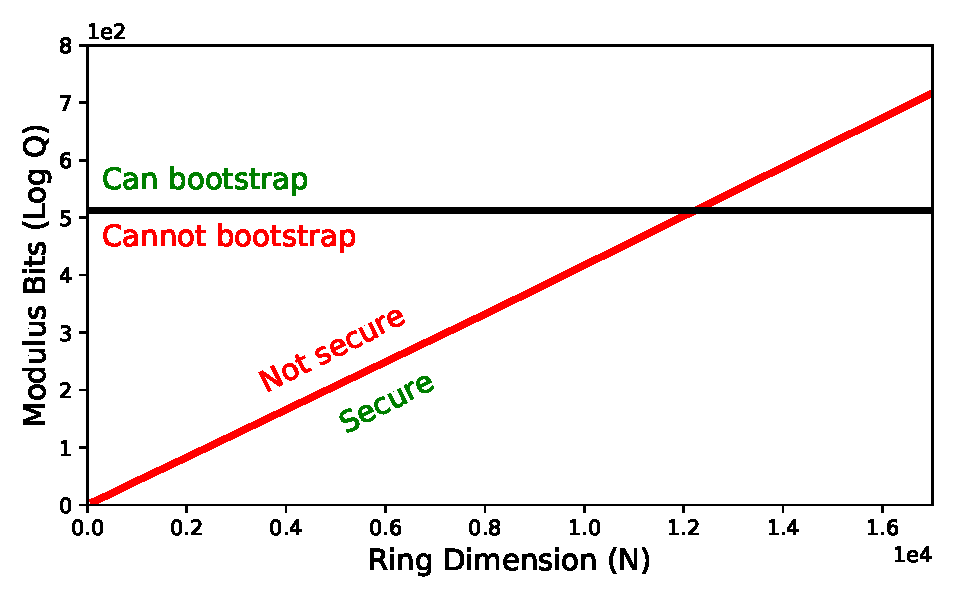
\includegraphics[width=0.75\columnwidth]{plots/security.pdf}
    \caption{Trade-offs between FHE parameters. Parameter values above the
      red line are deemed insecure (i.e., correspond to a security parameter below $80$ bits). The
      parameter values below the black line do not allow for bootstrapping.}
    \label{fig:paramTradeoffs}
    \vspace{-0.03in}
    \end{center}
  \end{figure}
}

\newcommand{\figArch}{
  \begin{figure}[h]
        \begin{center}
     \includegraphics[width=\columnwidth]{figures/ag_arch.pdf}
     \vspace{-0.12in} % this negative vspace... adds space  (which is what I want)
     \caption{Overview of the \name architecture.}
     \vspace{0.025in} % leave bottoms flush
    \label{fig:arch}
  \end{center}
  \end{figure}
}

\newcommand{\figMultDataflow}{
  \begin{figure}[h]
        \begin{center}
     \includegraphics[width=0.99\columnwidth]{figures/ag_mult_dataflow.pdf}
    \caption{Example matrix-vector multiply using FHE.}
    \label{fig:MultDataflow}
    \vspace{-0.1in}
    \end{center}
  \end{figure}
}

\newcommand{\figOpBreakdown}{
    \begin{figure}[h]
    \begin{center}
        \includegraphics[width=0.7\columnwidth]{plots/lolaptwTimeplot.pdf}
        \caption{Functional unit and HBM utilization over time for the LoLa-MNIST PTW benchmark.}
        \label{fig:opBreakdown}
    \end{center}
    \end{figure}
}

\newcommand{\figCompilerOverview}{
  \begin{figure}[h]
        \begin{center}
     \includegraphics[width=\columnwidth]{figures/ag_compiler_overview.pdf}
    \caption{Overview of the \name compiler.}
    \label{fig:compilerOverview}
    %\vspace{-0.06in} %dsm: Shaves off a line, but looks bad
    \end{center}
  \end{figure}
}

\newcommand{\figautfu}{
\setlength{\columnsep}{7pt}
  \begin{figure}[h]
    \begin{center}
      \vspace{-0.8em}
     \includegraphics[width=0.25\columnwidth]{figures/ag_aut_fu.pdf}
    \caption{Automorphism unit.}
    \label{fig:aut_fu}
    \vspace{-0.4em} 
    \end{center}
  \end{figure}
}

\newcommand{\figAutomorphism}{
  \begin{figure}[h]
        \begin{center}
    \includegraphics[width=0.99\columnwidth]{figures/ag_automorphism.pdf}
    \caption{Applying $\sigma_3$ on a ciphertext of four 4-element chunks by using only permutations local to chunks.}
    \label{fig:automorphism}
    \end{center}
  \end{figure}
}

\newcommand{\figTranspose}{
  \begin{figure}[h]
    \centering
    \includegraphics[width=0.5\columnwidth]{figures/ag_transpose.pdf}
    \caption{The transpose unit.}
    \label{fig:transpose}
  \end{figure}
}

\newcommand{\figFourStepNTT}{
  \begin{figure}[h]
    \includegraphics[width=0.99\columnwidth]{figures/ag_four_step_ntt.pdf}
    \caption{Example of a four-step NTT datapath that uses 4-point NTTs to implement 16-point NTTs.}
    \label{fig:fourStepNTT}
    \vspace{1em}
  \end{figure}
}

\newcommand{\figQuadrantSwap}{
  \begin{figure}[h]
    \centering
    \includegraphics[width=0.75\columnwidth]{figures/ag_quadrant_swap.pdf}
    \caption{Transpose unit (right) and its component quadrant-swap unit (left).}
    \label{fig:quadrantSwap}
    \vspace{0.1in}
  \end{figure}
}

\newcommand{\figOverview}{
  \begin{figure}[h]
    \centering
    \vspace{-0.11in}
    \includegraphics[width=.8\columnwidth]{figures/ag_overview.pdf}
    \caption{FHE allows a user to securely offload computation to an untrusted server.}
    %old: \caption{Workflow showing how FHE is used to securely offload computation to an untrusted server.}
    \label{fig:overview}
    \vspace{0.2cm}
  \end{figure}
}

\newcommand{\figFUSweep}{
  \begin{figure}[h]
        \begin{center}
     \includegraphics[width=\columnwidth]{plots/sweepFUs.pdf}
    \caption{Performance of our benchmarks with varying number of functional unit clusters.}
    \label{fig:sweepFUs}
    \vspace{-0.03in}
    \end{center}
  \end{figure}
}

\newcommand{\figBWSweep}{
  \begin{figure}[h]
        \begin{center}
     \includegraphics[width=\columnwidth]{plots/sweepBW.pdf}
    \caption{Performance of our benchmarks across various main memory bandwidths.}
    \label{fig:sweepBW}
    \vspace{-0.03in}
    \end{center}
  \end{figure}
}

\newcommand{\figDataMovement}{
\begin{figure}
  \centering
  \subfloat[]{
    \includegraphics[width=0.4\linewidth]{plots/dataMovement.pdf}
    \label{fig:dataMovement}
  }
  \subfloat[]{
    \includegraphics[width=0.4\linewidth]{plots/power.pdf}
    \label{fig:power}
  }
  \caption{Per-benchmark breakdowns of \textbf{(a)} data movement and \textbf{(b)} average power for \name.}
  %\vspace{0.1in}
\end{figure}
}

\newcommand{\figConfigs}{
    % \setlength{\columnsep}{7pt}
  \begin{figure}[h]
    % \vspace{-0.55in}
    \begin{center}
     \includegraphics[width=0.45\columnwidth]{plots/configs.pdf}
    % \vspace{-0.26in}
    \caption{Performance vs. area across \name configurations.}
    \label{fig:pareto}
    % \vspace{-18pt}
    % \hspace{-0.03in}
    \end{center}
  \end{figure}
}

\newcommand{\figScratchpadSweep}{
  \begin{figure}[h]
        \begin{center}
     \includegraphics[width=\columnwidth]{plots/sweepScratchpad.pdf}
    \caption{Performance of our benchmarks across various scratchpad sizes.}
    \label{fig:sweepScratchpad}
    \vspace{-0.03in}
    \end{center}
  \end{figure}
}

\newcommand{\tblGF}{
  \begin{table}[h]
    \begin{center}
      \begin{footnotesize}
        \begin{tabular}{lrrr}
          \toprule
          Component & Area [mm$^2$] & TDP [W] \\
          \midrule
          NTT FU & 2.27 & 4.80  \\
          Automorphism FU & 0.58 & 0.99  \\
          %Transpose & 0.28 & \tmp{???} & - \\
          Multiply FU & 0.25 & 0.60  \\
          Add FU & 0.03 & 0.05  \\
          Vector RegFile (512\,KB) & 0.56 & 1.67 \\
          \textbf{Compute cluster} & 3.97 & 8.75 \\
          (NTT, Aut, 2$\times$ Mul, 2$\times$ Add, RF) & & \\
          \textbf{Total compute} (16 clusters) &  \textbf{63.52} & \textbf{140} \\
          \midrule
          Scratchpad (16$\times$4\,MB banks) & 48.09 & 20.35 \\
          3$\times$NoC (16$\times$16 512\,B bit-sliced~\cite{passas:tocaid12:crossbar}) & 10.02 & 19.65 \\
          Memory interface (2$\times$HBM2 PHYs) & 29.8 & 0.45 \\
          \textbf{Total memory system} &  \textbf{87.91} & \textbf{40.45} \\
          \midrule
          \textbf{Total \name} &  \textbf{151.43} & \textbf{180.45} \\
          \bottomrule
        \end{tabular}
      \end{footnotesize}
    \end{center}
    \vspace{-0.08in}
    \caption{Area and Thermal Design Power (TDP) of \name, and breakdown by component.}
    \label{tbl:GF12}
    \vspace{-0.1in}
  \end{table}
}


\newcommand{\tblNomenclature}{
   \begin{table}[h]
     \begin{footnotesize}
        \begin{center}
           \begin{tabular}{ll}
              \toprule
              \textbf{Param} & \textbf{Definition} \\
              \midrule
               \multicolumn{2}{c}{FHE Parameters} \\
              \midrule
              $N$ & Number of vector elements / polynomial coefficients \\
              $Q$ & Ciphertext modulus \\
              $t$ & Plaintext modulus \\
              \midrule
               \multicolumn{2}{c}{Architecture Parameters} \\
              \midrule
              $L$ & Number of RNS polynomials per ciphertext polynomial \\
              $q_i$ & The $i$-th RNS modulus ($Q = q_0q_1...q_{L-1}$) \\
              $E$ & Number of vector lanes \\
              $V$ & Vector operation initiation interval ($V = N/E$) \\ % dsm: Chimes? I don't know of a good nomenclature for this...
              \bottomrule
           \end{tabular}
           \label{tbl:nomenclature}
        \end{center}
        \caption{Nomenclature of key parameters in this paper.}
     \end{footnotesize}
   \end{table}
}

\newcommand{\tblModMult}{
  \begin{table}[h]
    \begin{footnotesize}
      \begin{center}
        \begin{tabular}{lrrr}
          \toprule
          Multiplier & Area [$\mu$m$^2$] & Power [mW] & Delay [ps] \\
          \midrule
          Barrett & $5,271$ & $18.4$ & 1,317 \\
          Montgomery & $2,916$ & $9.2$ & 1,040 \\
          NTT-friendly & $2,165$ & $5.36$ & 1,000 \\ % assumes q = 2^11m+1
          \midrule
          \textbf{FHE-friendly (ours)} & $1,817$ & $4.1$ & 1,000 \\
          \bottomrule
        \end{tabular}
        \vspace{0.02in}
        \caption{Area, power, and delay of modular multipliers.}
        \label{tbl:modMult}
      \end{center}
    \end{footnotesize}
    \vspace{-0.18in}
  \end{table}
}

\newcommand{\x}{$\times$}


\newcommand{\tblMicrobenchmark}{
  \begin{table}[t]
      % \vspace{-0pt}
      \begin{center}
      \resizebox{\columnwidth}{!}{%
      \begin{tabular}{l|rrr|rrr|rrr}
        \toprule
        & \multicolumn{3}{c|}{$N = 2^{12}$, $\log Q = 109$} &
        \multicolumn{3}{c|}{$N = 2^{13}$, $\log Q = 218$} &
        \multicolumn{3}{c}{$N = 2^{14}$, $\log Q = 438$} \\
        
        & \textbf{\name} & vs.\ CPU & vs.\ HEAX$_\sigma$ & \textbf{\name} & vs.\ CPU & vs.\ HEAX$_\sigma$ & \textbf{\name} & vs.\ CPU & vs.\ HEAX$_\sigma$\\

        \midrule

        % --- NTT

        % N=2**12, logQ = 109
        NTT
        &\textbf{12.8} % our
        &17,148$\times$ % CPU
        &1,600$\times$ % HEAX

        % N=2**13, logQ = 218
        &\textbf{44.8} % our
        &10,736$\times$ % CPU
        &1,733$\times$ % HEAX

        % N=2**14, logQ = 438
        &\textbf{179.2} % our
        &8,838$\times$ % CPU
        &1,866$\times$ % HEAX
        \\
        % --- Automorph. w/out k-s
        
        % N=2**12, logQ = 109
        Automorphism 
        &\textbf{12.8} % our
        &7,364$\times$ % CPU
        &440$\times$ % HEAX

        % N=2**13, logQ = 218   
        &\textbf{44.8} % our
        &8,250$\times$ % CPU
        &426$\times$ % HEAX

        % N=2**14, logQ = 438
        &\textbf{179.2} % our
        &16,957$\times$ % CPU
        &430$\times$ % HEAX
        \\

        \midrule

        % --- Ctxt-Ctxt Mult.

        % N=2**12, logQ = 109    
        Homomorphic multiply
        &\textbf{60} % our - % 60 MULS * 32 * 1/(32) = 60 cycles
        &48,640$\times$ % CPU
        &172$\times$ % HEAX

        % N=2**13, logQ = 218
        &\textbf{300} % our
        &27,069$\times$ % CPU
        &148$\times$ % HEAX

        % N=2**14, logQ = 438
        &\textbf{2,000} % our
        &14,396$\times$ % CPU
        &190$\times$ % HEAX
        \\

        % --- Automorph. w/ k-s

        % N=2**12, logQ = 109    
        Homomorphic permutation
        &\textbf{40} % our
        &17,488$\times$ % CPU
        &256$\times$ % HEAX

        % N=2**13, logQ = 218
        &\textbf{224} % our
        &10,814$\times$ % CPU
        &198$\times$ % HEAX

        % N=2**14, logQ = 438
        &\textbf{1,680} % our
        &6,421$\times$ % CPU
        &227$\times$ % HEAX
        \\
        
        \bottomrule
      \end{tabular}
      }
      %}
      \end{center}
      %\vspace{-5pt}
      \caption{Performance on microbenchmarks: \name's \textbf{reciprocal throughput, in nanoseconds per ciphertext operation} (lower is better) and speedups over CPU and HEAX$_\sigma$ (HEAX augmented with scalar automorphism units) (higher is better).}
      \label{tbl:microbenchmark}
      %\vspace{-3pt} % dsm: Leaves flush with other pages
  \end{table}
    % dsm: Now explained in text
    %\footnotetext[2]{We assume an SRAM array is used to perform an automorphism via random reads because HEAX does not report how they implement automorphisms.}
    %     \footnotetext[3]{We assume throughput is bottleneck on either the automorphism or keyswitching throughput, whichever is smaller.}
}


\newcommand{\tblBenchmark}{
  \begin{table}[t]
    \begin{footnotesize}
      \begin{center}
      \begin{tabular}{lrrr}
        \toprule
        Execution time (ms) on & CPU & \name & Speedup \\
        
        \midrule
        LoLa-CIFAR Unencryp. Wghts. & $1.2\times10^6$ & \textbf{241} & $5,011$\x \\
        LoLa-MNIST Unencryp. Wghts. & $2,960$ & \textbf{0.17} & $17,412$\x \\
        LoLa-MNIST Encryp. Wghts. & $5,431$ & \textbf{0.36} & $15,086$\x \\
        Logistic Regression & $8,300$ & \textbf{1.15} & $7,217$\x \\
        BGV Bootstrapping & ---\footnotemark[2] & \textbf{1.8} & ---\footnotemark[2] \\  % L=24
        CKKS Bootstrapping & $1,554$ & \textbf{1.3} & $1,195$\x \\    % L=24
        \midrule

        \textbf{gmean speedup} &&& 6,471\x \\
        % CKKS Bootstrapping $L=22$ & $1456$ & \textbf{2.2} & $662$\x \\
        % CKKS Bootstrapping $L=20$ & $1314$ & \textbf{1.9} & $692$\x \\
        \bottomrule
      \end{tabular}
   \end{center}
    \vspace{-8pt}
      \hfill\footnotemark[1]{LoLa's release did not include MNIST with encrypted weights, so we reimplemented it in HELib.}\quad\mbox{} \\
      \hfill\footnotemark[2]{BGV bootstrapping in HELib crashes for this input, and we could not find an alternative implementation or fix HELib. We expect \name's speedup to be at least 3,000$\times$}.\quad\mbox{}
    \end{footnotesize}
    \vspace{4pt}
      \caption{Performance of \name and CPU on full FHE benchmarks: execution times in milliseconds
      and \name's speedup.}      
      \label{tbl:benchmark}
      \vspace{-6pt}
  \end{table}
}

\newcommand{\tblPrimitiveOps}{
  \begin{table}[h]
    \begin{footnotesize}
      \begin{center}
        \caption{Operations in BGV \cite{}, CKKS \cite{}, and GSW \cite{} schemes and their constituent
        \textit{primitive operations}, which \name FUs acelerate. BGV and CKKS use very similar FHE operations
        and differ mainly in encryption/decryption.}
        \begin{tabular}{l|rr}
          \toprule
          & \multicolumn{2}{c}{\textbf{Required primitive operations}} \\
          \textbf{Operation} & \textbf{BGV/CKKS} & \textbf{GSW} \\
          \midrule
          Ciphertext add & add & add \\
          Ciphertext mult & NTT, mult & NTT, mult, add \\
          Key switching/relin & NTT, mult, add & N/A \\
          Mod switching & NTT, reduce, add & NTT, reduce, add \\
          Bootstrapping & automorphism, all ops & automorphism, all ops \\
          \bottomrule
        \end{tabular}
        \label{tbl:primitiveOps}
      \end{center}
    \end{footnotesize}
  \end{table}
}

\newcommand{\cipher}{\textsf{Ciphertext}}
\newcommand{\plain}{\textsf{Plaintext Vector}}
\newcommand{\scalar}{\textsf{Plaintext Scalar}}

\newcommand{\tblDSLOps}{
  \begin{table}[h]
    \begin{footnotesize}
      \begin{center}
        \caption{Supported FHE Operations and Types}
        \begin{tabular}{l|r}
            \textbf{Operation} & \textbf{Type}\\
            \midrule
            \textsf{Mul} & $\cipher \times \cipher \rightarrow \cipher$ \\
            \textsf{MulPlaintext} & $\cipher \times \plain \rightarrow \cipher$ \\
            \textsf{MulScalar} & $\cipher \times \scalar \rightarrow \cipher$ \\
            \textsf{Add} & $\cipher \times \cipher \rightarrow \cipher$ \\
            \textsf{AddPlaintext} & $\cipher \times \plain \rightarrow \cipher$ \\
            \textsf{AddScalar} & $\cipher \times \scalar \rightarrow \cipher$ \\
            \textsf{Rotate} & $\cipher \times \scalar \rightarrow \cipher$ \\
            \textsf{ModDown} & $\cipher \times \scalar \rightarrow \cipher$ \\
        \end{tabular}
      \end{center}
    \end{footnotesize}
  \end{table}
}


\newcommand{\tblSensitivity}{
  \begin{table}[h]
    \begin{footnotesize}
      \begin{center}
        \begin{tabular}{lrrr}
            \toprule
            Benchmark & LT NTT & LT Aut & CSR \\
            \midrule
            LoLa-CIFAR Unencryp. Wghts. & 3.5\x & 12.1\x & ---\footnotemark[1] \\
            LoLa-MNIST Unencryp. Wghts. & 5.0\x & 4.2\x & 1.1\x \\
            LoLa-MNIST Encryp. Wghts. & 5.1\x & 11.9\x & 7.5\x \\
            Logistic Regression & 1.7\x & 2.3\x & 11.7\x \\
            BGV Bootstrapping & 1.6\x & 1.1\x & 5.4\x \\
            CKKS Bootstrapping & 1.1\x & 1.2\x & 2.7\x \\
            \midrule
            \textbf{gmean speedup} & 2.5\x & 5.5\x & 4.2\x \\
            \bottomrule
        \end{tabular}
      \end{center}
      \vspace{-8pt}
      \hfill\footnotemark[1]{CSR is intractable for this benchmark.}\quad\mbox{}
    \end{footnotesize}
    \vspace{4pt}
        \caption{Speedups of \name over alternate configurations: %without our contributions:
          LT NTT/Aut = Low-throughput NTT/Automorphism FUs; CSR = Code Scheduling to minimize Register Usage \cite{goodman:ics1988:code}.}
        \label{tbl:sensitivity}
    \vspace{-2pt}
  \end{table}
}

\newcommand{\C}{\textsf{Scalar}}
\newcommand{\V}{\textsf{Vector}}
\newcommand{\q}{\textsf{Modulus}}

\newcommand{\tblISA}{
  \begin{table}[h]
  \begin{footnotesize}
  \begin{center}
  \caption{\name ISA}
  \begin{tabular}{lr}
  \toprule
  Instruction & Type \\
  \midrule
  \texttt{ADD} & $\V \times \V \times \q \rightarrow \V$ \\
  \texttt{ADD\_SCALAR} & $\V \times \C \times \q \rightarrow \V$ \\
  \texttt{MUL} & $\V \times \V \times \q \rightarrow \V$ \\
  \texttt{MUL\_SCALAR} & $\V \times \C \times \q \rightarrow \V$ \\
  \texttt{NTT} & $\V \times \q \rightarrow \V$ \\
  \texttt{INTT} & $\V \times \q \rightarrow \V$ \\
  \texttt{AUTOMORPHISM} & $\V \times \C \rightarrow \V$ \\
  \end{tabular}
  \label{tbl:isa}
  \end{center}
  \end{footnotesize}
  \end{table}
}


%\usepackage[normalem]{ulem}

% dsm: Place new refs last
\newcommand{\zzzNoOpSortToEnd}{}

%\usepackage{xparse} % makes build fail on mads, ???
\usepackage{siunitx}
\usepackage{verbatim}
\usepackage{graphicx,afterpage}
\usepackage{yfonts}
\usepackage{amsmath}
\usepackage{mathtools}
\usepackage{stmaryrd}
\usepackage{amsfonts}
%\usepackage[mathscr]{euscript}
%\usepackage{commath}
\usepackage{calc}
\usepackage{xspace}
\usepackage{listings}
\usepackage{multirow, booktabs}
%\usepackage{paralist} % FIXME(dsm): compactenum/item incompatible with acmart, but we're still using inparaenum...
%\usepackage[keeplastbox]{flushend}
\usepackage{wrapfig}
\usepackage{enumitem}
%\usepackage{enumerate}
\usepackage{caption}
\usepackage[labelformat=simple]{subcaption}
%\usepackage{subfigure}
\usepackage{dblfloatfix} % to allow two-column floats at the bottom of the page

\usepackage{fancyhdr}

%\usepackage[sort,nocompress]{cite} % autosort groups of citations
% Override IEEEtran, restore default citepunct: https://tex.stackexchange.com/a/72932
% (turns [1], [2], [49] -> [1, 2, 49])
%\renewcommand{\citepunct}{,\penalty\citepunctpenalty\,}

% dsm: Better typesetting
%\usepackage[final]{microtype}

% https://tex.stackexchange.com/questions/240141/
\usepackage[T1]{fontenc} % Avoid garbling symbols and accents

%For fancy tables
\usepackage{array} % decent table formatting
\usepackage{rotating}
%\usepackage[usenames,dvipsnames,svgnames,table]{xcolor}
% \definecolor{ltblue}{HTML}{A6CEE3}
% \definecolor{dkblue}{HTML}{1F78B4}
% \definecolor{dkgreen}{HTML}{33A02C}
% \definecolor{ltgreen}{HTML}{B2DF8A}
% \definecolor{dkorange}{HTML}{FF7F00}
% \definecolor{ltorange}{HTML}{FDBF6F}

% asf: stole this from HATS
\lstdefinestyle{custompython}{
 %aboveskip=0in,
 belowskip=0in,
 %abovecaptionskip=0in,
 belowcaptionskip=-10pt,
 %belowcaptionskip=1\baselineskip,
 breaklines=true,
 captionpos=b,
 language=Python,
 showstringspaces=false,
 numbers=left,
 stepnumber=1,
 % dsm: semibold
 basicstyle={\linespread{0.8}\fontseries{sb}\small\ttfamily},
 %basicstyle={\small\ttfamily},
 keywordstyle=\bfseries,
 %% columns=fullflexible,
 xleftmargin=2em,
 frame=single,
 framexleftmargin=2em,
 commentstyle=\itshape\color{green!40!black},
 morekeywords={to,yield},
}

% from figures.pptx
\definecolor{ltred}{HTML}{FB9A99}
\definecolor{dkred}{HTML}{E41A1C}
\definecolor{dkorange}{HTML}{F07F03}
\definecolor{ltorange}{HTML}{F7C090}
\definecolor{dkgreen}{HTML}{3BA32F}
\definecolor{ltgreen}{HTML}{B2E089}
\definecolor{dkblue}{HTML}{2879B4}
\definecolor{ltblue}{HTML}{A6CEE2}
\definecolor{dkpurple}{HTML}{6A3D9A}
\definecolor{ltpurple}{HTML}{CAB1D7}


% Handle author formatting properly
%\newcommand{\ausep}{\hspace{1.5em}}
\newcommand{\fixAcmartBrainDamage}{Axel Feldmann$^\MIT$$^\ast$, Nikola Samardzic$^\MIT$$^\ast$, Aleksandar Krastev$^\MIT$,\\ Srini Devadas$^\MIT$, Ron Dreslinski$^\UM$, Christopher Peikert$^\UM$, Daniel Sanchez$^\MIT$}
\makeatletter
\def\@typeset@author@bx{\bgroup\hsize=\author@bx@wd
  \def\and{\par}\normalbaselines
  \global\setbox\author@bx=\vtop{\if@ACM@sigchiamode\else\centering\fi
    \@authorfont\fixAcmartBrainDamage\par\@affiliationfont
    \@currentaffiliation}\egroup
  \box\author@bx\hspace{\author@bx@sep}%
  \gdef\@currentauthors{}%
  \gdef\@currentaffiliation{}}
\makeatother

%Use this instead of a hyphen to allow the word itself to be hyphenated
\usepackage{hyphenat}
%\usepackage[hyphens]{url}

% More compact paragraphs
\makeatletter
\renewcommand{\paragraph}[1]{\noindent {\bf #1}}
\renewcommand{\subparagraph}[1]{\noindent {\emph{\textbf{#1}}}}
\makeatother

\newcommand{\topbanner}{\textbf{DRAFT --- \input{auto_header.tex}}}
%\newcommand{\topbanner}{\textsc{Under Submission --- Please Do Not Distribute}}

\begin{comment}
% Headers -- comment these for submission
\makeatletter
\def\ps@plain{
  \def\@oddhead{\hbox{}\normalsize\rightmark \hfil \topbanner \hfil}
  \def\@evenhead{\hbox{}\normalsize\rightmark \hfil \topbanner \hfil}
  \def\@oddfoot{\hbox{}\normalsize\rightmark\hfil \thepage \hfil}
  \def\@evenfoot{\hbox{}\normalsize\rightmark\hfil \thepage \hfil}
}
\makeatother
\end{comment}

% submission/web version
%\pagenumbering{arabic}

\captionsetup[figure]{aboveskip=2pt,belowskip=-12pt}

% If you comment hyperref and then uncomment it, make clean first (or kill .aux files)
\definecolor{lcolor}{RGB}{0, 56, 186} % {0, 35, 102}
%\hypersetup{bookmarks=true,breaklinks=true,letterpaper=true,colorlinks,linkcolor=black,citecolor=black,urlcolor=lcolor}
% \usepackage{hyperref}
% \usepackage[bookmarks=true,breaklinks=true,colorlinks,linkcolor=black,citecolor=blue,urlcolor=black]{hyperref}
% \usepackage[pdfa,bookmarks=true,breaklinks=true,colorlinks,linkcolor=.,citecolor=lcolor,urlcolor=black]{hyperref}


\renewcommand{\figureautorefname}{Fig.}
\renewcommand{\subfigureautorefname}{Fig.}
\renewcommand{\sectionautorefname}{Sec.}
\renewcommand{\subsectionautorefname}{Sec.}
\renewcommand{\paragraphautorefname}{Sec.}
\renewcommand{\equationautorefname}{Eq.}

\renewcommand*{\ttdefault}{txtt}


%dsm: all these are retweaked
% Alter some LaTeX defaults for better treatment of figures:
% See p.105 of "TeX Unbound" for suggested values.
% See pp. 199-200 of Lamport's "LaTeX" book for details.
%   General parameters, for ALL pages:
\renewcommand{\topfraction}{0.9}        % max fraction of floats at top
\renewcommand{\bottomfraction}{0.8}     % max fraction of floats at bottom
%   Parameters for TEXT pages (not float pages):
\setcounter{topnumber}{5}
\setcounter{bottomnumber}{5}
\setcounter{totalnumber}{4}     % 2 may work better
\setcounter{dbltopnumber}{5}    % for 2-column pages
\renewcommand{\dbltopfraction}{0.9}     % fit big float above 2-col. text
\renewcommand{\textfraction}{0.07}      % allow minimal text w. figs
%   Parameters for FLOAT pages (not text pages):
\renewcommand{\floatpagefraction}{0.9}  % require fuller float pages
% N.B.: floatpagefraction MUST be less than topfraction !!
\renewcommand{\dblfloatpagefraction}{0.9}       % require fuller float pages

\usepackage{color}
\definecolor{tableaublue}{rgb}{0.44,0.62,0.81}
\definecolor{tableauorange}{rgb}{0.9,0.55,0.25} % original tableau value: {1.,0.62,0.29}
\definecolor{tableaugreen}{rgb}{0.4,0.75,0.36}
\definecolor{tableaured}{rgb}{0.93,0.4,0.36}
\definecolor{tableaupurple}{rgb}{0.68,0.55,0.79}

\usepackage{pifont}
\usepackage{fourier-orns}
\definecolor{darkred}{rgb}{.65,0,0}
\definecolor{darkgreen}{rgb}{0,.5,0}
\definecolor{darkyellow}{rgb}{0.95,.6,0.1}

% names, abbreviations
\usepackage{textcomp}
\newcommand{\resvec}{residue vector }
\newcommand{\resvecs}{residue vectors }


% Author notes

%\newcommand{\kenote}[1]{\textcolor{blue}{\textbf{(Karim: \emph{#1})}}}
%\newcommand{\nikola}[1]{\textcolor{teal}{\textbf{(Nikola: \emph{#1})}}} 
%\newcommand{\axelf}[1]{\textcolor{orange}{\textbf{(Axel: \emph{#1})}}} 

\renewcommand{\thefootnote}{\fnsymbol{footnote}}

\usepackage{comment}
\usepackage{multicol}

\newcommand{\figFOneArch}{
  \begin{figure}[t]
        \begin{center}
        \includegraphics[width=0.7\linewidth]{f1_figures/ag_arch.pdf}
     \caption{Overview of the F1 architecture.}
    \label{fig:f1arch}
  \end{center}
  \end{figure}
}

\newcommand{\figFOneMultDataflow}{
  \begin{figure}[t]
        \begin{center}
     \includegraphics[width=0.7\columnwidth]{f1_figures/ag_mult_dataflow.pdf}
    \caption{Example matrix-vector multiply using FHE.}
    \label{fig:f1MultDataflow}
    \end{center}
  \end{figure}
}

\newcommand{\figFOneOpBreakdown}{
    \begin{figure}[t]
    \begin{center}
        \includegraphics[width=0.65\columnwidth]{f1_plots/lolaptwTimeplot.pdf}
        \caption{Functional unit and HBM utilization over time for the LoLa-MNIST PTW benchmark.}
        \label{fig:f1opBreakdown}
    \end{center}
    \end{figure}
}

\newcommand{\figFOneCompilerOverview}{
  \begin{figure}[t]
        \begin{center}
     \includegraphics[width=0.65\columnwidth]{f1_figures/ag_compiler_overview.pdf}
    \caption{Overview of the F1 compiler.}
    \label{fig:f1compilerOverview}
    \end{center}
  \end{figure}
}

\newcommand{\figFOneautfu}{
\setlength{\columnsep}{12pt}
  \begin{wrapfigure}{r}{0.3\linewidth}
     \includegraphics[width=0.25\columnwidth]{f1_figures/ag_aut_fu.pdf}
    \caption{Automorphism unit.}
    \label{fig:f1aut_fu}
  \end{wrapfigure}
}

\newcommand{\figFOneAutomorphism}{
  \begin{figure}[t]
        \begin{center}
    \includegraphics[width=0.9\columnwidth]{f1_figures/ag_automorphism.pdf}
    \caption{Applying $\sigma_3$ on an RNS polynomial of four 4-element chunks by using only permutations local to chunks.}
    \label{fig:f1automorphism}
    \end{center}
  \end{figure}
}

\newcommand{\figFOneTranspose}{
  \begin{figure}[t]
    \centering
    \includegraphics[width=0.5\columnwidth]{f1_figures/ag_transpose.pdf}
    \caption{The transpose unit.}
    \label{fig:f1transpose}
  \end{figure}
}

\newcommand{\figFOneFourStepNTT}{
  \begin{figure}[t]
    \begin{center}
    \includegraphics[width=0.8\columnwidth]{f1_figures/ag_four_step_ntt.pdf}
    \caption{Example of a four-step NTT datapath that uses 4-point NTTs to implement 16-point NTTs.}
    \label{fig:f1fourStepNTT}
    \end{center}
  \end{figure}
}

\newcommand{\figFOneQuadrantSwap}{
  \begin{figure}[t]
    \centering
    \includegraphics[width=0.8\columnwidth]{f1_figures/ag_quadrant_swap.pdf}
    \caption{Transpose unit (right) and its component quadrant-swap unit (left).}
    \label{fig:f1quadrantSwap}
  \end{figure}
}

\newcommand{\figFOneOverview}{
  \begin{figure}[h] % dsm: acmart crap bleeds onto the second column, makes it hard for this figure to be on top, so make it [h]
    \centering
    \includegraphics[width=\columnwidth]{f1_figures/ag_overview.pdf}
    \caption{FHE allows a user to securely offload computation to an untrusted server.}
    %old: \caption{Workflow showing how FHE is used to securely offload computation to an untrusted server.}
    \label{fig:f1overview}
  \end{figure}
}

\newcommand{\figFOneFUSweep}{
  \begin{figure}[t]
        \begin{center}
     \includegraphics[width=\columnwidth]{f1_plots_unused/sweepFUs.pdf}
    \caption{Performance of our benchmarks with varying number of functional unit clusters.}
    \label{fig:f1sweepFUs}
    \end{center}
  \end{figure}
}

\newcommand{\figFOneBWSweep}{
  \begin{figure}[t]
        \begin{center}
     \includegraphics[width=\columnwidth]{f1_plots_unused/sweepBW.pdf}
    \caption{Performance of our benchmarks across various main memory bandwidths.}
    \label{fig:f1sweepBW}
    \end{center}
  \end{figure}
}

\newcommand{\figFOneDataMovement}{
\begin{figure}
  \centering
  \captionsetup[subfigure]{labelformat=empty}
  \begin{subfigure}[b]{0.4\columnwidth}
    \includegraphics[width=\linewidth]{f1_plots/dataMovement.pdf}
    \caption{}
    \label{fig:f1dataMovement}
  \end{subfigure}
  \hfill %%
  \begin{subfigure}[b]{0.4\columnwidth}
    \includegraphics[width=\linewidth]{f1_plots/power.pdf}
    \caption{}
    \label{fig:f1power}
  \end{subfigure}
  \begin{center}
    (a) \hspace{0.6\columnwidth} (b)
  \end{center}
  \caption{Per-benchmark breakdowns of (a) data movement and (b) average power for F1.}
\end{figure}
}

\newcommand{\figFOneConfigs}{
  \begin{figure}[t]
    \begin{center}
     \includegraphics[width=0.45\columnwidth]{f1_plots/configs.pdf}
    \caption{Performance vs. area across F1 configurations.}
    \label{fig:f1pareto}
    \end{center}
  \end{figure}
}

\newcommand{\figFOneScratchpadSweep}{
  \begin{figure}[t]
        \begin{center}
     \includegraphics[width=\columnwidth]{f1_plots_unused/sweepScratchpad.pdf}
    \caption{Performance of our benchmarks across various scratchpad sizes.}
    \label{fig:f1sweepScratchpad}
    \end{center}
  \end{figure}
}

\newcommand{\tblFOneGF}{
  \begin{table}[t]
    \begin{center}
      \begin{normalsize}
        \begin{tabular}{lrrr}
          \toprule
          Component & Area [mm$^2$] & TDP [W] \\
          \midrule
          NTT FU & 2.27 & 4.80  \\
          Automorphism FU & 0.58 & 0.99  \\
          %Transpose & 0.28 & \tmp{???} & - \\
          Multiply FU & 0.25 & 0.60  \\
          Add FU & 0.03 & 0.05  \\
          Vector RegFile (512\,KB) & 0.56 & 1.67 \\
          \textbf{Compute cluster} & 3.97 & 8.75 \\
          (NTT, Aut, 2$\times$ Mul, 2$\times$ Add, RF) & & \\
          \textbf{Total compute} (16 clusters) &  \textbf{63.52} & \textbf{140.0} \\
          \midrule
          Scratchpad (16$\times$4\,MB banks) & 48.09 & 20.35 \\
          3$\times$NoC (16$\times$16 512\,B bit-sliced~\cite{passas:tocaid12:crossbar}) & 10.02 & 19.65 \\
          Memory interface (2$\times$HBM2 PHYs) & 29.80 & 0.45 \\
          \textbf{Total memory system} &  \textbf{87.91} & \textbf{40.45} \\
          \midrule
          \textbf{Total F1} &  \textbf{151.4} & \textbf{180.4} \\
          \bottomrule
        \end{tabular}
      \end{normalsize}
    \end{center}
    \caption{Area and Thermal Design Power (TDP) of F1, and breakdown by component.}
    \label{tbl:f1GF12}
  \end{table}
}


\newcommand{\tblFOneNomenclature}{
   \begin{table}[t]
     \begin{normalsize}
        \begin{center}
           \begin{tabular}{ll}
              \toprule
              \textbf{Param} & \textbf{Definition} \\
              \midrule
               \multicolumn{2}{c}{FHE Parameters} \\
              \midrule
              $N$ & Number of vector elements / polynomial coefficients \\
              $Q$ & Ciphertext modulus \\
              $t$ & Plaintext modulus \\
              \midrule
               \multicolumn{2}{c}{Architecture Parameters} \\
              \midrule
              $L$ & Number of RNS polynomials per ciphertext polynomial \\
              $q_i$ & The $i$-th RNS modulus ($Q = q_0q_1...q_{L-1}$) \\
              $E$ & Number of vector lanes \\
              $V$ & Vector operation initiation interval ($V = N/E$) \\ % dsm: Chimes? I don't know of a good nomenclature for this...
              \bottomrule
           \end{tabular}
           \label{tbl:f1nomenclature}
        \end{center}
        \caption{Nomenclature of key parameters in this paper.}
     \end{normalsize}
   \end{table}
}

\newcommand{\tblFOneModMult}{
  \begin{table}[t]
    \begin{normalsize}
      \begin{center}
        \begin{tabular}{lrrr}
          \toprule
          Multiplier & Area [$\mu$m$^2$] & Power [mW] & Delay [ps] \\
          \midrule
          Barrett & $5,271$ & $18.40$ & 1,317 \\
          Montgomery & $2,916$ & $9.29$ & 1,040 \\
          NTT-friendly & $2,165$ & $5.36$ & 1,000 \\ % assumes q = 2^11m+1
          \midrule
          \textbf{FHE-friendly (ours)} & $1,817$ & $4.10$ & 1,000 \\
          \bottomrule
        \end{tabular}
        \caption{Area, power, and delay of modular multipliers.}
        \label{tbl:f1modMult}
      \end{center}
    \end{normalsize}
  \end{table}
}


\newcommand{\tblFOneMicrobenchmark}{
  \begin{table*}[t]
    \begin{scriptsize}
      \begin{center}
%\resizebox{\linewidth}{!}{
      \begin{tabular}{l|rrr|rrr|rrr}
        \toprule
        & \multicolumn{3}{c|}{$N = 2^{12}$, $\log Q = 109$} &
        \multicolumn{3}{c|}{$N = 2^{13}$, $\log Q = 218$} &
        \multicolumn{3}{c}{$N = 2^{14}$, $\log Q = 438$} \\

        & \textbf{F1} & vs.\ CPU & vs.\ HEAX$_\sigma$ & \textbf{F1} & vs.\ CPU & vs.\ HEAX$_\sigma$ & \textbf{F1} & vs.\ CPU & vs.\ HEAX$_\sigma$\\

        \midrule

        % --- NTT

        % N=2**12, logQ = 109
        NTT
        &\textbf{12.8} % our
        &17,148$\times$ % CPU
        &1,600$\times$ % HEAX

        % N=2**13, logQ = 218
        &\textbf{44.8} % our
        &10,736$\times$ % CPU
        &1,733$\times$ % HEAX

        % N=2**14, logQ = 438
        &\textbf{179.2} % our
        &8,838$\times$ % CPU
        &1,866$\times$ % HEAX
        \\
        % --- Automorph. w/out k-s

        % N=2**12, logQ = 109
        Automorphism
        &\textbf{12.8} % our
        &7,364$\times$ % CPU
        &440$\times$ % HEAX

        % N=2**13, logQ = 218
        &\textbf{44.8} % our
        &8,250$\times$ % CPU
        &426$\times$ % HEAX

        % N=2**14, logQ = 438
        &\textbf{179.2} % our
        &16,957$\times$ % CPU
        &430$\times$ % HEAX
        \\

        \midrule

        % --- Ctxt-Ctxt Mult.

        % N=2**12, logQ = 109
        Hom. mult.
        &\textbf{60.0} % our - % 60 MULS * 32 * 1/(32) = 60 cycles
        &48,640$\times$ % CPU
        &172$\times$ % HEAX

        % N=2**13, logQ = 218
        &\textbf{300} % our
        &27,069$\times$ % CPU
        &148$\times$ % HEAX

        % N=2**14, logQ = 438
        &\textbf{2,000} % our
        &14,396$\times$ % CPU
        &190$\times$ % HEAX
        \\

        % --- Automorph. w/ k-s

        % N=2**12, logQ = 109
        Hom. rot.
        &\textbf{40.0} % our
        &17,488$\times$ % CPU
        &256$\times$ % HEAX

        % N=2**13, logQ = 218
        &\textbf{224} % our
        &10,814$\times$ % CPU
        &198$\times$ % HEAX

        % N=2**14, logQ = 438
        &\textbf{1,680} % our
        &6,421$\times$ % CPU
        &227$\times$ % HEAX
        \\

        \bottomrule
      \end{tabular}
      %}
      \end{center}
      \caption{Performance on microbenchmarks: F1's \textbf{reciprocal throughput, in nanoseconds per ciphertext operation} (lower is better) and speedups over CPU and HEAX$_\sigma$ (HEAX augmented with scalar automorphism units) (higher is better).}
      \label{tbl:f1microbenchmark}
    \end{scriptsize}
  \end{table*}
    % dsm: Now explained in text
    %\footnotetext[2]{We assume an SRAM array is used to perform an automorphism via random reads because HEAX does not report how they implement automorphisms.}
    %     \footnotetext[3]{We assume throughput is bottleneck on either the automorphism or keyswitching throughput, whichever is smaller.}
}


\newcommand{\tblFOneBenchmark}{
  \begin{table}[t]
    \begin{normalsize}
      \begin{center}
      \begin{tabular}{lrrr}
        \toprule
        Execution time (ms) on & CPU & F1 & Speedup \\

        \midrule
        LoLa-CIFAR Unencryp. Wghts. & $1.2\times10^6$ & \textbf{241} & $5,011$\x \\
        LoLa-MNIST Unencryp. Wghts. & $2,960$ & \textbf{0.17} & $17,412$\x \\
        LoLa-MNIST Encryp. Wghts. & $5,431$ & \textbf{0.36} & $15,086$\x \\
        Logistic Regression & $8,300$ & \textbf{1.15} & $7,217$\x \\
        DB Lookup & $29,300$ & \textbf{4.36} & $6,722$\x \\
        BGV Bootstrapping & $4,390$ & \textbf{2.40} & $1,830$\x \\  % L=24
        CKKS Bootstrapping & $1,554$ & \textbf{1.30} & $1,195$\x \\    % L=24
        \midrule

        \textbf{gmean speedup} &&& $5,432$\x \\
        % CKKS Bootstrapping $L=22$ & $1456$ & \textbf{2.2} & $662$\x \\
        % CKKS Bootstrapping $L=20$ & $1314$ & \textbf{1.9} & $692$\x \\
        \bottomrule
      \end{tabular}
   \end{center}
      \hfill\footnotemark[1]{LoLa's release did not include MNIST with encrypted weights, so we reimplemented it in HELib.}\quad\mbox{}
    \end{normalsize}
      \caption{Performance of F1 and CPU on full FHE benchmarks: execution times in milliseconds
      and F1's speedup.}      
      \label{tbl:f1benchmark}
  \end{table}
}

\newcommand{\tblFOnePrimitiveOps}{
  \begin{table}[t]
    \begin{normalsize}
      \begin{center}
        \caption{Operations in BGV \cite{}, CKKS \cite{}, and GSW \cite{} schemes and their constituent
        \textit{primitive operations}, which F1 FUs acelerate. BGV and CKKS use very similar FHE operations
        and differ mainly in encryption/decryption.}
        \begin{tabular}{l|rr}
          \toprule
          & \multicolumn{2}{c}{\textbf{Required primitive operations}} \\
          \textbf{Operation} & \textbf{BGV/CKKS} & \textbf{GSW} \\
          \midrule
          Ciphertext add & add & add \\
          Ciphertext mult & NTT, mult & NTT, mult, add \\
          Key switching/relin & NTT, mult, add & N/A \\
          Mod switching & NTT, reduce, add & NTT, reduce, add \\
          Bootstrapping & automorphism, all ops & automorphism, all ops \\
          \bottomrule
        \end{tabular}
        \label{tbl:f1primitiveOps}
      \end{center}
    \end{normalsize}
  \end{table}
}

\newcommand{\cipher}{\textsf{Ciphertext}}
\newcommand{\plain}{\textsf{Plaintext Vector}}
\newcommand{\scalar}{\textsf{Plaintext Scalar}}

\newcommand{\tblFOneDSLOps}{
  \begin{table}[t]
    \begin{normalsize}
      \begin{center}
        \caption{Supported FHE Operations and Types}
        \begin{tabular}{l|r}
            \textbf{Operation} & \textbf{Type}\\
            \midrule
            \textsf{Mul} & $\cipher \times \cipher \rightarrow \cipher$ \\
            \textsf{MulPlaintext} & $\cipher \times \plain \rightarrow \cipher$ \\
            \textsf{MulScalar} & $\cipher \times \scalar \rightarrow \cipher$ \\
            \textsf{Add} & $\cipher \times \cipher \rightarrow \cipher$ \\
            \textsf{AddPlaintext} & $\cipher \times \plain \rightarrow \cipher$ \\
            \textsf{AddScalar} & $\cipher \times \scalar \rightarrow \cipher$ \\
            \textsf{Rotate} & $\cipher \times \scalar \rightarrow \cipher$ \\
            \textsf{ModDown} & $\cipher \times \scalar \rightarrow \cipher$ \\
        \end{tabular}
      \end{center}
    \end{normalsize}
  \end{table}
}


\newcommand{\tblFOneSensitivity}{
  \begin{table}[t]
    \begin{normalsize}
      \begin{center}
        \begin{tabular}{lrrr}
            \toprule
            Benchmark & LT NTT & LT Aut & CSR \\
            \midrule
            LoLa-CIFAR Unencryp. Wghts. & 3.5\x & 12.1\x & ---\footnotemark[1] \\
            LoLa-MNIST Unencryp. Wghts. & 5.0\x & 4.2\x & 1.1\x \\
            LoLa-MNIST Encryp. Wghts. & 5.1\x & 11.9\x & 7.5\x \\
            Logistic Regression & 1.7\x & 2.3\x & 11.7\x \\
            DB Lookup & 2.8\x & 2.2\x & ---\footnotemark[1] \\
            BGV Bootstrapping & 1.5\x & 1.3\x & 5.0\x \\
            CKKS Bootstrapping & 1.1\x & 1.2\x & 2.7\x \\
            \midrule
            \textbf{gmean speedup} & 2.5\x & 3.6\x & 4.2\x \\
            \bottomrule
        \end{tabular}
      \end{center}
      \hfill\footnotemark[1]{CSR is intractable for this benchmark.}\quad\mbox{}
    \end{normalsize}
        \caption{Speedups of F1 over alternate configurations: %without our contributions:
          LT NTT/Aut = Low-throughput NTT/Automorphism FUs; CSR = Code Scheduling to minimize Register Usage~\cite{goodman:ics1988:code}.}
        \label{tbl:f1sensitivity}
  \end{table}
}

\providecommand{\C}{\textsf{Scalar}}
\newcommand{\V}{\textsf{Vector}}
\newcommand{\q}{\textsf{Modulus}}

\newcommand{\tblFOneISA}{
  \begin{table}[t]
  \begin{normalsize}
  \begin{center}
  \caption{F1 ISA}
  \begin{tabular}{lr}
  \toprule
  Instruction & Type \\
  \midrule
  \texttt{ADD} & $\V \times \V \times \q \rightarrow \V$ \\
  \texttt{ADD\_SCALAR} & $\V \times \C \times \q \rightarrow \V$ \\
  \texttt{MUL} & $\V \times \V \times \q \rightarrow \V$ \\
  \texttt{MUL\_SCALAR} & $\V \times \C \times \q \rightarrow \V$ \\
  \texttt{NTT} & $\V \times \q \rightarrow \V$ \\
  \texttt{INTT} & $\V \times \q \rightarrow \V$ \\
  \texttt{AUTOMORPHISM} & $\V \times \C \rightarrow \V$ \\
  \end{tabular}
  \label{tbl:f1isa}
  \end{center}
  \end{normalsize}
  \end{table}
}



%% This bit allows you to either specify only the files which you wish to
%% process, or `all' to process all files which you \include.
%% Krishna Sethuraman (1990).

%\typein [\files]{Enter file names to process, (chap1,chap2 ...), or `all' to
%process all files:}
%\def\all{all}
%\ifx\files\all \typeout{Including all files.} \else \typeout{Including only \files.} \includeonly{\files} \fi

\renewcommand{\name}{CraterLake\xspace}
\newcommand{\Nmax}{N_{\textrm{max}}}
\newcommand{\Lmax}{L_{\textrm{max}}}

\begin{document}

% -*-latex-*-
% 
% For questions, comments, concerns or complaints:
% thesis@mit.edu
% 
%
% $Log: cover.tex,v $
% Revision 1.8  2008/05/13 15:02:15  jdreed
% Degree month is June, not May.  Added note about prevdegrees.
% Arthur Smith's title updated
%
% Revision 1.7  2001/02/08 18:53:16  boojum
% changed some \newpages to \cleardoublepages
%
% Revision 1.6  1999/10/21 14:49:31  boojum
% changed comment referring to documentstyle
%
% Revision 1.5  1999/10/21 14:39:04  boojum
% *** empty log message ***
%
% Revision 1.4  1997/04/18  17:54:10  othomas
% added page numbers on abstract and cover, and made 1 abstract
% page the default rather than 2.  (anne hunter tells me this
% is the new institute standard.)
%
% Revision 1.4  1997/04/18  17:54:10  othomas
% added page numbers on abstract and cover, and made 1 abstract
% page the default rather than 2.  (anne hunter tells me this
% is the new institute standard.)
%
% Revision 1.3  93/05/17  17:06:29  starflt
% Added acknowledgements section (suggested by tompalka)
% 
% Revision 1.2  92/04/22  13:13:13  epeisach
% Fixes for 1991 course 6 requirements
% Phrase "and to grant others the right to do so" has been added to 
% permission clause
% Second copy of abstract is not counted as separate pages so numbering works
% out
% 
% Revision 1.1  92/04/22  13:08:20  epeisach

% NOTE:
% These templates make an effort to conform to the MIT Thesis specifications,
% however the specifications can change.  We recommend that you verify the
% layout of your title page with your thesis advisor and/or the MIT 
% Libraries before printing your final copy.
\title{Enabling Real-time Private DNN Inference Using Fully Homomorphic Encryption}

\author{Nikola Samardzic}
% If you wish to list your previous degrees on the cover page, use the 
% previous degrees command:
%       \prevdegrees{A.A., Harvard University (1985)}
% You can use the \\ command to list multiple previous degrees
%       \prevdegrees{B.S., University of California (1978) \\
%                    S.M., Massachusetts Institute of Technology (1981)}
\prevdegrees{B.S. in Computer Science\linebreak
University of California, Los Angeles, 2020}
\department{Electrical Engineering and Computer Science}

% If the thesis is for two degrees simultaneously, list them both
% separated by \and like this:
% \degree{Doctor of Philosophy \and Master of Science}
\degree{Master of Science in Electrical Engineering and Computer Science}

% As of the 2007-08 academic year, valid degree months are September, 
% February, or June.  The default is June.
\degreemonth{May}
\degreeyear{2022}
\thesisdate{May 13, 2022}

%% By default, the thesis will be copyrighted to MIT.  If you need to copyright
%% the thesis to yourself, just specify the `vi' documentclass option.  If for
%% some reason you want to exactly specify the copyright notice text, you can
%% use the \copyrightnoticetext command.  
%\copyrightnoticetext{\copyright IBM, 1990.  Do not open till Xmas.}

% If there is more than one supervisor, use the \supervisor command
% once for each.
\supervisor{Daniel Sanchez}{Associate Professor of Electrical Engineering and Computer Science}

% This is the department committee chairman, not the thesis committee
% chairman.  You should replace this with your Department's Committee
% Chairman.
\chairman{Leslie A. Kolodziejski}{
Professor of Electrical Engineering and Computer Science\\
Chair, Department Committee on Graduate Students}

% Make the titlepage based on the above information.  If you need
% something special and can't use the standard form, you can specify
% the exact text of the titlepage yourself.  Put it in a titlepage
% environment and leave blank lines where you want vertical space.
% The spaces will be adjusted to fill the entire page.  The dotted
% lines for the signatures are made with the \signature command.
\maketitle

% The abstractpage environment sets up everything on the page except
% the text itself.  The title and other header material are put at the
% top of the page, and the supervisors are listed at the bottom.  A
% new page is begun both before and after.  Of course, an abstract may
% be more than one page itself.  If you need more control over the
% format of the page, you can use the abstract environment, which puts
% the word "Abstract" at the beginning and single spaces its text.

%% You can either \input (*not* \include) your abstract file, or you can put
%% the text of the abstract directly between the \begin{abstractpage} and
%% \end{abstractpage} commands.

% First copy: start a new page, and save the page number.
\cleardoublepage
% Uncomment the next line if you do NOT want a page number on your
% abstract and acknowledgments pages.
% \pagestyle{empty}
\setcounter{savepage}{\thepage}
\begin{abstractpage}

\emph{``This innovation that this industry talks about so much is bullshit. Anybody
can innovate. Don't do this `think different'; don't do this big `innovation'
thing. Screw that. It's meaningless. 99\% of it is: get the work done.''}

--- Linus Torvalds
\vspace{1cm}

Fully Homomorphic Encryption (FHE) allows computing on encrypted data, enabling secure offloading of computation to untrusted servers.
Though it provides ideal security, FHE is expensive when executed in software, 4 to 5 orders of magnitude slower than computing on unencrypted data.
These overheads are a major barrier to FHE's widespread adoption.

We present \name, the first FHE accelerator that is programmable, i.e., capable of executing full FHE programs.
\name builds on an in-depth architectural analysis of the characteristics of FHE computations
that reveals acceleration opportunities. \name is a wide-vector processor with novel functional units deeply specialized to FHE primitives, 
such as modular arithmetic, number-theoretic transforms, and structured permutations.

% axelf: tentative?
Due to the static nature of FHE computations, \name uses an exposed ISA, requiring novel compilation techniques to statically schedule all compute and data movement. We design a compiler that efficiently maps FHE programs onto \name hardware and maximizes reuse of on-chip data, helping to reduce data movement bottlenecks. 
The compiler leverages \name's explicitly managed scratchpad to decouple computation from data movement, a necessary ingredient in achieving high performance given the large size of FHE operands.

% This organization provides so much compute throughput that data movement becomes the key bottleneck.
% Thus, \name is primarily designed to minimize 
% data movement.
% Hardware provides an explicitly-managed memory hierarchy and mechanisms to decouple data movement from execution.
% A novel compiler leverages these mechanisms to maximize reuse and schedule off-chip and on-chip data movement.
 
We evaluate \name using cycle-accurate simulation and RTL synthesis.
\name is the first system to accelerate complete FHE programs,
and outperforms state-of-the-art software implementations by gmean 6,500$\times$ and by up to 17,000$\times$.
These speedups counter most of FHE's overheads and enable new applications, like real-time private deep learning in the cloud.

\end{abstractpage}

% Additional copy: start a new page, and reset the page number.  This way,
% the second copy of the abstract is not counted as separate pages.
% Uncomment the next 6 lines if you need two copies of the abstract
% page.
% \setcounter{page}{\thesavepage}
% \begin{abstractpage}
% % $Log: abstract.tex,v $
% Revision 1.1  93/05/14  14:56:25  starflt
% Initial revision
% 
% Revision 1.1  90/05/04  10:41:01  lwvanels
% Initial revision
% 
%
%% The text of your abstract and nothing else (other than comments) goes here.
%% It will be single-spaced and the rest of the text that is supposed to go on
%% the abstract page will be generated by the abstractpage environment.  This
%% file should be \input (not \include 'd) from cover.tex.



% \end{abstractpage}

\cleardoublepage

\section*{Acknowledgments}

Thank you to all the people that created the environment in which success is
easy. Your work matters and changes lives.

This work was conducted in collaboration with Axel Feldmann, Aleksandar
Krastev, Nicholas Genise, Prof. Srini Devadas, Karim Eldefrawy, Nathan Manohar,
Prof. Ron Dreslinski, Prof. Chris Peikert, and my research advisor Prof. Daniel
Sanchez. Much of this thesis is adapted from joinly written papers. This work
would not have been possible without all of their contributions.


%%%%%%%%%%%%%%%%%%%%%%%%%%%%%%%%%%%%%%%%%%%%%%%%%%%%%%%%%%%%%%%%%%%%%%
% -*-latex-*-

% Some departments (e.g. 5) require an additional signature page.  See
% signature.tex for more information and uncomment the following line if
% applicable.
% \include{signature}
\pagestyle{plain}
  % -*- Mode:TeX -*-
%% This file simply contains the commands that actually generate the table of
%% contents and lists of figures and tables.  You can omit any or all of
%% these files by simply taking out the appropriate command.  For more
%% information on these files, see appendix C.3.3 of the LaTeX manual.
\tableofcontents
\newpage
%\listoffigures
%\newpage
%\listoftables


\section{Introduction}\label{sec:intro}

A large and increasing fraction of the world's compute runs on the cloud,
which is vulnerable to data breaches.
Conventional techniques to mitigate attacks offer limited 
security, as cloud servers must decrypt data in order to process it.

\emph{Fully homomorphic encryption (FHE)} is a special type of encryption scheme
that enables \emph{computing on encrypted data directly}, without decrypting it.
FHE allows a client to offload a computation
to an untrusted server \emph{without} revealing any data (\autoref{fig:workflow}).
This enables the client to harness the compute power of the cloud while maintaining cryptographic privacy.
Though FHE has some limitations (e.g., data-dependent branching is not possible), 
it is general enough to support many compelling use cases,
such as privacy-preserving machine learning, secure genome analysis, private set intersection,
private information retrieval, and many more~\cite{kim2020semi,gilad:icml16:cryptonets,han:aaai19:logistic,han:iacr18:efficient,juvekar2018gazelle,DBLP:conf/ccs/ChenLR17,DBLP:conf/tcc/GentryH19}. 
%\nnote{add citations and more examples}

% axelf: purging unfortunately/fortunately from the whole paper
Despite its ideal privacy, FHE is rarely used today because it incurs prohibitive overheads:
in CPUs, FHE computations are 10,000$\times$ to 100,000$\times$
slower than equivalent unencrypted computations, even when using highly optimized FHE libraries.
% dsm: I don't think this adds much here, other than distance to get to the actual point
%Some of these overhead costs are due
%to the size of FHE ciphertexts while
%others are due to the additional complexity
%of representing arbitrary functions in a form suitable for
% computing using FHE.

Fortunately, state-of-the-art FHE schemes are well-suited to hardware acceleration.
First, they are regular and structured:
FHE programs operate on very long vectors, and all operations are known ahead of time.
Second, FHE requires several non-SIMD operations,
such as \emph{number-theoretic transforms} (NTTs),
that are inefficient on CPUs and GPUs.
But these operations can be accelerated by specialized functional units,
avoiding these inefficiencies.
As a result, prior work has proposed FPGA and ASIC-based
accelerators~\cite{riazi:asplos20:heax,cousins:hpec12:sipher-fpga,cousins:tetc17:fpga-he,turan:tc20:heaws,cousins:hpec14:fpga-he, roy:hpca19:fpga-he,feldmann:micro21:f1}.
While most prior accelerators achieve limited speedups, a recent design,
F1~\cite{feldmann:micro21:f1}, achieves speedups of
%2,000-15,000$\times$ 
% dsm: Let's avoid the 15000x speedup, we don't have anything that large but we're using a different baseline, diff configs, etc.
about 5,000$\times$
on FHE programs.

% dsm: Unfortunately here is important. We were just describing potential, we want to signpost that we're entering negative territory.
Unfortunately, prior accelerators are efficient only on a limited subset of simple FHE
computations---those of \emph{shallow multiplicative depth}.
% FIXME(dsm): I think this may be from edits, but right now several terms are left undefined: DEPTH and MULTIPLICATIVE DEPTH. I think this is because the text below does not talk about multiplications.
For example, prior FHE accelerators can run neural network inference efficiently only for networks with few layers (3-6),
but they cannot accelerate state-of-the-art deep neural networks (DNNs) with tens to hundreds of layers.

This limitation stems from the characteristics of FHE schemes:
each ciphertext has some associated noise, which grows with each homomorphic operation, and especially with multiplications.
If noise becomes too large, it garbles the message, making decryption impossible. 
%To support computations with higher multiplicative depth, the size of ciphertexts must increase to counteract the additional noise growth, resulting in each FHE operation being more computationally expensive.
Larger ciphertexts tolerate more noise before becoming undecryptable. 
However, operations on larger ciphertexts are also more expensive.
To enable computations of unbounded depth, ciphertexts can be ``refreshed'' using a procedure called \emph{bootstrapping}
that reduces noise. But bootstrapping is expensive, 
% dsm: multiplicative depth is NOT YET DEFINED
%and itself consumes multiplicative depth, 
so ciphertexts must be very large (10s of MBs) for bootstrapping to be
efficient.

Prior FHE accelerators do not efficiently handle unbounded-depth computations because
they natively support vectors of a limited size and they use algorithms that scale poorly
to the large ciphertexts in high-depth programs.
As a result, they can only run small FHE computations, and they do not support sufficient depth
to run the full bootstrapping procedure.

\figWorkflow

In this paper we tackle this challenge through \name, the first FHE accelerator
to support \emph{FHE computations of unbounded depth}.
To achieve this, we contribute new algorithms, specialized functional units,
hardware architecture, and compiler techniques that overcome the key challenge
of deep FHE computations---its extreme data movement demands.

\paragraph{Deep FHE is limited by data movement:}
FHE schemes encode information over very long vectors of wide elements.
Concretely, supporting unbounded-depth computations requires vectors of
64K elements with 1,600 bits per element.
This takes 25\,MB per ciphertext, 12$\times$ larger than what prior FHE accelerators target.
% nikola; 25MB = 2 * 1600 bits * 64*1024 elements * (1/8) bytes / bit * 1/2^20 bytes / MB

% (alex): I changed the comparisson from to 32 MB to 23 MB ciphertexts;
%         Being charittable, this is L = 1500/32 = 46 for F1 and KSH is 23*46 = 1058MB
% nikola: 2MB ciphertext in F1 => 1MB per ciphertext polynomial => 512 bits per coeff at N=16K
% => L = 16 (32-bit moduli) => KSH = 2*L^2*N * 32 bits / elem = 32 MB
% nikola: 26MB ciphertext in F1 => 13MB per ciphertext polynomial + assume N=64K
% => log Q = 1,664 => L = 52 => KSH = 2*L^2*N * 32 bits / elem * (1/8) B/bit * 1/2^30 GB/B
% = 1.32 GB
% At the same log Q = 1,664, CL needs L = 1664/28 = 60: KSH = 2*2*L*N = 
% = 2*2 * 60 (L) * 64*1024 (N) * 28 bits / elem * (1/8) B/bit * 1/2^20 MB/B = 52.5 MB
% (note that L is actually 1668/26.7, but we divide by 28 to be consistent with the F1
% methodology, where we multiply by 32)
Moreover, prior work has employed FHE algorithms that require even larger amounts of auxiliary data.
For example, multiplying 2\,MB ciphertexts in F1~\cite{feldmann:micro21:f1} requires 32\,MB of auxiliary data,
and scaling their algorithm to 26\,MB ciphertexts would require over
1.3\,GB 
of auxiliary data---far too large to fit on-chip.
To tackle this challenge, our \emph{key insight} is to adopt an FHE
algorithm called \emph{boosted keyswitching} (\autoref{sec:keyswitching}) that eliminates most of the
auxiliary data,
% (alex): KSH it's 2 ciphertexts without PRG
reducing this overhead from 1.3\,GB to 52.5\,MB.
%We further reduce this overhead to 23\,MB by introducing a new functional unit that
%generates half of this auxiliary data on the fly, rather than fetching it from memory.
Boosted keyswitching also reduces computation costs.
However, this new algorithm is a poor match for prior accelerators:
it is dominated by simple operations where these designs have limited efficiency,
and makes poor use of the specialized functional units that prior designs leverage.

Beyond being inefficient, prior accelerators suffer from a hard-to-scale vector multicore architecture:
to support the needed non-SIMD operations with reasonable cost,
they implement multiple independent cores with narrower vector datapaths~\cite{feldmann:micro21:f1}.
However, this causes excessive inter-core communication,
and the high-bandwidth interconnect
needed grows superlinearly with the number of cores.


\paragraph{Deep FHE demands new hardware techniques:}
To tackle these challenges, we introduce the \emph{\name} architecture (\autoref{sec:overview}, \autoref{sec:architecture}),
the first FHE accelerator that achieves high performance on unbounded FHE programs.
\name is a wide-vector uniprocessor with specialized functional units.
The design is statically scheduled to leverage the regularity of FHE computations.
We contribute several new techniques that make this possible, including:
\begin{compactitem}
\item A new extremely wide (2,048 lanes) vector uniprocessor architecture that
    spreads each vector operation across the chip, departing from prior vector multicore architectures.
The uniprocessor approach reduces the number of concurrent operations, which minimizes footprint,
  reducing off-chip traffic, and simplifies the compiler.
\item An efficient implementation of the above architecture, which is challenging for non-SIMD FHE operations, NTTs and automorphisms,
  by decomposing these operations in a novel way that allows the use of a \emph{fixed transpose network} among physically distributed groups of lanes.
  This reduces on-chip data movement and interconnect cost over prior approaches.
\item A new functional unit that encapsulates the bulk of operations in boosted keyswitching, improving efficiency and enabling high utilization across ciphertexts of all sizes.
\item A new functional unit that generates half of the required auxiliary data on the fly (reducing overheads from 52\,MB to 26\,MB), saving on-chip storage and memory bandwidth.
\item A vector chaining technique that builds long FU pipelines to enable many concurrent operations with few register ports.
\end{compactitem}
To program \name, we develop a novel compiler (\autoref{sec:compiler}) that produces efficient code from high-level FHE programs.
The compiler schedules operations to maximize reuse, decouples data movement from computation,
and adapts the state-of-the-art bootstrapping algorithm to achieve high
utilization~\cite{bossuat:crypto21:efficient}.


We evaluate \name through a combination of simulation and RTL synthesis (to find its area and power).
We use a broad range of FHE benchmarks, including programs with high multiplicative depth
that require bootstrapping.
\name outperforms a scaled-up and improved version of the state-of-the-art FHE accelerator, F1, by gmean 
11.2$\times$ on these deep computations,
and is 4,600$\times$ faster than a 32-core CPU.
These speedups enable new use cases for FHE.
For example, deep neural networks like ResNet
% which takes tens of \emph{minutes} per inference on CPUs,
% nikola: again, it really takes tens of minutes, but that's cuz of hours algo improvements
% dsm: Let's not confuse the reader, we can mention that this used to be hours in the eval but saying hours to ms is comparing apples to oranges
take 23 minutes per inference on the CPU,
whereas \name achieves 250 \emph{milliseconds} per inference,
enabling real-time private deep learning.
% 23 minutes = 1.37694e+12 ns / (10^9*60) = 22.9 min
% 265 ms = 2.64245e+08 / (10^6) = 264 ms


\chapter{Background}\label{sec:background}
% \nikola{need to introduce the NTT somewhere in this section; probably after data representation}
% \nikola{need to define an automorphism in this section; probably when defining homomorphic rotation}
% \nnote{referring to CKKS as an FHE scheme even though it's only for approximate arithmetic... people sometimes complain about this}


% CKKS\footnote{named after the authors}~\cite{ckks}
% is an FHE scheme that supports encrypted computations on vectors of real numbers.
% CKKS ciphertexts are a pair of degree-$N$ polynomials with coefficients
% being large integers modulo some $Q$. Common parameter
% regimes include $N$ from $1K$ to $64K$ and $\log_2(Q)$
% from $1K$ to $2K$.
% Choosing $N$ and $Q$ for proper performance
% and security depends on the program you want to run, and is an active area of
% research~\cite{DBLP:conf/crypto/May21}.
% For this reason, we focus exclusively on optimizing
% the performance of CKKS, although our accelerator can also be
% used for other FHE schemes.


State-of-the-art % dsm: Unless this is TFHE jab, why? nikola: The point is that in theory there may exist yet-undiscovered FHE schemes that work really well but dont operate on encrypted vectors :P
FHE schemes implement operations on~\emph{encrypted vectors}.
The FHE ciphertexts in these schemes support several \emph{homomorphic operations}:
element-wise addition, element-wise multiplication, and cyclic rotations of vector elements.
Each homomorphic operation produces a ciphertext that, when decrypted,
produces the same result as if the operation had been performed on the unencrypted inputs.

Importantly, homomorphic operations have a different implementation from their unencrypted counterparts---for example,
a homomorphic multiplication is not implemented using element-wise multiplication
of the input ciphertexts, but a more complex
sequence of operations. Therefore, it is useful to differentiate between FHE's \emph{interface},
i.e., its supported plaintext datatypes and operations,
and its \emph{implementation},
i.e., the structure of ciphertexts and the implementation of homomorphic operations.

There are several FHE schemes, which mainly differ in their plaintext datatypes and the operations they support.
For example, BGV~\cite{brakerski:toct14:leveled} encodes vectors of integers modulo a constant,
whereas CKKS~\cite{cheon:ictaci17:homomorphic} encodes vectors of fixed-point numbers.
Despite the differences between these schemes, % all state-of-the-art FHE schemes
%use a similar format for ciphertexts, as they rely on the hardness of the same problem
%(LWE or ring-LWE~\cite{lyubashevsky:tact10:ideal}) to attain security.
%have similarities since they all rely on the hardness of learning with errors (LWE) or its ring variant (ring-LWE)~\cite{lyubashevsky:tact10:ideal} to attain security.
the commonalities in their underlying implementation~\cite{lyubashevsky:tact10:ideal}
make it possible for the same hardware to
accelerate many schemes
efficiently---\name supports CKKS, BGV, and GSW~\cite{gentry:crypto13:homomorphic}.
For concreteness, the rest of this section will focus only on CKKS as it
is the scheme best suited for machine learning tasks and has been the focus of
recent work in FHE algorithms~\cite{han:iacr18:efficient,lee:2021:privacy,gilad:icml16:cryptonets,podschwadt:2020:classification,dathathri:pldi19:chet,dathathri:pldi20:eva}.

\subsection{FHE Interface}

%State-of-the-art % dsm: Whatever, once was enough
FHE schemes implement operations on vectors of values.
In CKKS, each vector element is a \emph{fixed-point} complex number with a configurable number of bits.
(Programs that do not use complex arithmetic can zero out the imaginary part.)
% with a set number of quotient and mantissa bits. % nikola: confusing % dsm: why?
% nikola: this is confusing because it is the definition of fixed point.
% so why put it there? As a reminder? That's alright, but I would add "i.e." or
% something
% dsm: No, it is important because architects are used to thinking about FIXED FORMATS, like fp32, bfloat16, etc. We must say that the number of bits is configurable.

Since values are encrypted, FHE does not permit data-dependent branching or indirection.
Thus, all operations and dependencies are known ahead of time, and FHE programs can
be represented using \emph{static dataflow graphs}.

% nikola: regarding Daniel's note on arbitrarily vs relatively. It _is_ true
% that we can make computation arbitrarily precise (just add bits of precision!).
Homomorphic operations in CKKS include element-wise addition, element-wise multiplication,
and cyclic rotations.
While these operations are \emph{approximate} in CKKS, inducing a small and
controllable amount of error, this error can be made arbitrarily small at the
cost of reduced performance. % \nnote{this is only true for a priori bounded-depth computation, but i think it's fine to not mention this}
% dsm: Someone changed arbitrarily to relatively. Unless this error absolutely cannot be reduced beyond a non-zero threshold, please don't fudge it. I don't care that it's expensive and it's not done in practice. Digital logic is also expensive vs analog, and wasn't considered practical for a long time, yet here we are. I'm trying to distance this from the minefield thsat is approximate computing.
This error is acceptable in practice as machine learning applications
are insensitive to it.

FHE exposes a vector programming model with a restricted set of operations; in particular,
FHE does not provide access to individual vector elements.
This makes it challenging to implement some operations
that are trivial in plaintext:
For example,
implementing a convolutional layer of a neural network requires the careful
replication of filter weights.
The lack of non-linear functions introduces other difficulties.
For example, the ReLU activation function must be approximated
using a high-degree polynomial~\cite{lee:2021:precise}.
%
As a result, faithfully replicating deep neural networks in FHE,
as done by a recent ResNet implementation~\cite{lee:2021:privacy}, comes at a high compute cost.
However, recent work has proposed neural network structures that are optimized
for FHE and achieve higher performance while maintaining similar accuracy~\cite{brutzkus:icml19:low}.
We evaluate \name on both styles of neural networks.

Finally, not all data needs to be encrypted:
additions and multiplications are much cheaper in FHE if one of the operands is unencrypted.
This allows algorithms to trade privacy for performance.
For example, running a neural network using unencrypted weights is faster; it
still ensures the privacy of inputs and results, but does not
protect weights~\cite{brutzkus:icml19:low}.

\subsection{FHE Implementation}

% \nnote{some FHE schemes are actually quite different, so i changed the wording here a bit. also, GSW is kind of different from BGV and CKKS}
We now describe how CKKS represents and operates on encrypted data (i.e., ciphertexts);
other schemes (e.g., BGV) have a similar structure.

\paragraph{Encryption:} A ciphertext holds an encrypted vector of plaintext values.
To create a ciphertext, the vector of plaintext values is first encoded, or \emph{packed},
in a polynomial; this polynomial is then \emph{encrypted}.
CKKS packs a plaintext vector of $ n = N/2$ complex fixed-point numbers
into a degree-$(N-1)$ polynomial:
% dsm: Sinbce this modulus doesn;t show up anywhere else, and it's unclear how you would pick t to support fixed-point numbers, I'm killing it.
%with integer coefficients modulo a plaintext
%modulus $t$:
\begin{equation*}
    (c_0, c_1, ..., c_n) \xmapsto{pack} \mathfrak{m} = k_0 + k_1x + ... + k_{N-1}x^{N-1} %\in R_q
\end{equation*}
% NOTE(dsm): Do not call m a plaintext.
$\mathfrak{m}$ is then encrypted into a ciphertext. Each ciphertext consists of
% nikola: better to call these ct_0, ct_1 instead of p_0, p_1 cuz then the homomorphic add example makes more sense (i.e., ct. polys are named after the ciphertext + an index)
$\mathfrak{ct}_0, \mathfrak{ct}_1$---two \emph{ciphertext polynomials}
with coefficients modulo a \emph{ciphertext modulus} $Q$.
Specifically, we encrypt $\mathfrak{m}$
under a \emph{secret key} $\mathfrak{s}$
by sampling a uniformly random $\mathfrak{a}$
and a small \emph{error} $\mathfrak{e}$ ($\mathfrak{s}$, $\mathfrak{a}$, and $\mathfrak{e}$ are also polynomials):
% nikola: change the above remark to a footnote instead of writing \in R_Q because s and e are *just* polynomials, and a is actually in R_Q. This distinction doesnt matter for ISCA, so I just say they are all polynomials, which is correct. But saying they are all in R_Q would actually be incorrect, so I forgoe it
\begin{equation*}
    \mathfrak{m} \xmapsto{encrypt} \mathfrak{ct} = (\mathfrak{ct}_0, \mathfrak{ct}_1) = (\mathfrak{a}, \mathfrak{a}\cdot\mathfrak{s}+\mathfrak{e}+\mathfrak{m})
\end{equation*}
% dsm: Comment out if low on space... but we do use partially packed later on.
The above process produces a \emph{fully-packed} ciphertext, i.e., one
that encodes as many plaintext values as possible. It is possible
(though almost always less efficient) to pack~fewer~values,
producing a partially packed or unpacked (one-element) ciphertext.

% dsm: We need to be careful with how this is described, it seems like this is horribly approximate and the interface is already talking about the error. Positionaing this as approximate computing would be a strategic mistake.
%The noise term is necessary for the message $m$ to be cryptographically secure.
%Also, note how the message's low-order bits are corrupted by the error.
%This often does not interfere with the final computation
%since computations done with CKKS are convergent and CKKS's
%encoding mechanism accounts for the error-message interaction,
%i.e.\ the significant bits are encoded well above the error.
%The latter is because the noise growth in each FHE computation is predictable.


\paragraph{Homomorphic operations} are implemented through several modular-arithmetic operations on ciphertext polynomials, i.e., vectors of coefficients. Specifically:
\begin{compactitem}
\item \emph{Homomorphic addition} of two ciphertexts simply requires modular addition of their ciphertext polynomials:
    $\mathfrak{ct}_{\textrm{add}} = \mathfrak{a} + \mathfrak{b} = (\mathfrak{a}_0+\mathfrak{b}_0, \mathfrak{a}_1+\mathfrak{b}_1)$.
\item \emph{Homomorphic multiplication} is implemented using polynomial multiplications and additions;
  multiplying two polynomials requires convolving their coefficients.
% nikola: there was a convolving elements thing here... this is confusing. I would just say it this way.
% dsm: Nikola, the whole point is to make it crystal clear thea POLYNOMAIL MULTIPLICATION != MULTIPLICATION. Otherwise the NTT will ome as a complete surprise.
\item \emph{Homomorphic rotation} rotates the vector encrypted~in~a~ciphertext.
  Implementing it requires performing an \emph{automorphism} on the ciphertext polynomials,
  % nikola: there is no benefit to us in explaining what automorphisms are (this is different from F1, where this was critical as it was one of our contributions).
  % we can just leave it like above (i.e., automorphism is some fairy dust you sprinkle and you get homomorphic rotates).
  % Actually explainin what an automorphism is causes unnecessary confusion. It's hard enough to remember that homomorphic rotations cyclically rotate the vector.
  % dsm: I disagree. This paper needs to be self-contained! We ARE using F1's approach to implement automorphisms, but if you don't explain them even superficially, epople will jump to barrel shifters, etc.
  a structured permutation where, for automorphism $k$, each input index $i$ is mapped to output index $ik \bmod N$.
  There are $N$ possible automorphisms; each automorphism induces a simpler, cyclic rotation in the plaintext.

\end{compactitem}

On top of this, homomorphic multiplications and rotations also require a procedure called \emph{keyswitching},
which is needed so that the final ciphertext
stays encrypted by the same secret key as the input.
Keyswitching is expensive, and, in practice, \emph{takes over 90\% of all operations}.
Keyswitching is central to \name, so we discuss it in detail in \autoref{sec:keyswitching}.

%Homomorphic addition of ciphertexts
%$\mathfrak{a} = (\mathfrak{a}_0, \mathfrak{a}_1)$ and
%$\mathfrak{b} = (\mathfrak{b}_0, \mathfrak{b}_1)$
%is done simply by adding their corresponding polynomials:
%$ct_{\textrm{add}} = \mathfrak{a} + \mathfrak{b} = (\mathfrak{a}_0+\mathfrak{b}_0, \mathfrak{a}_1+\mathfrak{b}_1)$.
%Homomorphic rotations, on a ciphertext encrypting plaintext $(c_0, c_1, ..., c_n)$,
%are done by ciphertext automorphisms. These are signed permutations
%on the ciphertext coefficients which allow a user to homomorphically
%rotate the plaintext values. There are $n$ such automorphisms,
%but they are generated by one automorphism representing cyclic
%plaintext shift. One can combine these rotations with plaintext
%multiplications (with a 0-1 plaintext vector) to perform any
%permutation homomorphically.

%Some other operations are also straightforward: specifically,
%ciphertext-plaintext additions / multiplications,
%plaintext rotations.
%However, ciphertext-ciphertext multiplications and ciphertext rotations are computationally
%expensive; they require 10-100 polynomial operations. This is because these operations
%require \emph{keyswitching}, a crucial homomorphic suboperation that is responsible
%for over $90$\% of polynomial operations on all of our benchmarks. We discuss
%keyswitching in detail in \autoref{sec:keyswitching}.

%The implementation of homomorphic multiplication is shown in
%\autoref{listing:homomorphicMult}.

\subsection{Algorithmic insights and optimizations}\label{sec:algoInsights}
\label{sec:fhe_optimizations}

F1 leverages two optimizations developed in prior work:

\paragraph{Fast polynomial multiplication via NTTs:}
Multiplying two polynomials requires convolving their coefficients, an
expensive (naively $O(N^2)$) operation.
Just like convolutions can be made faster with the Fast Fourier Transform,
polynomial multiplication can be made faster with the Number-Theoretic Transform (NTT)~\cite{moenck1976practical},  % victor asked for a  ``reassuring read-more-about-NTT citation''
a variant of the discrete Fourier transform for modular arithmetic.
The NTT takes an $N$\hyp{}coefficient polynomial as input and returns an $N$\hyp{}element vector representing the input in the
\textit{NTT domain}. Polynomial multiplication can be performed as element-wise multiplication in the NTT domain. Specifically,
\begin{equation*}
    NTT(\mathfrak{a}\mathfrak{b}) = NTT(\mathfrak{a}) \odot NTT(\mathfrak{b}),
\end{equation*}
where $\odot$ denotes component-wise multiplication.
(For this relation to hold with $N$\hyp{}point NTTs, a \emph{negacyclic} NTT~\cite{lyubashevsky:tact10:ideal} must be used (\autoref{sec:fourStepNTT}).)

Because an NTT requires only $O(N \log N)$ modular operations,
multiplication can be performed in $O(N \log N)$ operations by using two forward NTTs,
element-wise multiplication, and an inverse NTT.
And in fact, optimized FHE implementations often store polynomials in the NTT domain
rather than in their coefficient form \emph{across operations}, further reducing the number of NTTs.
This is possible because the NTT is a linear transformation, so additions and automorphisms can also be performed in the NTT domain:
\vspace{-0.05in} % FIXME(dsm): Terrible break
\begin{align*}
    NTT(\sigma_k(\mathfrak{a})) &= \sigma_k(NTT(\mathfrak{a})) \\
    NTT(\mathfrak{a} + \mathfrak{b}) &= NTT(\mathfrak{a}) + NTT(\mathfrak{b})
\end{align*}
\vspace{-0.2in}

\paragraph{Avoiding wide arithmetic via Residue Number System (RNS) representation:}
FHE requires wide ciphertext coefficients (e.g., 512 bits), but wide arithmetic is expensive:
the cost of a modular multiplier (which takes most of the compute)
grows quadratically with bit width in our range of interest.
Moreover, \mbox{we need to efficiently} % HACK(dsm): Fix acmart brain damage and bad break
support a broad range of widths (e.g., 64 to 512 bits in 32-bit increments),
both because programs need different widths, and because modulus switching progressively reduces coefficient widths.

RNS representation \cite{garner1959residue}  % victor asked for a ``reassuring read-more-about-RNS citation''
enables representing a single polynomial with wide coefficients as multiple polynomials with narrower coefficients,
called \emph{residue polynomials}.
To achieve this, the modulus~$Q$  is chosen to be the product of $L$
smaller distinct primes, $Q = q_1q_2\cdots\ q_L$.
Then, a polynomial in $R_Q$ can be represented as $L$ polynomials in
$R_{q_1}, \ldots, R_{q_L}$,
where the coefficients in the $i$-th polynomial are simply the wide coefficients modulo $q_i$.
%
For example, with $W = 32$-bit words, a ciphertext polynomial with $512$-bit modulus~$Q$ is represented as
$L = \log Q/W = 16$ polynomials with $32$-bit coefficients.

All FHE operations can be carried out under RNS representation, and have either better or equivalent bit-complexity than
  operating on one wide-coefficient polynomial.
  %For example, using an RNS representation of a polynomial of length $N$, addition
%requires $2NL$ $32$-bit additions module the $q_i$s, and a homomorphic multiplication requires $L^2$ NTTs, $2L^2$ 32-bit
%coefficient multiplications, and $2L^2$ 32-bit additions.

\subsection{Architectural analysis of FHE}
\label{sec:fhe_analysis}

We now analyze a key FHE kernel in depth to understand how we can (and cannot) accelerate it.
Specifically, we consider the the standard keyswitching operation,
which is expensive and takes the majority of work in all of F1's benchmarks.
CraterLake implements \emph{boosted} keyswitching, a variant of keyswitching more amenable
to acceleration (\autoref{sec:keyswitching}); however, F1 does not target boosted keyswitching.
Nonetheless, many of the conclusions from this section carry over to the boosted keyswitching setting.

\autoref{listing:keyswitch} shows an implementation of standard keyswitching.
Standard keyswitching takes three inputs: a polynomial \texttt{x}, and two
\emph{keyswitch hint matrices} \texttt{ksh0} and \texttt{ksh1}. \texttt{x} is
stored in RNS form as $L$ residue polynomials (\texttt{RVec}). Each residue
polynomial \texttt{x[i]} is a vector of $N$ 32-bit integers modulo $q_i$.
Inputs and outputs are in the NTT domain; only the \texttt{y[i]} polynomials
(line 3) are in coefficient form.


% dsm: RPoly is confusing, because most of these are NOT the coefficients of a polynomial.
\begin{figure}
\begin{center}
  \begin{lstlisting}[caption={Standard keyswitch implementation. \texttt{RVec} is an $N$-element vector of 32-bit values, storing a single RNS polynomial in either the coefficient or the NTT domain.
    }, mathescape=true, style=custompython, label=listing:keyswitch]
  def keySwitch(x: RVec[L],
        ksh0: RVec[L][L], ksh1: RVec[L][L]):
    y = [INTT(x[i],$q_i$) for i in range(L)]
    u0: RVec[L] = [0, ...]
    u1: RVec[L] = [0, ...]
    for i in range(L):
      for j in range(L):
        xqj = (i == j) ? x[i] : NTT(y[i], $q_j$)
        u0[j] += xqj * ksh0[i,j] mod $q_j$
        u1[j] += xqj * ksh1[i,j] mod $q_j$
    return (u0, u1)
  \end{lstlisting}
\end{center}
\end{figure}

%Each automorphism, in addition to ciphertext multiplication, requires a different pair of key-switch hint matrices.

\paragraph{Computation vs.\ data movement:}
A single key-switch requires $L^2$ NTTs, $2L^2$ multiplications, and $2L^2$
additions of $N$-element \mbox{vectors}. In RNS form, the rest of a homomorphic
multiplication (excluding key-switching) is $4L$ multiplications and $3L$
additions (\autoref{sec:fhe_operation}), so key-switching is dominant.

However, the main cost at high values of $L$ and $N$ is data movement. For
example, at $L = 16$, $N = 16K$, each RNS polynomial (\texttt{RVec}) is 64\,KB;
each ciphertext polynomial is 1\,MB; each ciphertext is 2\,MB; and the
key-switch hints dominate, taking up 32\,MB. With F1's compute throughput,
fetching the inputs of each key-switching from off-chip memory would demand
about 10\,TB/s of memory bandwidth. Thus, it is crucial to reuse these values
as much as possible.

Fortunately, keyswitch hints can be reused: all homomorphic multiplications
use the same keyswitch hint matrices, and each automorphism has its own pair
of matrices. But values are so large that few of them fit on-chip.

Finally, note that there is no effective way to decompose or tile this
operation to reduce storage needs while achieving good reuse: tiling the
keyswitch hint matrices on either dimension produces many long-lived
intermediate values; and tiling across \texttt{RVec} elements is even worse
because in NTTs every input element affects every output element.

\paragraph{Performance requirements:}
We conclude that, to accommodate these large operands, an FHE accelerator
requires a memory system that \emph{(1)} decouples data movement from
computation, as demand misses during frequent key-switches would tank
performance; and \emph{(2)} implements a large amount of on-chip storage (over
32\,MB in our example) to allow reuse across entire homomorphic operations
(e.g., reusing the same key-switch hints across many homomorphic
multiplications).

Moreover, the FHE accelerator must be designed to use the memory system well.
First, scheduling data movement and computation is crucial: data must be
fetched far ahead of its use to provide decoupling, and operations must be
ordered carefully to maximize reuse. Second, since values are large, excessive
parallelism can increase footprint and hinder reuse. Thus, the system should
use relatively few high-throughput functional units rather than many
low-throughput ones.

\paragraph{Functionality requirements:}
Programmable FHE accelerators must support a wide range of parameters, both $N$
(polynomial/vector sizes) and $L$ (number of RNS polynomials, i.e., number of
32-bit prime factors of $Q$). While $N$ is generally fixed for a single
program, $L$ changes as modulus switching sheds off polynomials.

Moreover, FHE accelerators must avoid overspecializing in order to support algorithmic diversity.
For instance, we have described \emph{an} implementation of keyswitching, but
there are others~\cite{kim:jmir18:helr,gentry:crypto2012:homomorphic}
with different tradeoffs.

F1 accelerates \emph{primitive operations on large vectors}:
modular arithmetic, NTTs, and automorphisms. It exploits wide vector processing
to achieve very high throughput, even though this makes NTTs and automorphisms
costlier. F1 avoids building functional units for coarser primitives, like
key-switching, which would hinder algorithmic diversity.

\subsection{Challenges of Deep FHE Computation}\label{sec:deepChallenges}

FHE ciphertexts include some \emph{noise} or \emph{error} %(the $\mathfrak{e}$
term above) to ensure cryptographic privacy~\cite{lyubashevsky:tact10:ideal}.
Noise compounds during homomorphic operations, which adds overheads. Noise
increases primarily during ciphertext multiplications; each ciphertext can
tolerate only a fixed amount of noise before decryption becomes impossible.
Therefore, we say that the \emph{multiplicative depth} a ciphertext can
tolerate is the ciphertext's \emph{multiplicative budget}.

Supporting a high multiplicative budget requires using ciphertexts with wide
coefficients and a large ciphertext modulus $Q$. For example, ciphertexts with
512-bit coefficients have a multiplicative budget of about 16. After each
multiplication, the ciphertext is \emph{rescaled} to use a smaller modulus
(e.g., dropping 32 bits).
This trims the noise and makes computation more efficient over time, as
narrower coefficients are cheaper to operate on. Ciphertexts run out of
multiplicative depth when their coefficients become too narrow to support
further operations (e.g., 32 bits). In CKKS, the specific number of bits to
drop per operation is not fixed, but depends on the precision that the
application requires.

A high multiplicative depth computation can be supported by simply using
ciphertexts with sufficiently high multiplicative budgets, but this adds major
overheads. First, it requires using very wide coefficients, which take more
storage per plaintext element and make computations more complex. Moreover,
wide coefficients induce a second hurdle: they force the use of larger vectors.
This is because, for security, $N/\log Q$ must be above a certain threshold.
For instance, a multiplicative budget of 16 requires $Q$ of about 512 bits and
$N$=16K (i.e., 2\,MB per ciphertext), and a multiplicative budget of 32
requires $Q$ of about 1,024 bits and $N$=32K (i.e., 8\,MB per ciphertext).
Though larger vectors can pack more plaintext elements, this quickly results in
vectors so large that they cannot fit on-chip. Overall, ciphertext size grows
quadratically with multiplicative budget, and compute cost cubically (inducing
linear and quadratic overheads per plaintext element, respectively).


\figBootstrapping

\paragraph{Bootstrapping:} FHE schemes limit the overheads of deep computation
through a procedure called bootstrapping that refreshes the multiplicative
budget of a ciphertext. Bootstrapping enables computations of arbitrary depth
by separating them into regions of limited depth. But
bootstrapping~is~an~expensive and deep computation, so it should happen
infrequently.

\autoref{fig:bootstrapping} illustrates a typical evolution of a ciphertext's
multiplicative budget during execution of a program: computation proceeds until
the ciphertext runs out of budget, then bootstrapping is applied to refresh the
ciphertext. For example, in our LSTM benchmark, computation starts with a
multiplicative budget of 57 and bootstrapping consumes the highest 35 levels
(in red in \autoref{fig:bootstrapping}), leaving 22 levels for application
computation (in blue in \autoref{fig:bootstrapping}).


\paragraph{Ciphertext sizes needed for deep FHE:}
We now show that \name supports the ciphertext sizes required for deep FHE, and
why prior work falls short. \autoref{fig:bootstrappingFrequency} reports the
cost per homomorphic operation (in scalar multiplies per homomorphic multiply,
$y$-axis) of two deep programs, as a function of the maximum ciphertext size
used ($x$-axis). This determines bootstrapping frequency: using larger
ciphertexts requires less frequent bootstrapping.
\autoref{fig:bootstrappingFrequency} also breaks down cost by~that used for
application computation (blue) and bootstrapping (red).

The left plot is for a serial chain of multiplies, the worst case for
bootstrapping cost, as the amount of computation between bootstrappings is
minimal. Consequently, bootstrapping cost dominates. By contrast, the right
plot is for a very wide graph with 100 multiplies per depth, which converge to
a single output after each level. This allows boostrapping to be amortized
across many operations, a best-case scenario.

Crucially, the optimal choice of maximum ciphertext size (shown with a black
dot) is in a narrow range for both extremes, between 20\,MB (right) and 26\,MB
(left). This is because \emph{both} application computation and bootstrapping
become more expensive with ciphertext size, so regardless of which dominates,
once bootstrapping is infrequent enough, moving to larger ciphertexts only
hurts performance.

Thus, 20--26\,MB max ciphertexts are the sweet spot for most deep programs,
which fall between these extremes. In practice, bootstrapping placement is
NP-hard~\cite{benhamouda2017optimization}, because real FHE programs are not as
regular. But all our benchmarks show a similar tradeoff curve to these
synthetic programs.

\figBootstrappingFrequency

\emph{Prior FHE accelerators cannot efficiently support ciphertexts this large}.
For example, F1~\cite{feldmann:micro21:f1} \emph{becomes inefficient past
2\,MB}. Prior accelerators~\cite{riazi:asplos20:heax} are limited to even
smaller values. This is insufficient to run even bootstrapping itself.
(Although F1 supports \emph{unpacked} bootstrapping of ciphertexts that encode
only a single element, this is $>$1,000$\times$ slower per element and thus
impractical for full applications, as \autoref{sec:results} shows.)

As we will see, scaling to large ciphertexts is not merely a matter of scaling
up hardware; it requires new algorithms and a new hardware organization to
support these algorithms and to cope with the huge footprint of ciphertexts.

\subsection{CraterLake vs. F1}

Though F1 is programmable and can accelerate full computations, it targets
shallow computations. Specifically, F1 is tailored to a keyswitching algorithm
that does not scale to high multiplicative budgets $L$
(\autoref{sec:keyswitching}). As a result, F1 is inefficient when using a more
scalable keyswitching algorithm: It has an inappropriate mix of functional
units, and even with the right mix, it would be dominated by simple operations
that would require over 100 register file ports for the FUs to be fully
utilized.
Moreover, F1's organization incurs excessive communication and is hard to scale
to larger systems.

As a result, \name introduces a fundamentally different design, needed for deep
computations: it adopts a new, simpler hardware organization and data tiling
approach that reduces communication and scales to the large ciphertexts
required, and it is tailored to use an efficient keyswitching algorithm, which
requires new functional units and optimizations.

\subsection{Prior FHE Accelerators and Their Limitations}\label{sec:drawbacks}


Prior work has proposed several FHE accelerators for
FPGAs~\cite{cousins:hpec14:fpga-he,cousins:tetc17:fpga-he,doroz:tc15:accelerating-fhe,roy:hpca19:fpga-he,migliore:tecs17:he-karatsuba,riazi:asplos20:heax,turan:tc20:heaws,mert:tvlsi20:bfv-accel}.
These systems have three important limitations. First, they work by
accelerating some primitives but defer others to a general-purpose host
processor, and rely on the host processor to sequence operations. This causes
excessive data movement that limits speedups. Second, these accelerators build
functional units for \emph{fixed parameters} $N$ and $L$ (or $\log Q$ for those
not using RNS). Third, many of these systems build overspecialized primitives
that limit algorithmic diversity.

Most of these systems achieve limited speedups, about 10$\times$ over software
baselines. HEAX~\cite{riazi:asplos20:heax} achieves larger speedups
(200$\times$ vs.\ a single core). But it does so by overspecializing: it uses
relatively low-throughput functional units for primitive operations, so to
achieve high performance, it builds a fixed-function pipeline for
keyswitching.

\chapter{F1}
\section{F1 Architecture}\label{sec:f1_arch}

\autoref{fig:f1arch} shows an overview of F1, which we derive from the insights
in \autoref{sec:fhe_analysis}.

\paragraph{Vector processing with specialized functional units:}
F1 features wide-vector execution with functional units (FUs) tailored to
primitive FHE operations. Specifically, F1 implements vector FUs for modular
addition, modular multiplication, NTTs (forward and inverse in the same unit),
and automorphisms. Because we leverage RNS representation, these FUs use a
fixed, small arithmetic word size (32 bits in our implementation), avoiding
wide arithmetic.

FUs process vectors of configurable \emph{length} $N$ using a fixed number of
\emph{vector lanes} $E$. Our implementation uses $E=$128 lanes and supports
power-of-two lengths $N$ from 1,024 to 16,384. This covers the common range of
FHE polynomial sizes, so an RNS polynomial maps to a single vector. Larger
polynomials (e.g., of 32K elements) can use multiple vectors.

All FUs are \emph{fully pipelined}, so they achieve the same throughput of
$E=128$ elements/cycle. FUs consume their inputs in contiguous chunks of $E$
elements in consecutive cycles. This is easy for element-wise operations, but
hard for NTTs and automorphisms. \autoref{sec:f1_fus} details our novel FU
implementations, including the first vector implementation of automorphisms.
F1's evaluation shows that these FUs achieve much higher performance than those
of prior work. This is important because, as we saw in
\autoref{sec:fhe_analysis}, \emph{having fewer high-throughput FUs reduces
parallelism and thus memory footprint}.

\paragraph{Compute clusters:}
Functional units are grouped in \emph{compute clusters}, as
\autoref{fig:f1arch} shows. Each cluster features several FUs (1 NTT, 1
automorphism, 2 multipliers, and 2 adders in our implementation) and a banked
register file that can (cheaply) supply enough operands each cycle to keep all
FUs busy. The chip has multiple clusters (16 in our implementation).

\figFOneArch

\paragraph{Memory system:}
F1 features an explicitly managed memory hierarchy. As \autoref{fig:f1arch}
shows, F1 features a large, heavily banked scratchpad (64\,MB across {16} banks
in our implementation). The scratchpad interfaces with both high-bandwidth
off-chip memory (HBM2 in our implementation) and with compute clusters through
an on-chip network.

F1 uses decoupled data orchestration~\cite{pellauer:asplos19:buffets} to hide
main memory latency. Scratchpad banks work autonomously, fetching data from
main memory far ahead of its use. Since memory has relatively low bandwidth,
off-chip data is always staged in scratchpads, and compute clusters do not
access main memory directly.

The on-chip network connecting scratchpad banks and compute clusters provides
very high bandwidth, which is necessary because register files are small and
achieve limited reuse. We implement a single-stage bit-sliced crossbar
network~\cite{passas:tocaid12:crossbar} that provides full bisection bandwidth.
Banks and the network have wide ports (512 bytes), so that a single scratchpad
bank can send a vector to a compute unit at the rate it is consumed (and
receive it at the rate it is produced). This avoids long staging of vectors at
the register files.

\paragraph{Static scheduling:}
Because FHE programs are completely regular, F1 adopts a \emph{static, exposed
microarchitecture}: all components have fixed latencies, which are exposed to
the compiler. The compiler is responsible for scheduling operations and data
transfers in the appropriate cycles to prevent structural or data hazards. This
is in the style of VLIW processors~\cite{fisher:isca83:very}.

Static scheduling simplifies logic throughout the chip. For example, FUs need
no stalling logic; register files and scratchpad banks need no dynamic
arbitration to handle conflicts; and the on-chip network uses simple switches
that change their configuration independently over time, without the buffers
and arbiters of packet-switched networks.

Because memory accesses do have a variable latency, we assume the worst-case
latency, and buffer data that arrives earlier (note that, because we access
large chunks of data, e.g., 64\,KB, this worst-case latency is not far from the
average).

\paragraph{Distributed control:}
Though static scheduling is the hallmark of VLIW, F1's implementation is quite
different: rather than having a single stream of instructions with many
operations each, in F1 each component has an \emph{independent instruction
stream}. This is possible because F1 does not have any control flow: though FHE
programs may have loops, we unroll them to avoid all branches, and compile
programs into linear sequences of instructions.

This approach may appear costly. But vectors are very long, so each instruction
encodes a lot of work and this overhead is minimal. Moreover, this enables a
compact instruction format, which encodes a single operation followed by the
number of cycles to wait until running the next instruction. This encoding
avoids the low utilization of VLIW instructions, which leave many operation
slots empty. Each FU, register file, network switch, scratchpad bank, and
memory controller has its own instruction stream, which a control~unit~fetches
in small blocks and distributes to components. Overall, instruction fetches
consume less than 0.1\% of memory traffic.

\paragraph{Register file (RF) design:}
Each cluster in F1 requires 10 read ports and 6 write ports to keep all FUs
busy. To enable this cheaply, we use an 8-banked \emph{element-partitioned}
register file design~\cite{asanovic:ucb98:vector} that leverages long vectors:
each vector is striped across banks, and each FU cycles through all banks over
time, using a single bank each cycle. By staggering the start of each vector
operation, FUs access different banks each cycle. This avoids multiporting,
requires a simple RF-FU interconnect, and performs within 5\% of an ideal
infinite-ported RF.

\section{Scheduling Data and Computation}\label{sec:f1_scheduler}

We now describe F1's software stack, focusing on the new static scheduling
algorithms needed to use hardware well.

\figFOneCompilerOverview

\autoref{fig:f1compilerOverview} shows an overview of the F1 compiler. The
compiler takes as input an FHE program written in a high-level domain specific
language (\autoref{sec:programming}). The compiler is structured in three
stages. First, the \emph{homomorphic operation compiler} orders high-level
operations to maximize reuse and translates the program into a
\emph{computation dataflow graph}, where operations are computation
instructions but there are no loads or stores. Second, the \emph{off-chip data
movement scheduler} schedules transfers between main memory and the scratchpad
to achieve decoupling and maximize reuse. This phase uses a simplified view of
hardware, considering it as a scratchpad directly attached to functional units.
The result is a dataflow graph that includes loads and stores from off-chip
memory. Third, the \emph{cycle-level scheduler} refines this dataflow graph. It
uses a cycle-accurate hardware model to divide instructions across compute
clusters and schedule on-chip data transfers. This phase determine the exact
cycles of all operations, and produces the instruction streams for all
components.

This multi-pass scheduling primarily minimizes off-chip data movement, the
critical bottleneck. Only in the last phase do we consider on-chip placement
and data movement.

\paragraph{Comparison with prior work:}
We initially tried static sched\-uling algorithms from prior
work~\cite{blelloch:acm1999:provably,marchal:jpdc2019:limiting,goodman:ics1988:code,ozer:micro1998:unified,barany:odes2011:register},
which primarily target VLIW architectures. However, we found these approaches
ill-suited to F1 for multiple reasons. First, VLIW designs have less-flexible
decoupling mechanisms and minimizing data movement is secondary to maximizing
compute operations per cycle. Second, prior algorithms often focus on loops,
where the key concern is to find a compact repeating schedule, e.g., through
software pipelining~\cite{lam1989software}. By contrast, F1 has no flow control
and we can schedule each operation independently. Third, though prior work has
proposed register-pressure-aware instruction scheduling algorithms, they
targeted small register files and basic blocks, whereas we must manage a large
scratchpad over a much longer horizon. Thus, the algorithms we tried either
worked poorly~\cite{ozer:micro1998:unified, goodman:ics1988:code,
marchal:jpdc2019:limiting} or could not scale to the sizes
required~\cite{barany:odes2011:register, xu:sigplan2007:tetris,
touati:ijpp2005:register, berson:pact1993:ursa}.

For example, when considering an algorithm such as Code Scheduling to Minimize
Register Usage (CSR)~\cite{goodman:ics1988:code}, we find that the schedules it
produces suffer from a large blowup of live intermediate values. This large
footprint causes scratchpad thrashing and results in poor performance.
Furthermore, CSR is also quite computationally expensive, requiring long
scheduling times for our larger benchmarks. We evaluate our approach against
CSR in \autoref{sec:sensitivity}.

We also attempted to frame scheduling as a register allocation problem.
Effectively, the key challenge in all of our schedules is \emph{data movement},
not computation. Finding a register allocation which minimizes spilling could
provide a good basis for an effective schedule. However, our scratchpad stores
at least 1024 residue vectors (1024 at maximum $N = 16K$, more for smaller
values of $N$), and many of our benchmarks involve hundreds of thousands of
instructions, meaning that register allocation algorithms simply could not
scale to our required sizes~\cite{barany:odes2011:register,
xu:sigplan2007:tetris, touati:ijpp2005:register, berson:pact1993:ursa}.

\subsection{Translating the Program to a Dataflow Graph}
\label{sec:programming}

We implement a high-level domain-specific language (DSL) for writing F1
programs. To illustrate this DSL and provide a running example,
\autoref{listing:mv} shows the code for matrix-vector multiplication. This
follows HELib's algorithm~\cite{halevi:crypto14:algorithms}, which
\autoref{fig:f1MultDataflow} shows. This toy $4 \times 16K$ matrix-vector
multiply uses input ciphertexts with $N=16K$. Because accessing individual
vector elements is not possible, the code uses homomorphic rotations to produce
each output element.

\figFOneMultDataflow

\begin{figure}
\begin{center}
  \begin{lstlisting}[caption={$(4 \times 16K)$ matrix-vector multiply in F1's DSL.}, mathescape=true, style=custompython, label=listing:mv]
p = Program(N = 16384)
M_rows = [ p.Input(L = 16) for i in range(4) ]
output = [ None for i in range(4) ]
V = p.Input(L = 16)

def innerSum(X):
  for i in range(log2(p.N)):
    X = Add(X, Rotate(X, 1 << i))
  return X

for i in range(4):
  prod = Mul(M_rows[i], V)
  output[i] = innerSum(prod)
  \end{lstlisting}
\end{center}
\vspace{0.15cm}
\end{figure}

As \autoref{listing:mv} shows, programs in this DSL are at the level of the
simple FHE interface presented in \autoref{sec:fhe_mapping}. There is only one
aspect of the FHE implementation in the DSL: programs encode the desired noise
budget ($L=16$ in our example), as the compiler does not automate noise
management.

\subsection{Compiling Homomorphic Operations}

The first compiler phase works at the level of the homomorphic operations
provided by the DSL. It clusters operations to improve reuse, and translates
them down to instructions.

\paragraph{Ordering} homomorphic operations seeks to maximize the reuse of
keyswitch hints, which is crucial to reduce data movement
(\autoref{sec:fhe_analysis}). For instance, the program in \autoref{listing:mv}
uses 15 different sets of keyswitch hints: one for the multiplies (line
12), and a different one for \emph{each} of the rotations (line 8). If this
program was run sequentially as written, it would cycle through all 15
keyswitch hints (which total 480\,MB, exceeding on-chip storage) four times,
achieving no reuse. Clearly, it is better to reorder the computation to perform
all four multiplies, and then all four \texttt{Rotate(X, 1)}, and so on. This
reuses each keyswitch hint four times.

To achieve this, this pass first clusters \emph{independent} homomorphic
operations that reuse the same hint, then orders all clusters through simple
list-scheduling. This generates schedules with good keyswitch hint reuse.

\paragraph{Translation:} Each homomorphic operation is then compiled into
instructions, using the implementation of each operation in the target FHE
scheme (BGV, CKKS, or GSW). Each homomorphic operation may translate to
thousands of instructions. These instructions are also ordered to minimize the
amount of intermediates. The end result is an instruction-level dataflow graph
where every instruction is tagged with a priority that reflects its global
order.

The compiler exploits algorithmic choice. Specifically, there are multiple
implementations of keyswitching (\autoref{sec:fhe_analysis},
\autoref{sec:boostedKeyswitching}), and the right choice depends on $L$, the
amount of keyswitch reuse, and load on FUs. The compiler leverages knowledge of
operation order to estimate these and choose the right variant.

\subsection{Scheduling Data Transfers}
\label{sec:datatransfers}

The second phase of F1's compiler consumes an instruction-level dataflow graph
and produces an approximate schedule that includes data transfers decoupled
from computation, minimizes off-chip data transfers, and achieves good
parallelism. This requires solving an interdependent problem: when to bring a
value into the scratchpad and which one to replace depends on the computation
schedule; and to prevent stalls, the computation schedule depends on which
values are in the scratchpad. To solve this problem, this scheduler uses a
simplified model of the machine: it does not consider on-chip data movement,
and simply treats all functional units as being directly connected to the
scratchpad.

The scheduler is greedy, scheduling one instruction at a time. It considers
instructions ready if their inputs are available in the scratchpad, and follows
instruction priority among ready ones. To schedule loads, we assign each load a
priority

\begin{equation*}
p(\text{load}) = \max \{ p(u) | u \in users(\text{load})\},
\end{equation*}

then greedily issue loads as bandwidth becomes available. When issuing an
instruction, we must ensure that there is space to store its result. We can
often replace a dead value. When no such value exists, we evict the value with
the furthest expected time to reuse. We estimate time to reuse as the maximum
priority among unissued users of the value. This approximates Belady's optimal
replacement policy~\cite{belady1966study}. Evictions of dirty data add stores
to the dataflow graph. When evicting a value, we add spill (either dirty or
clean) and fill instructions to our dataflow graph.

\subsection{Cycle-Level Scheduling}

Finally, the cycle-level scheduler takes in the data movement schedule produced
by the previous phase, and schedules all operations for all components
considering all resource constraints and data dependences. This phase
distributes computation across clusters and manages their register files and
all on-chip transfers. Importantly, this scheduler is fully constrained by its
input schedule's off-chip data movement. It does not add loads or stores in
this stage, but it does move loads to their earliest possible issue cycle to
avoid stalls on missing operands. All resource hazards are resolved by
stalling. In practice, we find that this separation of scheduling into data
movement and instruction scheduling produces good schedules in reasonable
compilation times.

This stage works by iterating through all instructions in the order produced by
the previous compiler phase (\autoref{sec:datatransfers}) and determining the
minimum cycle at which all required on-chip resources are available. We
consider the availability of off-chip bandwidth, scratchpad space, register
file space, functional units, and ports.

During this final compiler pass, we finally account for store bandwidth,
scheduling stores (which result from spills) as needed. In practice, we find
that this does not hurt our performance much, as stores are infrequent across
most of our benchmarks due to our global schedule and replacement policy
design. After the final schedule is generated, we validate it by simulating it
forward to ensure that no clobbers or resource usage violations occur.

It is important to note that because our schedules are fully static, our
scheduler also doubles as a performance measurement tool. As illustrated in
\autoref{fig:f1compilerOverview}, the compiler takes in an architecture
description file detailing a particular configuration of F1. This flexibility
allows us to conduct design space explorations very quickly
(\autoref{sec:scalability}).

\section{Functional Units}
\label{sec:f1_fus}

In this section, we describe F1's novel functional units. These include the
first vectorized automorphism unit (\autoref{sec:automorphism}), the first
fully-pipelined flexible NTT unit (\autoref{sec:fourStepNTT}), and a new
simplified modular multiplier adapted to FHE (\autoref{sec:modMult}).

\subsection{Automorphism Unit}\label{sec:automorphism}

\figFOneAutomorphism

Because F1 uses $E$ vector lanes, each residue polynomial is stored and
processed as $G$ groups, or \emph{chunks}, of $E$ elements each ($N=G\cdot E$).
An automorphism $\sigma_k$ maps the element at index $i$ to index $k\cdot i \textrm{
mod } N$; there are $N$ automorphisms total, two for each odd $k < N$
(\autoref{sec:fhe_operation}). The key challenge in designing an automorphism
unit is that these permutations are hard to vectorize: we would like this unit
to consume and produce $E=128$ elements/cycle, but the vectors are much longer,
with $N$ up to $16K$;w, and elements are permuted across different chunks.
Moreover, we must support variable $N$ \emph{and} all automorphisms.

Standard solutions fail: a $16K\times16K$ crossbar is much too large; a
scalar approach, like reading elements in sequence from an SRAM, is too slow
(taking $N$ cycles); and using banks of SRAM to increase throughput runs into
frequent bank conflicts: each automorphism ``spreads''~elements with a
different stride, so regardless of the banking scheme, some automorphisms will
map many consecutive elements to the~same~bank.

We contribute a new insight that makes vectorizing automorphisms simple: if we
interpret a residue polynomial as a $G \times E$ matrix, an automorphism can
always be decomposed into two independent \emph{column} and \emph{row
permutations}. If we transpose this matrix, both column and row permutations
can be applied \emph{in chunks of $E$ elements}. \autoref{fig:f1automorphism}
shows an example of how automorphism $\sigma_3$ is applied to a residue
polynomial with $N=16$ and $E=4$ elements/cycle. Note how the permute column
and row operations are local to each $4$-element chunk. Other $\sigma_k$ induce
different permutations, but with the same row/column structure.

\figFOneautfu

F1's automorphism unit, shown in \autoref{fig:f1aut_fu}, uses this insight to be
both vectorized (consuming $E=128$ elements/cycle) and fully pipelined. Given a
residue polynomial of $N=G\cdot E$ elements, the automorphism unit first
applies the column permutation to each $E$-element input. Then, it feeds this
to a \emph{transpose unit} that reads in the whole residue polynomial
interpreting it as a $G\times E$ matrix, and produces its transpose $E\times
G$. The transpose unit outputs $E$ elements per cycle (outputting multiple rows
per cycle when $G < E$). Row permutations are applied to each $E$-element
chunk, and the reverse transpose is applied.

Further, we decompose both the row and column permutations into a pipeline of
sub-permutations that are \textit{fixed in hardware}, with each sub-permutation
either applied or bypassed based on simple control logic; this avoids using
crossbars for the $E$-element permute row and column operations.

\figFOneQuadrantSwap

\paragraph{Transpose unit:}
F1's \textit{quadrant-swap transpose} unit transposes an $E \times E$ (e.g.,
$128\times 128$) matrix by recursively decomposing it into quadrants and
exploiting the identity

\begin{equation*}
  \left[ \begin{array}{c|c}
      \texttt{A} & \texttt{B}\\
      \hline
      \texttt{C} & \texttt{D}
  \end{array}\right]^{\textrm{T}} =   \left[ \begin{array}{c|c}
      \texttt{A}^{\textrm{T}} & \texttt{C}^{\textrm{T}} \\
      \hline
      \texttt{B}^{\textrm{T}} & \texttt{D}^{\textrm{T}}
  \end{array}\right].
\end{equation*}

The basic building block is a $K \times K$ \textit{quadrant-swap} unit, which
swaps quadrants \texttt{B} and \texttt{C}, as shown in
\autoref{fig:f1quadrantSwap} (left). Operationally, the quadrant swap procedure
consists of three steps, each taking $K/2$ cycles:
\begin{compactenum}
\item Cycle \texttt{i} in the first step reads \texttt{A[i]} and \texttt{C[i]}
    and stores them in \texttt{top[i]} and \texttt{bottom[i]}, respectively.
\item Cycle \texttt{i} in the second step reads \texttt{B[i]} and
    \texttt{D[i]}. The unit activates the first swap MUX and the bypass line,
    thus storing \texttt{D[i]} in \texttt{top[i]} and outputing \texttt{A[i]}
    (by reading from \texttt{top[i]}) and \texttt{B[i]} via the bypass line.
\item Cycle \texttt{i} in the third step outputs \texttt{D[i]} and
    \texttt{C[i]} by reading from \texttt{top[i]} and \texttt{bottom[i]},
    respectively. The second swap MUX is activated so that \texttt{C[i]} is on
    top.
\end{compactenum}

Note that step $3$ for one input can be done in parallel with step $1$ for the
next, so the unit is \emph{fully pipelined}.

The transpose is implemented by a full $E \times E$ quadrant-swap followed by
$\log_2E$ layers of smaller transpose units to recursively transpose
\texttt{A}, \texttt{B}, \texttt{C}, and \texttt{D}.
\autoref{fig:f1quadrantSwap} (right) shows an implementation for $E=8$.
Finally, by selectively bypassing some of the initial quadrant swaps, this
transpose unit also works for all values of $N$ ($N=G\times E$ with power-of-2
$G < E$).

Prior work has implemented transpose units for signal-processing applications,
either using registers~\cite{wang2018pipelined,zhang2020novel} or with custom
SRAM designs~\cite{shang2014single}. Our design has three advantages over prior
work: it uses standard SRAM memory, so it is dense without requiring complex
custom SRAMs; it is fully pipelined; and it works for a wide range of
dimensions.

\subsection{Four-Step NTT Unit}\label{sec:fourStepNTT}

There are many ways to implement NTTs in hardware: an NTT is like an
FFT~\cite{cooley:moc65:algorithm} but with a butterfly that uses modular
multipliers. We implement $N$-element NTTs (from $1K$ to $16K$) as a
composition of smaller $E$=128-element NTTs, since implementing a full
$16K$-element NTT datapath is prohibitive. The challenge is that standard
approaches result in memory access patterns that are hard to vectorize.

\figFOneFourStepNTT

To that end, we use the \textit{four-step variant} of the FFT
algorithm~\cite{bailey:supercomputing89:FFTs}, which adds an extra
multiplication to produce a vector-friendly decomposition.
\autoref{fig:f1fourStepNTT} illustrates our four-step NTT pipeline for $E=4$;
we use the same structure with $E=128$. The unit is fully pipelined and
consumes $E$ elements per cycle. To compute an $N=E\times E$ NTT, the unit
first computes an $E$-point NTT on each $E$-element group, multiplies each
group with twiddles, transposes the $E$ groups, and computes another
$E$-element NTT on each transpose. The same NTT unit implements the inverse NTT
by storing multiplicative factors (\textit{twiddles}) required for both forward
and inverse NTTs in a small \textit{twiddle SRAM}.

Crucially, we are able to support all values of $N$ using a single four-step
NTT pipeline by conditionally bypassing layers in the second NTT butterfly. We
use the same transpose unit implementation as with automorphisms.

Our four-step pipeline supports negacyclic NTTs (NCNs), which are more
efficient than standard non-negacyclic NTTs (that would require padding,
\autoref{sec:algoInsights}). Specifically, we extend prior
work~\cite{poppelmann2015high,roy2014compact,lyubashevsky:tact10:ideal} in
order to support \emph{both} forward and inverse NCNs using the same hardware
as for the standard NTT. Namely, prior work shows how to either \emph{(1)}
perform a forward NCN via a standard decimation-in-time (DIT) NTT pipeline, or
\emph{(2)} perform an inverse NCN via a standard decimation-in-frequency (DIF)
NTT pipeline. The DIF and DIT NTT variants use different hardware; therefore,
this approach requires separate pipelines for forward and inverse NCNs. Prior
work~\cite{lyubashevsky:tact10:ideal} has shown that separate pipelines can be
avoided by adding a multiplier either before or after the NTT: doing an
\emph{inverse} NCN using a \emph{DIT} NTT requires a multiplier unit
\emph{after} the NTT, while doing a \emph{forward} NCN using a \emph{DIF} NTT
requires a multiplier unit \emph{before} the NTT.

We now show that \emph{both} the forward and inverse NCN can be done in the
same standard four-step NTT pipeline, with \emph{no additional hardware}. This
is because the four-step NTT already has a multiplier and two NTTs in its
pipeline. We set the first NTT to be decimation-in-time and the second to be
decimation-in-frequency (\autoref{fig:f1fourStepNTT}). To do a forward NTT, we
use the forward NCN implementation via DIT NTT for the first NTT; we modify the
contents of the Twiddle SRAM so that the multiplier does the pre-multiplication
necessary to implement a forward NCN in the second NTT (which is DIF and thus
requires the pre-multiplication). Conversely, to do an inverse NTT, we modify
the Twiddle SRAM contents to do the post\hyp{}mul\-ti\-pli\-ca\-tion necessary
to implement an inverse NCN in the first NTT (which is DIT); and we use the
inverse NCN imple\-men\-ta\-tion via DIF NTT for the second NTT.

The NTT unit is large: each of the 128-element NTTs requires $E \log
(E)/2=448$ multipliers, and the full unit uses $1024$ multipliers. But its
high throughput improves performance over many low-throughput NTTs
(\autoref{sec:evaluation}). This is the first implementation of a
fully-pipelined four-step NTT unit, improving NTT performance by $1,600\times$
over the state-of-the-art (\autoref{sec:perf}).


\subsection{Optimized Modular Multiplier}\label{sec:modMult}
\tblFOneModMult

Modular multiplication computes $a\cdot b \textrm{ mod } q$. This is the most
expensive and frequent operation. Therefore, improvements to the modular
multiplier have an almost linear impact on the computational capabilities of an
FHE accelerator.

Prior work~\cite{mert:euromicro19:design} recognized that a Montgomery
multiplier~\cite{montgomery:mom85:modular} within NTTs can be improved by
leveraging the fact that the possible values of modulus $q$ are restricted by
the number of elements the NTT is applied to. We notice that if we only select
moduli $q_i$, such that $q_i = -1 \textrm{ mod } 2^{16}$, we can remove a
mutliplier stage from~\cite{mert:euromicro19:design}; this reduces area by 19\%
and power by 30\% (\autoref{tbl:f1modMult}). The additional restriction on $q$
is acceptable because FHE requires at most 10s of
moduli~\cite{gentry:crypto2012:homomorphic}, and our approach allows for
$6186$ prime moduli.

\section{F1 Implementation}
\label{sec:f1implementation}

We have implemented F1's components in RTL,
and synthesize them in a commercial 14/12nm process using state-of-the-art tools.
These include a commercial SRAM compiler that we use for scratchpad and register file banks.

We use a dual-frequency design: most components run at 1\,GHz,
but memories (register files and scratchpads)
run double-pumped at 2\,GHz.
Memories meet this frequency easily and this enables using single-ported SRAMs while serving up to two accesses per cycle.
%
%It's easy to meet this higher frequency on these components, and this approach brings two advantages:
%it allows the use of single-ported SRAMs while still serving up to two accesses per cycle,
%and reduces the wiring in the on-chip network.
By keeping most of the logic at 1\,GHz, we achieve higher energy efficiency.
%
We explored several non-blocking on-chip networks (Clos, Benes, and crossbars).
We use 3 16$\times$16 bit-sliced crossbars~\cite{passas:tocaid12:crossbar} (scratch\-pad$\rightarrow$cluster, cluster$\rightarrow$scratchpad, and cluster$\rightarrow$cluster). %that provide an aggregate 24\,TB/s.

\autoref{tbl:f1GF12} shows a breakdown of area by component, as well as the area of our F1 configuration,
151.4\,mm$^2$.
FUs take 42\% of the area, with 31.7\% going to memory,
6.6\% to the on-chip network, and 19.7\% to the two HBM2 PHYs.
% dsm: This is important because HBM2 is nominally 256GB/s
We assume 512\,GB/s bandwidth per PHY;
this is similar to the NVIDIA A100 GPU~\cite{choquette2021nvidia}, which has 2.4\,TB/s with 6 HBM2E PHYs~\cite{nvidiadgx}.
%, we be\-lieve this is rea\-sona\-ble
We use prior work to estimate HBM2 PHY area~\cite{rambuswhite, dasgupta20208} and power~\cite{rambuswhite, ge2011design}.

% Bandwidths:
% At FUs - 16 operands/cycle from/to RFs (4 3-operand FUs, 2 2-operand FUs), 512 bytes/operand, 10 clusters, 1 GHz -> 80 TB/s
% At on-chip network, 26 ports, 2 GHz, 512 bytes/cycle/port -> 26 TB/s (assuming 256 bytes, we can do 13 TB/s?). But note this isn't really symmetric, so this isn't right: there's 10 compute clusters, and we get 4 operands (2 in + 2 out) per cycle. So, 20 TB/s at 2GHz, and 10 TB/s with 256B links instead of 512B.
% Off-chip -> 1 TB/s
This design is constrained by memory bandwidth: though it has 1\,TB/s of bandwidth,
the on-chip network's bandwidth is 24\,TB/s, and the aggregate bandwidth between RFs and FUs is 128\,TB/s.
This is why maximizing reuse is crucial.

%We use Synopsys Design Compiler~\cite{} to synthesize all functional units (FUs) and generate area and power estimates (\autoref{tab:GF12}). We use a 14/12nm technology node library for synthesis. We use a commercial SRAM compiler to generate register file (RF) and scratchpad area and power estimates. The FUs are designed to run at 1GHz, while RFs are double-pumped at 2GHz. The functional units are implemented in Minispec~\cite{}, a simplified version of the BlueSpec RTL language~\cite{}. The scratchpad is \tmp{?}-way banked. The functional units and register files are distributed across 10 clusters, each containing 1 NTT, 1 automorphism, 2 adder, and 2 multiplier units. The clusters are connected via a \tmp{26}$\times$\tmp{26} crossbar running at \tmp{?}TB/s peak bandwidth. We connect our accelerator to a \tmp{?}TB/s high-bandwidth memory.



\section{Experimental Methodology}
\label{sec:f1methodology}

\paragraph{Modeled system:}
We evaluate our F1 implementation from \autoref{sec:implementation}.
We use a cycle-accurate simulator to execute F1 programs.
Because the architecture is static, this is very different from conventional simulators,
and acts more as a checker: it runs the instruction stream at each component and verifies
that latencies are as expected and there are no missed dependences or structural hazards.
% dsm: A 0-information sentence, since we will show them those breakdowns :)
%The simulator also produces traffic and energy breakdowns.
We use activity-level energies from RTL synthesis to produce energy breakdowns.

\paragraph{Benchmarks:}
We use several FHE programs to evaluate F1. %\autoref{tab:benchmarks} summarizes their characteristics.
All programs come from state-of-the-art software implementations, which we port to F1:

\subparagraph{Logistic regression}
uses the HELR algorithm~\cite{han:aaai19:logistic}, which is based on CKKS.
We compute a single batch of logistic regression training with up to $256$ features, and $256$ samples per batch,
starting at computational depth $L = 16$; this is equivalent to the first batch of HELR's MNIST workload. 
This computation features %ciphertext-ciphertext multiplications as well as automorphisms on
ciphertexts with large $\log Q$ ($L = 14,15,16$), so it needs careful data orchestration to run efficiently.

\subparagraph{Neural network} benchmarks come from Low Latency CryptoNets (LoLa)~\cite{brutzkus:icml19:low}.
This work uses B/FV, an FHE scheme that F1 does not support, so we use CKKS instead.
% dsm: Axel, please check. We talked about switching from CKKS to be more balanced, and I think this avoids the "amount of work" issues.
We run two neural networks:
LoLa-MNIST is a simple, LeNet-style network used on the MNIST dataset~\cite{lecunn:ieee98:gradient-document},
while LoLa-CIFAR is a much larger 6-layer network (similar in computation to MobileNet v3~\cite{howard2019searching})
used on the CIFAR-10 dataset~\cite{cifar10}.
LoLa-MNIST includes two variants with unencrypted and encrypted weights;
LoLa-CIFAR is available only with unencrypted weights.
These three benchmarks use relatively low $L$ values (their starting $L$ values are 4, 6, and 8, respectively),
so they are less memory-bound.
%This allows storing many key-switch hints on chip.
They also feature frequent automorphisms,
showing the need for a fast automorphism~unit.


\tblFOneGF % dsm: Babysitted

\subparagraph{DB Lookup} is adapted from HELib's \texttt{BGV\_country\_db\_lookup}~\cite{helib:db-lookup}. A BGV-encrypted query string is used to traverse an encrypted key-value store and return the corresponding value. The original implementation uses a low security level for speed of demonstration, but in our version, we implement it at $L=$17, $N=$16K for realism. We also parallelize the CPU version so it can effectively use all available cores. DB Lookup is both deep and wide, so running it on F1 incurs substantial off-chip data movement.

% dsm: Babysitted
\addtocounter{table}{1}
\tblFOneMicrobenchmark

\subparagraph{Bootstrapping:} We evaluate bootstrapping benchmarks for BGV and CKKS.
Bootstrapping takes an $L=1$ ciphertext with an exhausted noise budget and refreshes it
by bringing it up to a chosen top value of $L=L_{max}$, then performing the bootstrapping computation
to eventually obtain a usable ciphertext at a lower depth (e.g., $L_{max} - 15$ for BGV).

For BGV, we use Sheriff and Peikert's algorithm~\cite{alperin:crypto13:practical} for non-packed BGV boot\-strap\-ping, with $L_{max} = 24$.
This is a particularly challenging benchmark because it features computations at large values of $L$.
This exercises the scheduler's 
algorithmic choice component, which selects
the right key-switch method to balance computation and data movement.

%At $L = 24$, key-switch hints using the standard method are 72\,MB, whereas the 
%We can get this down to 12.125MB using an alternative relinearization method, however, this comes at a huge computational cost.

For CKKS, we use non-packed CKKS bootstrapping from HEA\-AN~\cite{cheon:eurocrypt2018:bootstrapping}, also with $L_{max} = 24$.
CKKS bootstrapping has many fewer ciphertext multiplications than BGV, greatly reducing
reuse opportunities for key-switch hints.

%This benchmark is extremely bandwidth bound by its many large KSH matrices.
%Like BGV Boostrapping, we implement this benchmark at $L = 24$.

% HACK(dsm): To show this table where it should be, we must place it before tblBenchmark... so twek counters to show the right order

\paragraph{Baseline systems:}
We compare F1 with a CPU system running the baseline programs (a 4-core, 8-thread, 3.5\,GHz Xeon E3-1240v5).
Since prior accelerators do not support full programs, we also include microbenchmarks of single operations
and compare against HEAX~\cite{riazi:asplos20:heax}, the fastest prior accelerator.

\section{Evaluation}\label{sec:evaluation}
%\vspace{-0.1in}
\subsection{Performance}\label{sec:perf}

% HACK(dsm): See above
\addtocounter{table}{-2}
\tblFOneBenchmark
\addtocounter{table}{1}


\paragraph{Benchmarks:}
\autoref{tbl:f1benchmark} compares the performance of F1 and the CPU on full benchmarks.
It reports execution time in milliseconds for each program (lower is better), and F1's speedup over the CPU (higher is better).
F1 achieves dramatic speedups, from 1,195$\times$ to 17,412$\times$ (5,432$\times$ gmean).
CKKS bootstrapping has the lowest speedups as it's highly memory-bound;
other speedups are within a relatively narrow band, as compute and memory traffic are more balanced.

These speedups greatly expand the applicability of FHE. Consider deep learning:
in software, even the simple LoLa-MNIST network takes seconds per inference,
and a single inference on the more realistic LoLa-CIFAR network takes \emph{20 minutes}.
F1 brings this down to 241 \emph{milliseconds},
making real-time deep learning inference practical:
when offloading inferences to a server, this time is comparable
to the roundtrip latency between server and client.

\paragraph{Microbenchmarks:}
\autoref{tbl:f1microbenchmark} compares the performance of F1, the CPU, and HEAX$_\sigma$ on four microbenchmarks:
the basic NTT and automorphism operations on a single ciphertext,
and homomorphic multiplication and permutation (which uses automorphisms).
We report three typical sets of parameters.
We use microbenchmarks to compare against prior accelerators,
in particular HEAX.
But prior accelerators do not implement automorphisms,
so we extend each HEAX key-switching pipeline with an SRAM-based, scalar automorphism unit.
We call this extension HEAX$_\sigma$.

\autoref{tbl:f1microbenchmark} shows that
F1 achieves large speedups over HEAX$_\sigma$,
ranging from 172\x to 1,866\x.
%and those become more significant for larger parameters.
Moreover, F1's speedups over the CPU are even larger than in full benchmarks.
This is because microbenchmarks are pure compute,
and thus miss the data movement bottlenecks of FHE programs.

%\vspace{-2pt}
\subsection{Architectural analysis}

To gain more insights into these results, we now analyze F1's data movement, power consumption, and compute.

\paragraph{Data movement:}
\autoref{fig:f1dataMovement} shows a breakdown of off-chip memory traffic across data types:
key-switch hints (KSH), inputs/outputs, and intermediate values.
KSH and input/output traffic is broken into compulsory and
non-compulsory (i.e., caused by limited scratchpad capacity).
Intermediates, which are always non-compulsory, are classified as loads or stores.

\autoref{fig:f1dataMovement} shows that key-switch hints dominate in high-depth workloads
(LogReg, DB Lookup, and bootstrapping), taking up to 94\% of traffic.
Key-switch hints are also significant in the LoLa-MNIST variants.
This shows why scheduling should prioritize them.
Second, due our scheduler design, F1 approaches compulsory
traffic for most benchmarks, with non\hyp{}compulsory accesses
adding only 5-18\% of traffic.
The exception is LoLa-CIFAR, where intermediates consume 75\% of traffic.
LoLa-CIFAR has very high reuse of key-switch hints,
%which F1 exploits.
and exploiting it requires spilling intermediate ciphertexts.

\figFOneDataMovement
\figFOneOpBreakdown

\paragraph{Power consumption:}
\autoref{fig:f1power} reports average power for each benchmark, broken down by component.
This breakdown also includes off-chip memory power (\autoref{tbl:f1GF12} only included the on-chip component).
Results show reasonable power consumption for an accelerator card.
Overall, computation consumes 20-30\% of power, and data movement dominates.

\paragraph{Utilization over time:}
F1's average FU utilization is about 30\%.
However, this doesn't mean that fewer FUs could achieve the same performance:
benchmarks have memory\hyp{}bound phases 
that weigh down average FU utilization.
%and phases with high FU utilization.
To see this, \autoref{fig:f1opBreakdown} shows a breakdown of FU utilization over 
time for LoLa-MNIST Plaintext Weights.
\autoref{fig:f1opBreakdown} also shows off-chip bandwidth utilization over time (black line).
The program is initially memory-bound, and few FUs are active.
As the memory-bound phase ends, compute intensity grows, 
utilizing a balanced mix of the available FUs.
Finally, due to decoupled execution,
when memory bandwidth utilization peaks again,
F1 can maintain high compute intensity.
The highest FU utilization happens at the end of the benchmark and is caused by processing
the final (fully connected) layer, which is highly parallel and already has all inputs available on-chip.

% TODO(dsm): Maybe mention that 30% is not really low, and reducing compute clusters doesn't help due to memory-bound phases.
% TODO(dsm): With infinite space and time, a histogram or time trace of FU utilization would be nice.

%Figure \cite{fig:dataMovement} details the overall off-chip data movement costs incurred by our scheduled benchmarks.
%By fully exploiting all available key switch hints (KSH) reuse, we are able to only very limited excess data movement in our schedules for LoLa, logistic regression, and bootstrapping at $L = 20$.
%Bootstrapping at larger values of $L$ requires KSH matrices too large to fit entirely on-chip, necessitating additional data movement.
%We reduce this excess data movement by using the low-footprint relinearization method for low-reuse relinearizations at high values of $L$, however, our most performant schedules do not eliminate it entirely.

\subsection{Sensitivity studies}
\label{sec:sensitivity}

\tblFOneSensitivity

To understand the impact of our FUs and scheduling algorithms, we evaluate F1 variants without them.
\autoref{tbl:f1sensitivity} reports the \emph{slowdown (higher is worse)} of F1 with:
\emph{(1)} low\hyp{}throughput NTT FUs that follow the same design as HEAX
(processing one stage of NTT butterflies per cycle); %rather than full pipelining);
\emph{(2)} low\hyp{}throughput automorphism FUs using a serial SRAM memory,
and \emph{(3)} Goodman's register-pressure-aware scheduler~\cite{goodman:ics1988:code}.

For the FU experiments, our goal is to show the importance of having high-throughput units.
Therefore, the low-throughput variants use many more (NTT or automorphism) FUs,
so that aggregate throughput across all FUs in the system is the same.
Also, the scheduler accounts for the characteristics of these FUs.
In both cases, performance drops substantially, by gmean 2.6$\times$ and 3.3$\times$.
This is because achieving high throughput requires excessive parallelism,
which hinders data movement, forcing the scheduler to balance both.



Finally, the scheduler experiment uses register-pressure-aware scheduling~\cite{goodman:ics1988:code}
as the off-chip data movement scheduler instead, operating on the full dataflow graph.
This algorithm was proposed for VLIW processors and register files; we apply it to the larger scratchpad.
The large slowdowns show that prior capacity-aware schedulers are ineffective on F1.


\figFOneConfigs

\subsection{Scalability}
\label{sec:scalability}

Finally, we study how F1's performance changes with its area budget: 
we sweep the number of compute clusters, scratchpad banks, HBM controllers,
and network topology to find the most efficient design at each area.
\autoref{fig:f1pareto} shows this
Pareto frontier, with
area in the $x$-axis and performance in the $y$-axis.
This curve shows that, as F1 scales, it uses resources efficiently:
performance grows about linearly through a large range of areas.

%\vspace{2em} % dsm: Leave enough space for the wrapfig

%\paragraph{LRU vs. Min:} We quantified the performance gains from the fact that we are able to use Belady's Min as a replacement policy instead of a least-recently used (LRU) policy in \ref{tbl:f1sensitivity}.
%As expected, we see no difference for computations that fit or almost-fit on-chip.
%However, for bootstrapping at higher values of $L$, we start to see increasing benefits to our Min replacement policy.

%\paragraph{High Throughput NTT Units:} Compared to existing FPGA FHE accelerators such as HEAX \cite{riazi:asplos20:heax}, F1 uses a smaller number of higher throughput NTT units;
%this allows us to reduce the number of intermediate values stored in our scarce on-chip storage, and make better use of its capacity.

%\paragraph{High Throughput Automorphism Units:} Existing FHE accelerators do not implement high throughput automorphism units, and instead use memories to perform automorphisms \nikola{it is unclear what this means}.
%The importance of this unit is best illustrated by ciphertext rotations:
%each ciphertext rotation requires $2L$ automorphisms and $L^2$ NTTs; therefore, at higher values of $L$, automorphisms are not a bottleneck.
%However, for computations of low values of $L$ (e.g. shallow neural network inference), high automorphism throughput is critical to end-to-end latency.

\begin{comment}
\subsubsection{Relinearization Strategy}

To evaluate the effectiveness of using different relinearization algorithms on different kernels, we choose our bootstrapping benchmarks as they operate at high values of $L$.
We then choose a value $t$ \nikola{what is $t$?} such that all relinearizations with $L > t$ use the low-footprint high-compute relinearization method and all relinearizations with $L \le t$ use the standard approach.
Note that at $t = L$, all relinearizations will use the standard approach. 

In our bootstrapping algorithm, we perform many distinct automorphisms on a single ciphertext at our maximum $L$ value, leading to a lot of KHS matrices with no reuse.
While the computation blow-up from the non-standard relinearization method is substantial, we notice significant speedups when we use the non-standard method for all operations at the highest value of $L$.
Performance figures are presented in figure \ref{fig:f1sweepRelinThresh}.

\end{comment}

\chapter{CraterLake}
\section{Architecture Overview}\label{sec:overview}

\autoref{fig:overview} shows an overview of the \name architecture.
We first explain its key elements, and then explain why this is the right
architecture for FHE by considering design alternatives.

% dsm: Logical view: ops/FUs, datatypes (vectors, lanes), FU pipelining/chaining, memory system, and control / static scheduling. ONly then do we do the physical view.

\subsection{Logical Organization}

\paragraph{Vector FUs and data types:}
\name is a vector processor with specialized functional units (FUs) tailored to FHE operations.
\name includes fast vector FUs for modular additions, modular multiplications, NTTs, and automorphisms,
which are adapted from F1~\cite{feldmann:micro21:f1}.
In addition, \name contributes two novel FUs:
a Change-RNS-Base unit (CRB) that accelerates the bulk of boosted keyswitching,
and a Keyswitch hint generator (KSHGen) that generates half of each keyswitch
hint on the fly, reducing memory traffic and on-chip storage.

\figOverview

\name implements a \emph{single} set of vector FUs
that process vectors of a \emph{configurable length} $N$,
which can be any power of 2 from 2,048 to 65,536.
Each vector represents one residue polynomial, so vector elements
have a fixed, narrow width (28 bits in our implementation).
\name has a large number of \emph{vector lanes} $E$, 2,048 in our implementation.
All FUs are \emph{fully pipelined}, consuming and producing $E$=2,048 elements/cycle.
Each vector is fed to an FU in $N/E$ consecutive cycles.

% nikola: A ciphertext at Nmax, Lmax: 2 * 64*1024 * 60 * 28 = 26.25 MB
% 256 / 26.25 = 9.75 ciphertexts on chip (close enough to 10)
\paragraph{Memory system:}
\name's on-chip storage is organized as a single-level \emph{256\,MB} register
file shared by all FUs.
While this amount of storage might appear excessive, it fits \emph{just 10
ciphertexts} at the largest parameters \name targets ($\Nmax$=64K, $\Lmax$=60),
and smaller register files severely limit performance, as we show in
\autoref{sec:sensitivity}.
The register file uses an \emph{element-partitioned}
design~\cite{asanovic:ucb98:vector} to efficiently emulate 12 read and write
ports.
Still, this is only half of the 24 input ports of our FUs.
% alex: 5x2 (adders) + 5x2 (mult) + 1x1 (crb) + 2x1 (NTT) + 1x1 (auto).
We bridge this gap by allowing FUs to be \emph{chained} to form multi-FU pipelines
that execute more complex operations.

\name uses high-bandwidth main memory (HBM2E in our implementation).
Memory controllers interface directly with register file banks.
The system uses decoupled data orchestration~\cite{pellauer:asplos19:buffets} to hide memory latency:
memory transfers are performed independently of compute operations,
staging ciphertexts in the register file ahead of their use.


\paragraph{Static control:}
\name hardware is \emph{statically scheduled} to leverage the regularity of FHE operations.
All operations have a fixed latency, and the compiler is responsible for scheduling
all operations and memory transfers to respect all data dependencies.
This avoids the need for hardware to implement any dynamic control
mechanisms, like backpressure or stalling logic, and enables \name to support
very wide vector FUs with minimal control plane overheads.

\subsection{Physical Organization}
\label{sec:tiling}
Implementing an $E$=2,048-lane vector processor naively would result in
prohibitive on-chip traffic.
\name addresses this by splitting its lanes into $G$=8 \emph{lane groups}.
Each lane group is $E_G$=256 elements wide and occupies a physically distinct region
of the chip, as \autoref{fig:overview} shows.
As lane groups contain both FU lanes and register file banks, the majority of
data movement can be performed locally within each group.

Splitting lanes into groups is challenging because NTTs and

% HACK(dsm): Fix bad break
\noindent automorphisms have all-to-all dependencies between vector elements,
requiring communication among lane groups.
Luckily, F1~\cite{feldmann:micro21:f1} showed that these
dependencies can be mapped to \emph{transposes} (one per NTT and two
per automorphism).
But F1's implementation of transposes does not scale to this many lanes.
To address this challenge, we contribute a new transpose implementation that
performs all data movement between lane groups
through a simple \emph{fixed permutation network}.
Supporting \name's compute throughput requires this network to have a
total bandwidth of $4E$ elements per cycle (29\,TB/s).
% nikola + alex: calculation for a single network:
% 28 bits/elem * 2048*7/8 elems/cycle * 10^9 cycles/second * 1/(8*10^12) TB/bit = 6.272 TB/s
% across four networks: 4 * 6.272 = 25.088 TB/s
% The formula doesn't include the 7/8 factor and produces 28.672 TB/S

\subsection{Comparison to Prior Work}
\label{sec:comparison}

% \paragraph{On-chip storage:}
% Homomorphic operations experience dependencies both across all elements
% of the same residue polynomial (due to NTTs and automorphisms) and across
% tntify the impact the size of the register file has on performance in
% \autoref{sec:sensitivity}.
% he same element of all residue polynomials (due the CRB)
% Storing intermediate results off-chip is not feasible as matching \name's
% compute throughput would require 26\,TB/s of off-chip bandwidth, an order
% of magnitude more than what's available.
% \name avoids this by using a large register file that is capable of holding
% several full ciphertexts at a time.

As \name implements a single set of $E$=2,048-lane FUs, all of its lane groups
operate in tandem on different parts of the \emph{same} residue polynomial.
The only operations that require communication among lane groups are NTTs and automorphisms,
which need $E$ and $2E$ elements per cycle of bandwidth, respectively (\autoref{sec:network}).
This is at most 29\,TB/s for the 2 NTTs and 1 automorphism unit in \name;
each homomorphic multiplication and rotation transfer $8NL$ and $10NL$ words among lane groups, respectively.
% alex: for homomorphic rotate; mults are 8NL

In contrast, prior work implements multiple independent \emph{compute clusters} (analogous to our lane groups),
and assigns all elements of each residue polynomial to a compute cluster~\cite{riazi:asplos20:heax,feldmann:micro21:f1}.
This makes each NTT and automorphism local to a cluster, but
each keyswitch requires all-to-all communication of residue polynomials at a rate of $GE$ elements per cycle,
where $G$ is the number of clusters;
in total, each homomorphic operation transfers $3GNL$ words among clusters.
%an all-to-all broadcast of $G \cdot E$ elements per cycle during
%\verb!changeRNSBase()! (\autoref{listing:boostedKeyswitching}).
Thus, this approach scales poorly.
Specifically, for $G$=8 (as we use in \name), it requires double the peak
% alex: it is _exactly_ double; the off-by-one is due to rounding
bandwidth of our approach (57\,TB/s), and incurs over 2.4$\times$ more
traffic per homomorphic operation.
% alex: it's 2.4x per rotate and 3x per multiply.
% dsm: For revision; adding to hammer the point, and because it is space-neutral due to breaks
More importantly, this approach requires a complex network between clusters,
16$\times$ larger than our fixed permutation network (\autoref{sec:methodology}).

Additionally, having all lane groups operate in lockstep reduces on-chip storage requirements,
as we can dedicate the whole chip to a single homomorphic operation at a time.
By contrast, using compute clusters well often requires overlapping multiple homomorphic operations,
which adds to footprint.
%In contrast, if each lane group operated independently, on-chip storage requirements would
%increase by $G\times$.

Finally, our approach makes the compiler's job easier: it only needs to decide
on a single polynomial operation to run at a time, instead of needing to orchestrate
for parallelism by scheduling multiple operations across clusters. 
This keeps the compiler simple and utilization high.


\section{CraterLake Microarchitecture}\label{sec:architecture}

This section introduces \name's novel FUs, CRB (\autoref{sec:crb}) and KSHGen
(\autoref{sec:prg}); presents the transpose network needed by NTT and
automorphism FUs (\autoref{sec:network}); describes our implementation of FU
chaining to reduce register~file pressure (\autoref{sec:keyswitchingPipeline});
and introduces new optimizations for modular multipliers, which dominate area
and energy~(\autoref{sec:bitwidth}).

\subsection{Change-RNS-Base (CRB) Unit}\label{sec:crb}

\figCRB

As \autoref{sec:boostedKeyswitching} discussed, the CRB unit encapsulates the bulk of
operations in keyswitching. The CRB unit~(\autoref{fig:crb}) consists of many
parallel multiply-and-accumulate pipelines that spatially unroll the inner loop
of \verb!changeRNSBase()! (\autoref{listing:boostedKeyswitching}). The CRB unit
exploits the high internal reuse in \verb!changeRNSBase()! to allow much higher
throughput than independent multipliers and adders communicating through the
register file. This is the same insight behind DNN accelerators like the
TPU~\cite{jouppi:isca17:tpu} and Tensor Cores in
GPUs~\cite{choquette2021nvidia}.

The CRB unit first receives as input $L$ residue polynomials, and then outputs
produces $L$ output residue polynomials, both at $E$ elements/cycle. Each input
polynomial is broadcast to all pipelines, with each pipeline producing exactly
one of the output polynomials. The CRB unit is double-buffered so that it can
simultaneously produce the output of one operation, and receive the input for
the next one.

We size the CRB unit to handle the largest ciphertexts that we find in deep
applications, $\Nmax$=64K and $\Lmax$=60. This results in 60 parallel pipelines
with 27\,MB of total buffers. Smaller ciphertexts leave some of the CRB
pipelines unused.

The CRB unit is by far CraterLake's largest FU: it consists of 120K scalar
multipliers and adders, consuming 34\% of on-chip area. Despite its size, the
CRB unit is easy to lay out in hardware as it performs only element-wise
operations. In return, the CRB unit reduces the time it takes to perform
keyswitching from $O(L^2)$ to $O(L)$. This is essential for achieving high
utilization across different ciphertext sizes, as the runtime of all other
operations in FHE grows linearly with $L$.

\subsection{KeySwitch Hint Generator (KSHGen)}
\label{sec:prg}
As half of each keyswitch hint (KSH) is pseudo-random, it can be generated on
the fly from a small seed, halving KSH storage and bandwidth. While this
optimization has been previously implemented in
software~\cite{halevi:2020:design}, we propose the first hardware
keyswitch hint generator (KSHGen).

The KSHGen generates numbers uniformly distributed modulo some prime by
sampling random bits from a cryptographic
PRNG~\cite{bertoni:2018:kangarootwelve}, and then performing rejection
sampling. The challenge is that rejection sampling has \emph{variable
throughput}, which plays poorly with static scheduling.

We address this in two ways: First, we reduce the probability of rejection by
sampling additional random bits per generated word. Second, we introduce small
buffers (16 words deep) that hide the occasional rejections. As these buffers
are refilled between generating different KSHs, the probability any of them
runs empty is negligible. Additionally, since software controls the seeds, it
can test and avoid the few that fail to produce outputs at-speed.
%
The KSHGen unit is cheap and improves performance by up to 1.9$\times$
(\autoref{sec:results}).

\subsection{Transpose Network and FUs}\label{sec:network}

CraterLake's lane groups communicate using a fixed network, i.e., a network
that connects specific input/output pairs \emph{without any control logic}.
This approach reduces network area over the full-crossbar approach of F1 by
16$\times$, with a 2.4$\times$ reduction in network bandwidth for keyswitching.

NTTs and automorphisms are the only FUs with dependencies between elements of
the same vector. F1 approaches these operations by laying out the $N$-element
input vector as a $\sqrt N \times \sqrt N$ matrix. Then, an NTT over the whole
vector can be expressed as a set of row-wise NTT followed by a set column-wise
ones. A similar decomposition exists for automorphisms. Therefore, by
introducing a fully-pipelined transpose unit, F1 efficiently maps these
dataflows to a $\sqrt N$-lane vector processor.

CraterLake differs from F1 in that it has $E$=2,048 lanes, 8$\times$ the
maximum $\sqrt{N}$=256 it targets. F1's approach is unsuitable for CraterLake
as it results in monolithic 2,048-lane pipelines, with excessive communication
between lanes. Instead, CraterLake partitions its lanes into $G$=8 groups of
$E_G$=256 lanes each. All dependencies between lane groups are satisfied using
a novel, spatially distributed transpose network that can process $E$=2,048
elements per cycle:

\figInterClusterTiling

CraterLake distributes the rows of the $E_G\times E_G$ matrix across lane
groups in a round-robin fashion (\autoref{fig:interClusterTiling}, step 0).
Then, it splits the matrix into $G \times G$ \emph{blocks}, and decomposes the
transpose into two steps: \emph{(1)} transposing the $(E_G/G) \times (E_G/G)$
\emph{block-matrix}, and \emph{(2)} transposing all $G\times G$ blocks.

\autoref{fig:interClusterTiling} illustrates transposing a $4\times 4$ matrix
($E_G$=4) across $G$=2 lane groups. The right side of the figure shows how the
steps are executed in hardware, while the left side shows their effect on the
$E_G\times E_G$ matrix.

\textbf{Step 1:} As lane group $i$ is responsible for row $i$ of \emph{all} $G
\times G$ blocks, the block-matrix transpose can be performed locally: each
lane group performs a block-level transpose on the $1 \times G$ subblocks it
holds. CraterLake implements this step by using a \emph{separate} fully-pipelined
transpose unit \emph{in each lane group} (using the same transpose unit design
as F1).

\textbf{Step 2:} When transposing each $G \times G$ block, group $i$ starts off
storing its $i$-th \emph{row}, and must end up storing its $i$-th
\emph{column}. While this requires moving elements between lane groups, the
exchange follows a fixed pattern: group $i$ sends to group $j$ the elements in
the $j$-th columns of all $1 \times G$ subblocks it holds. \name implements
this using a \emph{fixed permutation network} with a bandwidth of $E$=2,048
elements/cycle.

CraterLake adopts F1's approach for handling vectors with $N{<}\Nmax$: We lay
out vectors as $N/E_G \times E_G$ matrices, and transpose only within $N/E_G
\times N/E_G$ blocks. This requires only adjusting step 1, which is performed
locally.


\subsection{Vector Chaining}\label{sec:keyswitchingPipeline}

\figPipeline

While the CRB substantially reduces register file (RF) port pressure, achieving
high utilization requires a large number of FUs, as shown in
\autoref{fig:overview}. If these FUs always operated on registers, keeping them
busy would require dozens of RF ports.

To tackle this challenge, we allow FUs to be \emph{chained}, so that the output
of an FU can be consumed by another FU without going through the register file.
This is similar to Cray-1's vector chaining~\cite{russell:cacm78:cray}, except
that chained values are not written to the register file, saving write ports.
Chaining works well because boosted keyswitching is amenable to pipelining:
most operands are consumed immediately after being produced.

For efficiency, we tailor the allowed inter-FU chaining options to those needed
by homomorphic operations. For example, \autoref{fig:pipeline} shows how FU
chaining is used to form a pipeline that implements a part of homomorphic
multiplication. While this pipeline chains 10 FUs (beginning and ending in the
CRB), it uses only 5 read and 1 write RF ports, instead of the 24 it would need
without chaining. Overall, vector chaining reduces register file traffic by
3.5$\times$ during keyswitching.

We find that supporting four large pipelines with a few~variants suffices to
chain most operations. Chaining adds few inter-FU paths: on average, each
output is connected to 3 inputs (including the RF), resulting in a cheap
implementation.

\subsection{Bitwidth and Multiplier Optimizations}\label{sec:bitwidth}

CraterLake's FUs are dominated by scalar modular multipliers. Thus, an
efficient multiplier design is crucial. RNS moduli $q_i$ must come from a set
of restricted, \emph{NTT-friendly} primes. F1's FHE-specific multipliers
exploit this to simplify logic.

CraterLake improves F1's design in two ways: First, since multiplier area and
power scale \emph{quadratically} with bitwidth, CraterLake adopts a narrower,
28-bit datapath (F1 uses 32 bits). We cannot reduce bitwidth any further
because then there would not be enough NTT-friendly moduli to support the deep
benchmarks \name targets (we need $2\Lmax = 120$ small moduli). Second, we
pipeline each multiplier to its energy-optimal point.

Together, these approaches improve area per bit by 1.6$\times$ and energy per
bit by 1.3$\times$ over F1's multipliers. Without these optimizations, power
draw would limit throughput.

\section{Compiler}\label{sec:algorithmicInsights}
\label{sec:compiler}

CraterLake's compiler's are similar to those of F1's compiler: it uses
high-level programs as inputs, and seeks to minimize and decouple off-chip data
movement, which are critical. However, CraterLake's compiler is substantially
simpler and achieves higher utilization. This is because CraterLake has a
simpler interface than F1: CraterLake exposes a single set of wide-vector
functional units, whereas F1 organizes narrower FUs into several independent
compute clusters and has two levels of on-chip storage (per-cluster register
files and a shared scratchpad). Thus, F1's compiler must distribute a single
homomorphic operation among multiple clusters, and must often overlap many
homomorphic operations. This distributed design creates complex scheduling
problems, e.g., trading off load balance and utilization for reuse, which
CraterLake's architecture obviates.

The compiler first translates each homomorphic operation into a sequence of
simpler operations on ciphertext polynomials. To achieve high utilization, the
compiler implements keyswitching as a sequence of up to five FU pipelines,
leveraging vector chaining (\autoref{sec:keyswitchingPipeline}). Thus, each
keyswitching operation is expressed as a sequence of up to five complex
operations. All other ciphertext polynomial computations are translated to
individual multiplication, addition, and automorphism operations, which use a
single FU and read and write to the register file.

The compiler then schedules memory accesses and compute operations
cycle-by-cycle. Off-chip loads are scheduled greedily: any time the memory is
free, the scheduler traverses operations in order and fetches the first operand
that it finds~is off-chip. If this operand requires evicting a live value,
that~value is written back first. We follow Belady's MIN~\cite{belady1966study}
and evict~the operand reused the furthest. The load is deferred if the victim
operand is used earlier than the loaded operand, or if the loaded operand would
have to be evicted before its use. Each operation is then scheduled on the
earliest cycle where its input operands and its FU (or FUs for keyswitch
pipelines) are available.

This procedure produces a cycle-by-cycle schedule of all operations and data
transfers. This schedule is then transformed into the configuration streams for
all components of the chip.

\paragraph{Optimized bootstrapping:}
Since bootstrapping uses the largest ciphertexts, maximizing its reuse is
crucial. We use a state-of-the-art bootstrapping algorithm that recursively
decomposes its key kernels, analogously to FFTs~\cite{chen:2019:improved}. We
decompose the computation into many partitions, each small enough to fit on
chip (a 4$\times$4 tile). This decomposition makes bootstrapping consume some
extra levels, but it achieves much higher performance overall by allowing
on-chip reuse.

\section{Implementation}\label{sec:implementation}

\tblGF

CraterLake's implementation parameters including the technology node,
synthesis, SRAM design, and PHY estimates match those of F1
(\autoref{sec:f1implementation}).

\autoref{tbl:GF12} shows CraterLake's area and its breakdown by component.
Overall, our CraterLake configuration requires 472\,mm$^2$. FUs occupy 51\% of
the area, with 41\% going to the register file, 6\% to the two HBM2 PHYs, and
2\% to the on-chip interconnect. As we will see in the evaluation, this design
stays within a power budget of 320\,W, in line with GPUs and server CPUs.

Finally, while these figures could be considered high, note that we are not
using a leading-edge fabrication node: based on published logic and SRAM
scaling factors~\cite{yeap:iedm19:tsmc-n5}, on current TSMC 5\,nm technology,
CraterLake would consume a very modest 157\,mm$^\textrm{2}$ area and 146\,W
peak power.

\paragraph{Host communication:}
We assume that CraterLake is implemented as an accelerator. The needed
CPU-accelerator bandwidth required to stream inputs and outputs in our
benchmarks is 50\,GB/s on average and 130\,GB/s at most, so a commodity PCIe\,5
interface suffices to achieve full throughput. CPU-accelerator latency is not
an issue, as these are bulk transfers and can be overlapped with computation.


\section{Experimental Methodology}\label{sec:methodology}

\paragraph{Modeled system:}
We evaluate our CraterLake implementation from \autoref{sec:implementation}
using a cycle-accurate simulator to execute CraterLake programs. We use
activity-level energies from synthesized components to produce energy
breakdowns.

\paragraph{Benchmarks:}
We use several FHE programs to evaluate CraterLake. All programs come from
state-of-the-art software implementations, and use the CKKS scheme. To show
that CraterLake is efficient on unbounded computations, we use four \emph{deep}
benchmarks, which have a high multiplicative depth and require bootstrapping.
We also use four \emph{shallow} benchmarks, with low multiplicative depth and
no bootstrapping, to show that CraterLake is also efficient at low depths.

We meet 80-bit security for all benchmarks by using a combination of 2-digit
and 1-digit keyswitching (\autoref{sec:boostedSecurity}). We also use
non-sparse keys and the most recent bootstrapping
techniques~\cite{bossuat2021efficient} in order to maximize our multiplicative
budget without losing precision. We later benchmark performance for 128-bit
security and beyond (\autoref{sec:moreSecurity}). We use the LWE
estimator~\cite{albrecht2018estimate} to derive security parameters.

\paragraph{Deep benchmarks} include:

\noindent \emph{\textbf{(1) LSTM}} is a Long-Term Short-Term (LSTM) NLP
benchmark~\cite{podschwadt:2020:classification}. This benchmark boils down to
computing $h_{i+1} = \sigma(W_0h_i + W_1x_i)$ many times. $\sigma$ is an
activation function approximated by a degree-3 polynomial, and $W_0h_i$,
$W_1x_i$ are 128$\times$128 matrix-vector multiplies. This computation is
multiplicatively deep and requires 50 bootstrappings per inference.

\noindent \emph{\textbf{(2) ResNet-20}} is an FHE
implementation~\cite{lee:2021:privacy} of the ResNet-20 DNN. We benchmark an
inference on a single~encrypted~image.


\noindent \emph{\textbf{(3) Logistic regression}}
uses the HELR algorithm~\cite{han:aaai19:logistic}, which is based on CKKS. We
compute many batches of logistic regression training with 256 features, and 256
samples per batch, starting at computational depth $L$=38. This benchmark is
different from the one reported in F1, as it performs multiple logistic
regression iterations. F1 reported performance on only a single iteration,
thereby avoiding frequent bootstrapping that is necessary for running multiple
training iterations.

\noindent \emph{\textbf{(4) Fully-packed bootstrapping}}
takes an $L$=3 and $N$=64K ciphertext with an exhausted multiplicative budget
and refreshes it by bringing it up to $L$=57, then performs the bootstrapping
computation to obtain a usable ciphertext at a lower budget. The
\emph{fully-packed} version implies the ciphertext uses all $N$/2=32K available
slots. Bootstrapping costs grow with the number of slots (both in
multiplicative depth and compute).

We use the state-of-the-art fully packed bootstrapping
algorithm~\cite{mouchet2020lattigo}, and use Lattigo's
implementation~\cite{lattigo} as the baseline. We tune CraterLake's
bootstrapping implementation to maximize performance as discussed in
\autoref{sec:algorithmicInsights}.

For consistency, \emph{we also use this bootstrapping algorithm in all
benchmarks that require bootstrapping}. This is important, because this
algorithm is not yet widely implemented in other libraries, so the original
ResNet-20 and LogReg used much slower bootstrapping algorithms. In fact, the
cost of older bootstrapping algorithms grows very quickly with the number of
plaintext elements encoded in each ciphertext, so the baselines used
\emph{partially packed ciphertexts} (e.g., packing 128 elements per $N$=64K
ciphertext) to reduce overall overheads. But with efficient bootstrapping,
using fully packed ciphertexts is more efficient. For instance, we modify
ResNet-20 to pack all channels into a single ciphertext before bootstrapping.
This reduces the number of bootstrappings by 38$\times$ and improves
performance on all hardware platforms by about 10$\times$.

\paragraph{Shallow benchmarks} match those used for F1
(\autoref{sec:f1_methodology}). These benchmarks do not use bootstrapping and
their max $L$ is between 4 and 8.

Finally, we also benchmark \emph{unpacked bootstrapping}, which bootstraps a
ciphertext that packs a single element. This makes it shallower ($L{\leq}23$)
and less computationally demanding, but performance per slot is a lot worse
than fully packed bootstrapping. Thus, it isn't used much in practice. Note
that this is the bootstrapping algorithm used in F1's evaluation.

\paragraph{Compared systems:}
We compare CraterLake with a CPU system. We use a 32-core, 64-thread, 3.5\,GHz
AMD Ryzen Threadripper PRO 3975WX; at 420mm$^2$ in a mix of 7nm and 12nm
technology, this CPU has a comparable transistor count and power budget (280\,W
TDP) to CraterLake. This system is significantly more powerful than the F1
baseline (\autoref{sec:f1_methodology}) as we chose the baselines to match the
area and power budgets of the respective accelerators.

We also compare performance to prior accelerators, in particular to
F1. For fairness, we evaluate \emph{F1+}, a version
of F1 that is scaled to a 256\,MB 32-bank scratchpad, 32 compute clusters with
256 lanes each, and 1\,MB register file per cluster. This makes F1+ have the
same or higher throughput on basic operations as CraterLake. However, F1+ takes
636\,mm$^2$, 35\% more than CraterLake, because its network scales poorly:
F1+'s on-chip network takes 160\,mm$^2$, 16$\times$ more than CraterLake's
fixed permutation network. This large overhead shows that CraterLake's novel
hardware organization is crucial to scale.

Finally, although F1 is tailored to standard keyswitching, boosted keyswitching
becomes more efficient for $L>14$. Thus, F1+ uses the most efficient
keyswitching algorithm at each level. In short, \emph{these changes allow
comparing the F1 and CraterLake architectures} without the confounding factors of
different hardware budgets or subpar algorithms.


\section{Evaluation}\label{sec:results}

\subsection{Performance}

\autoref{tbl:benchmarks} compares the performance of CraterLake, CPU, and F1+
on deep and shallow benchmarks. It shows execution times and CraterLake's
speedups over the CPU and F1+.

CraterLake achieves very large speedups over the CPU implementations, ranging
from 2,900$\times$ to 8,600$\times$. Speedups are similar across deep and
shallow benchmarks, showing that CraterLake provides robust gains across FHE
program types.

CraterLake achieves large speedups over F1+ on deep benchmarks, outperforming
it by gmean 11.2$\times$ and up to 18.6$\times$. By contrast, CraterLke and F1+
achieve comparable speeds on shallow benchmarks, with a gmean speedup of only
1.34$\times$. These stark differences demonstrate that \emph{prior FHE
accelerators are efficient only on shallow computations, and falter on deep
ones due to the limitations that we have discussed}.

On the MNIST shallow benchmarks, CraterLake is slightly slower than F1+ because
standard keyswitching is efficient in this range and CraterLake spends a large
fraction of~area~on~the CRB, which has low utilization at low $L$, whereas F1+
has higher NTT, add, and multiply throughput. But the high speedups on deep
programs show that most compute happens at high $L$, so CraterLake optimizes
for~the~common~case.

\subsection{Architectural Analysis}\label{sec:architecturalAnalysis}

To understand these results in more depth, we examine CraterLake's resource
utilization and power consumption.

\tblUtilization

\paragraph{Utilization:}
\autoref{tbl:utilization} reports the average utilization of FUs and main
memory bandwidth for each application. FU utilization is reported as the
fraction of cycles that FUs are consuming input values, averaged across all
FUs. It reflects \emph{issue rate}---for example, a utilization of 66\% means
that 10 out of the 15 FUs are consuming new inputs. Bandwidth utilization is
simply the fraction of cycles memory is active, e.g., 70\% utilization denotes
an average bandwidth of 700\,GB/s.

Overall, CraterLake achieves high utilization of both memory and compute,
denoting a balanced system. Thanks to the CRB, CraterLake's FU mix is balanced
across all ciphertext sizes, so FU utilization is always high unless memory
limits throughput. Some workloads, like unpacked bootstrapping, saturate on
memory bandwidth, but most others see compute utilization near or above 50\%
(near 100\% utilization is not achievable as all programs experience some
memory-bound phases).

By contrast, F1+'s utilization is much lower, especially on deep benchmarks,
where average FU utilization is 10\%, owing to its inadequate FU mix and lack
of CRB.

\figDataMovementAndPower

\paragraph{Data movement:} \autoref{fig:dataMovement}
breaks down memory traffic by keyswitch hint (KSH), inputs, and intermediate
loads and stores. We see that deep benchmarks incur a manageable amount of
intermediate traffic, while shallow benchmarks have a sufficiently low
footprint to cause no eviction of intermediates.

\paragraph{Power consumption.}
\autoref{fig:power} shows the power breakdown for CraterLake and the total
power consumption for each benchmark. The figure includes both chip and HBM
power. Power stays within a 320\,W envelope, and is higher for deep benchmarks,
primarily due to higher FU/memory utilization and higher internal CRB
utilization. FUs dominate power across benchmarks, consuming 50-80\%. This
shows the importance of CraterLake's FU energy optimizations, and demonstrates
that its architecture is far more efficient: F1 was dominated by data movement
energy, and F1+ consumes gmean 18$\times$ more energy than CraterLake on our
deep benchmarks. CraterLake's efficiency and performance benefits yield a gmean
201$\times$ improvement in performance per Joule over F1+.

\subsection{Sensitivity Studies}
\label{sec:sensitivity}

\figGmeanVsStorage

\paragraph{On-chip storage:}
\autoref{fig:gmeanVsStorage} shows CraterLake's performance as register file
grows from 100 to 350\,MB. Each line shows the performance of a different
application, \emph{normalized to its performance at the default size, 256\,MB}.
While shallow benchmarks are insensitive to storage size, most deep benchmarks
suffer severely from a smaller register file, incurring slowdowns of up to
5.5$\times$. This shows that CraterLake's large on-chip storage is crucial for
deep benchmarks. Finally, adding more on-chip storage leads to diminishing
returns.


\paragraph{Effect of CraterLake's features:}
\autoref{tbl:performanceBreakdown} shows the impact of our innovations by
reporting the \emph{slowdown} of alternative configurations. \emph{KSHGen}
omits the KSHGen FU and stores full KSHs in memory. This hurts performance
noticeably, especially in deep benchmarks, by gmean 1.9$\times$.
\emph{CRB/chain} omits the CRB and the vector chaining optimizations.
Performance is even worse than for F1+, because the system becomes bottlenecked
on RF ports and CraterLake has 50\% of the NTT and 40\% of the multiply/add
throughput of F1+. \emph{Network} replaces CraterLake's fixed transpose network
and polynomial tiling design with F1+'s crossbars and residue polynomial tiling
design. Performance is up to 2$\times$ worse \emph{even though the F1+ network
is 16$\times$ larger}, because residue polynomial tiling incurs 2.4$\times$
more traffic than CraterLake's approach(\autoref{sec:comparison}).

\subsection{Performance vs.\ Target Security Level}
\label{sec:moreSecurity}

The benchmarks presented so far meet an 80-bit security level, which is often
considered
sufficient~\cite{halevi2021bootstrapping,halevi2018faster,izabachene2019practical,ji2019efficient}.
We now analyze the impact of meeting higher levels of security: 128-bit
security, a commonly used
target~\cite{albrecht:hesg18:standard,lee:2021:privacy,riazi:asplos20:heax}
that can be efficiently achieved with $N =64K$, and 200-bit security, a very
conservative target that requires using larger polynomials.

\paragraph{128-bit security:}
\autoref{tbl:securebenchmarks} shows CraterLake's performance on our benchmarks
when adjusted for 128-bit security (128-bit column), as well as the slowdown
compared to performance for 80-bit security.

\tblSecureBenchmarks

To reach 128 bits of security with a polynomial degree of $N$=64K, we bootstrap
twice as often as with 80 bits of security, i.e., target half the number of
usable levels after bootstrapping. This allows using boosted keyswitching
variants with a relatively small number of digits: we use 1-digit keyswitching
for $L< 32$, 2-digit keyswitching for $32 \leq L< 43$, and 3-digit keyswitching
for $43 \leq L$. As we bootstrap twice as often, we never go beyond $L =51$.

\autoref{tbl:securebenchmarks} (left) shows that 128-bit security adds modest
overheads: a 1.36$\times$ gmean slowdown, and a worst-case slowdown of
1.62$\times$. These overheads stem from the higher memory footprint of
multi-digit keyswitching and the more frequent bootstrapping. Importantly,
though bootstrapping is twice as frequent, slowdowns are below 2$\times$,
because both bootstrapping and useful computation happen at lower $L$ values,
lowering their cost. This is a concrete example of the tradeoff that
\autoref{fig:bootstrappingFrequency} in \autoref{sec:deepChallenges}
illustrates.

\paragraph{Beyond 128-bit security:}
Effectively supporting significantly more than 128-bit security requires using
larger polynomials. Here, we evaluate a 200-bit security target, which requires
doubling $N$ from $64K$ to $128K$. Note that this security target is very
conservative, and not used in FHE benchmarks; we use it to study performance
over a wide range of secuity levels.

CraterLake as evaluated so far support $N$ up to 64K natively, but larger
vectors would require multiple passes through FUs and forgo FU chaining. We
thus evaluate a CraterLake version that supports $N$ up to 128K natively. This
requires modest hardware changes, chielfy \emph{(1)} the buffers in the CRB
need to double, from 26.25$\,$MB to 52.5$\,$MB; and \emph{(2)} NTTs require an
additional butterfly stage. These changes consume 27.4\,mm$^2$ of additional
area, i.e., less than $7\%$ of chip area.

\autoref{tbl:securebenchmarks} (right) reports the performance of deep
benchmarks for 200-bit security and $N$=128K. Since $N$=128K ciphertexts have
double the slots of $N$=64K ciphertexts, we normalize performance per element.
This is because doubling $N$ allows doubling the number of slots (plaintext
elements) per ciphertext, which enables more computations to happen in
parallel. For example, consider the ResNet benchmark: starting from the
original benchmark, which uses $N$=64K ciphertexts and performs one inference
at a time, it is easy to construct a ResNet benchmark that uses $N =128K$ and
performs two inferences in parallel. In addition to doubling $N$, CraterLake
achieves a 200-bit security by using higher-digit keyswitching.

\autoref{tbl:securebenchmarks} shows that the 200-bit security target imposes
additional overheads, incurring a 2.6$\times$ gmean slowdown over 80-bit
security, and a worst-case slowdown of 4.35$\times$. Most of these slowdown are
caused by the fact that using $N =128K$ doubles the footprint of ciphertexts and
KSHs over $N =64K$. This limits reuse opportunities and adds off-chip traffic.
While doubling the register file (to 512\,MB) would erase most of these
overheads, it would add significant area.

\chapter{Additional Related Work}\label{sec:related}

We now present related work not discussed so far.

\paragraph{FHE accelerators:}
Prior work has proposed accelerators for individual FHE operations, but not
full FHE
computations~\cite{cousins:hpec12:sipher-fpga,cousins:hpec14:fpga-he,cousins:tetc17:fpga-he,doroz:tc15:accelerating-fhe,roy:hpca19:fpga-he,mert:tvlsi20:bfv-accel,migliore:tecs17:he-karatsuba,riazi:asplos20:heax,turan:tc20:heaws}.
These designs target FPGAs and rely on a host processor;
\autoref{sec:fhe_analysis} discussed their limitations. Early designs
accelerated small primitives like NTTs, and were dominated by host-FPGA
communication. State-of-the-art accelerators execute a full homomorphic
multiplication independently: Roy et al.~\cite{roy:hpca19:fpga-he} accelerate
B/FV multiplication by 13$\times$ over a CPU;
HEAWS~\cite{turan:tc20:heaws} accelerates B/FV multiplication, and uses it to
speed a simple benchmark by 5$\times$; and HEAX~\cite{riazi:asplos20:heax}
accelerates CKKS multiplication and key-switching by up to 200$\times$. These
designs suffer high data movement (e.g., HEAX does not reuse key-switch hints)
and use fixed pipelines with relatively low-throughput FUs.

We have shown that accelerating FHE programs requires a different approach:
data movement becomes the key constraint, requiring new techniques
to extract reuse {across} homomorphic operations;
and fixed pipelines cannot support the operations of even a single benchmark.
Instead, F1 and CraterLake achieves flexibility and high performance by exploiting
wide-vector execution with high-throughput FUs.
This lets F1 and CraterLake execute not only full applications, but different FHE schemes.


\paragraph{HE-MPC accelerators are hampered by communication:}
To avoid the overheads of FHE, recent work has proposed accelerators for
private deep learning that combine shallow homomorphic encryption (HE) with
multi-party computation (MPC): Gazelle~\cite{juvekar2018gazelle} and
Cheetah~\cite{reagen:hpca21:cheetah}. These systems require very frequent
communication with the client, essentially after every single level of
multiplication. So while they reduce accelerator overheads, they are limited by
high client-server communication and client encryption/decryption overheads.
Delphi~\cite{mishra2020delphi} shows that each DNN inference takes gigabytes of
traffic, which dominates performance; yet, the above accelerators do not
consider this traffic. CHOCO~\cite{vanderhagen:arxiv21:choco} shows that, even
after accelerating client operations, communication costs dominate.

By dramatically accelerating bootstrapping, \name eliminates the high
communication costs of HE-MPC and shallow HE designs. To avoid bootstrapping,
these prior approaches require the \emph{client} to receive, reencrypt, and
resend ciphertexts that have exhausted their multiplicative budgets. In our
benchmarks, avoiding each bootstrapping would require transferring over 13\,MB
between client and server (as the client must resend the ciphertext with a
reasonable noise budget). Even if we ignore client computation and network
latency, on a 100\,Mbps connection this would require over 1 \emph{second} per
ciphertext. By contrast, \name bootstraps this ciphertext in 3.9\,ms,
256$\times$ faster. Bootstrapping also allows the client to send narrow inputs
(e.g., with 32 instead of 1,500 bits per coefficient), which the server can
bootstrap before computation. This greatly reduces encryption and network
overheads.

\paragraph{GPUs are inefficient on FHE:}
Prior work has studied the use of GPUs to accelerate
FHE~\cite{wang:hpec12:fhe-gpu,wang:tc13:fhe-gpu,wang:iscas14:leveled-gpu,al:emerging19:implementation,jung2021over}.
While the data-parallel nature of GPUs may seem a good fit for FHE, these
efforts achieve modest speedups over multicore CPUs. This is because GPUs lack
modular arithmetic, cannot implement all-to-all operations like NTTs and
automorphisms efficiently, and their on-chip memories are too small to enable
sufficient reuse (\autoref{fig:gmeanVsStorage}), despite their use of HBM.
Specifically, state-of-the-art GPU approaches carefully tune algorithms to
achieve high off- and on-chip bandwidth utilization~\cite{jung2021over};
however, \cite{jung2021over} is 200$\times$ slower than \name. This shows that
\name's high reuse is crucial: to achieve the same throughput as \name, a GPU
would need over 100\,TB/s of memory bandwidth.

\chapter{Conclusions}\label{sec:conclusion}

For widespread adoption of FHE, accelerators must efficiently support deep computations.
\name is the first accelerator to achieve this.
By adopting state-of-the-art algorithms and using them to design \name,
we target a new regime of FHE not explored by prior approaches.
Through new architectural and compiler techniques, \name addresses the overheads
of deep computations and provides order-of-magnitude speedups over prior accelerators
(even when that prior work is scaled up and allowed several idealizations).
As a result, \name enables new applications for FHE, such as real-time inference
using deep neural networks like ResNet or LSTMs.


%% overheads inherent in deep computations. Prior work falls short of this goal 
%% because FHE is well- suited to vector processors and does not require any dynamic 
%% flow control; this makes CPUs inadequate for FHE. GPUs are also inappropriate 
%% because (1) although many FHE operations are amenable to GPUs’ vector processor 
%% style, some crucial operations have complicated dependencies between vectors 
%% which cannot be handled well by GPUs, and (2) FHE relies on modular arithmetic 
%% and has little use for GPUs’ floating-point pipelines. \name accelerates 
%% computation on encrypted data with arbitrary depth. Our main contributions are:
%% 1) First accelerator to target arbitrary depth computations and show that it can be done.
%% 2) Show that new keyswitching algorithm is actually the only way to go if you 
%% want deep computation (for some reason, prior work like heax, bajard, F1 does not use it)
%% 3) Builds customized pipelines to accelerate critical computation. Argues why 
%% customized pipelines are the way to go and what they should be.
%% 4) Providing a simple interface to the programmer. There
%% is sufficient parallelism within FHE operations so programmer does not have 
%% to worry about finding parallelism themselves. This increases utilization.
%% 5) Improve on FHE algorithms for deep computations cuz nobody else saw the use 
%% of these algorithms (considered intractable)
%% 6) Choosing the optimal keyswitching algorithm for CKKS.


\begin{singlespacing}
\bibliographystyle{IEEEtranS} % order references by author name
\bibliography{refs,confs}
\end{singlespacing}

\end{document}

